\documentclass[12pt,a4paper]{report}

% ======= Packages =======
\usepackage[norwegian, english]{babel}
\usepackage{indentfirst}
\usepackage[margin=2.5cm]{geometry}
\usepackage{setspace}
\usepackage{graphicx}
\usepackage{booktabs}
\usepackage{multirow}
\usepackage{array}
\usepackage{longtable}
\usepackage[hidelinks]{hyperref}
\usepackage{tocloft}
\usepackage{titlesec}
\usepackage{enumitem}
\usepackage{caption}
\usepackage{float}
\usepackage{fancyhdr}
\usepackage{amsmath}
\usepackage{subcaption}
%\usepackage{url}
\usepackage{xurl}
\usepackage{tabularx}
\usepackage{amsfonts}
%\usepackage{nameref}
\usepackage{listings}
\usepackage{minted}
\usepackage{xcolor}
\usepackage{csquotes}
\usepackage{amssymb}
\usepackage{tikz}
\usepackage{pgfplots}
\pgfplotsset{compat=1.18}
\usepackage[backend=biber,style=numeric,url=true]{biblatex}
\addbibresource{refs.bib}
\usepackage[acronym]{glossaries}
\makeglossaries
\lstdefinelanguage{json}{
  morestring=[b]",
  morecomment=[l]{//},
  morecomment=[s]{/*}{*/},
  stringstyle=\color{blue!60!black},
}
\lstset{
  basicstyle=\ttfamily\small,
  breaklines=true,
  showstringspaces=false,
  numbers=left,
  numberstyle=\tiny,
}

\lstdefinelanguage{bash}{
  keywords={yolo,export},
  sensitive=true,
  alsoletter={-},
  morecomment=[l]{\#},
  morestring=[b]"
}
\lstset{
  language=bash,
  basicstyle=\ttfamily\small,
  breaklines=true,
  showstringspaces=false,
  columns=fullflexible,
  numbersep=6pt,
  frame=single
}

\newcommand{\TP}{\mathrm{TP}}
\newcommand{\FP}{\mathrm{FP}}
\newcommand{\FN}{\mathrm{FN}}
\newcommand{\IoU}{\mathrm{IoU}}
\newcommand{\AP}{\mathrm{AP}}
\newcommand{\mAP}{\mathrm{mAP}}
\newcommand{\Precision}{\mathrm{P}}
\newcommand{\Recall}{\mathrm{R}}

\newglossaryentry{fp32}{name=FP32, description={32-bit floating-point precision}}
\newglossaryentry{int8}{name=INT8, description={8-bit integer precision}}
\newglossaryentry{fps}{name=FPS, description={frames per second}}
\newglossaryentry{dvfs}{name=DVFS, description={dynamic voltage and frequency scaling}}

% ======= Basic Formatting =======
\onehalfspacing
\setlength{\headheight}{14.5pt}
\addtolength{\topmargin}{-2.5pt}
\setlength{\parskip}{6pt}
%\setlength{\parindent}{0pt}
\setlength{\parindent}{2em}

% TOC spacing a bit tighter
\setlength{\cftbeforechapskip}{6pt}
\setlength{\cftbeforesecskip}{2pt}

% Chapter title style (compact and clean)
\titleformat{\chapter}[block]{\Huge\bfseries}{\thechapter}{1em}{}
\titlespacing*{\chapter}{0pt}{-6pt}{12pt}

% Header/Footer
\pagestyle{fancy}
\fancyhf{}
\lhead{\leftmark}
\rfoot{\thepage}

% ======= Title Page Variables (edit these) =======
\newcommand{\ThesisTitleEng}{Compiler-Aware Model Optimization for Edge AI}
\newcommand{\ThesisTitleNor}{Kompileravhengig optimalisering for Edge-AI}
\newcommand{\AuthorName}{Bukueva Elena}
\newcommand{\SupervisorName}{Professor Geir Mathisen, Dept. of Eng. Cybernetics}

\newcommand{\FacultyName}{Faculty of Information Technology and Electrical Engineering}
\newcommand{\DepartmentName}{Department of Engineering Cybernetics}
\newcommand{\InstitutionName}{Norwegian University of Science and Technology (NTNU)}
\newcommand{\LocationDate}{Trondheim, \today}
\newcommand{\ThesisType}{Master's Thesis}
\newcommand{\ReportSubtitle}{}
\newcommand{\CourseCode}{TTK4900 Master's Thesis}
\newcommand{\ThesisDescription}{
    Efficient deployment of deep learning models on embedded and edge platforms depends on
    both model-level and system-level factors. In addition to model design, inference
    performance is influenced by compiler support, runtime behavior, hardware
    characteristics, numerical precision, and optimization techniques such as quantization
    and pruning. This thesis studies compiler-aware model optimization for edge AI,
    with focus on real-time object detection. The aim is to evaluate how different
    deployment configurations affect accuracy, latency, and resource usage, and to
    identify the main bottlenecks that limit efficient execution on target hardware.
}
\newcommand{\TaskLit}{
    Survey existing work on deep learning model optimization and compiler-based deployment for edge hardware.
}
\newcommand{\TaskOne}{
    Develop a framework for evaluating deep learning models across deployment configurations in terms of accuracy,
    latency, and resource usage.
}
\newcommand{\TaskTwo}{
    Explore model optimization techniques to improve computational efficiency while maintaining acceptable performance.
}
\newcommand{\TaskThree}{
    Analyze optimized models on target hardware, identify bottlenecks, and investigate ways to improve execution
    efficiency.
}
\newcommand{\StartDate}{15. January, 2026}
\newcommand{\DueDate}{08. June, 2026}
\newcommand{\ThesisLocation}{Department of Engineering Cybernetics}

% ======= Document =======
\begin{document}


\hypersetup{pageanchor=false} % avoid duplicate page anchors in front matter

% ======= Front Page (mirrors “NTNU’s standard front page” placeholder) =======
\newgeometry{left=1.5cm, right=2.5cm, top=1.2cm, bottom=2.5cm}
\begin{titlepage}
    \thispagestyle{empty}

    \noindent
    \begin{tabular}{@{}p{7cm}p{10cm}@{}}
        \begin{minipage}[t]{\linewidth}
            \vspace{0pt}
            \textbf{NTNU}\\
            \textbf{Norwegian University} \\
            \textbf{of Science and Technology}
        \end{minipage}
        &
        \begin{minipage}[t]{\linewidth}
            \vspace{0pt}
            \raggedleft
            \textbf{Faculty of Information Technology}\\
            \textbf{and Electrical Engineering}\\
            \textbf{Department of Engineering Cybernetics}\\[0.4cm]
            
\includegraphics[width=1.8cm, trim={0 1.06cm 0 0}, clip]{pics/NTNU_hovedlogo_farger_hoyde.png}
        \end{minipage}
    \end{tabular}

    \vspace{0.1cm}

    \begin{center}
        {\LARGE \textbf{Master’s Thesis}\par}
    \end{center}

    % ---- Top fields: two-column layout ----
    \noindent
    \begin{tabular}{@{}p{4.8cm}p{13.2cm}@{}}
        \textbf{Candidate:}              & \textbf{\AuthorName} \\[0.1cm]
        \textbf{Course:}                 & \textbf{\CourseCode} \\[0.2cm]
        \textbf{Title (English):}        & \textbf{\ThesisTitleEng} \\[0.1cm]
        \textbf{Title (Norwegian):}      & \textbf{\ThesisTitleNor} \\
    \end{tabular}

    \vspace{0.4cm}

    % ---- Thesis description: full width ----
    \noindent\textbf{Thesis description:}\\[0.2cm]
    \noindent\ThesisDescription

    \vspace{0.4cm}

    % ---- Tasks: full width ----
    \noindent\textbf{The tasks will be:}
    \vspace{-0.2cm}
    \begin{enumerate}[leftmargin=*, topsep=0pt, partopsep=0pt, parsep=0pt, itemsep=3pt]
        \item \TaskLit
        \item \TaskOne
        \item \TaskTwo
        \item \TaskThree
    \end{enumerate}

    \vspace{0.6cm}

    % ---- Bottom fields: two-column layout ----
    \noindent
    \begin{tabular}{@{}p{4.8cm}p{13.2cm}@{}}
        \textbf{Start date:}             & \StartDate \\[0.1cm]
        \textbf{Due date:}               & \DueDate \\[0.1cm]
        \textbf{Thesis performed at:}    & \ThesisLocation \\[0.1cm]
        \textbf{Supervisor:}             & \SupervisorName \\
    \end{tabular}

    \vfill
\end{titlepage}
\restoregeometry
\cleardoublepage


\chapter*{Abstract}
\addcontentsline{toc}{chapter}{Abstract}

Efficient deployment of deep learning models on edge hardware is not solely a question of model size. Inference
performance is shaped by the joint interaction of model architecture, numerical precision, and the degree to which
the inference framework can exploit the target hardware. This thesis presents a systematic, measurement-driven study
of compiler-aware optimization for edge AI, using YOLOv8n object detection on two representative edge platforms - the
NVIDIA Jetson Orin Nano and the Raspberry Pi 5 as a concrete case study.

A wide range of optimization strategies is evaluated through five inference frameworks (TensorRT, Apache TVM,
ONNX Runtime, Google LiteRT (Tensorflow Lite), and torch.compile) compared to the Pytorch Eager Mode,
two reduced-precision paths (FP16 and INT8),
structured channel pruning with retraining, and activation function substitution. The experimental design includes
isolated subprocess-based repetitions, warm-up runs, confidence intervals, and power measurements for each benchmark,
enabling direct comparison across frameworks and hardware targets. Roofline analysis classifies per-layer execution
regimes, and GPU kernel-level profiling with Nsight Systems
decomposes the TensorRT FP32 engine into concrete overhead categories.
Profiling reveals that only 59\,\% of engine time is spent on useful convolution work.
The remaining 41\,\% has three identifiable sources: unfused SiLU activations (19\,\%), explicit memory copy nodes
at the C2f channel-split boundaries (6.7\,\%), and internal NCHW$\to$kCHW32 format reformats within the C2f
subgraph (17\,\% of backbone convolution time).
The copy and reformat overhead arises because TensorRT's \path{Split} operator fixes the layout to NCHW,
while the surrounding convolutions prefer the NHWC-vectorised kCHW32 format.
These findings motivated a custom TensorRT plugin that replaces the entire C2f subgraph with a single opaque node,
eliminating the format boundary that standard export cannot resolve.
However, the structural overhead savings were offset by the loss of TensorRT's Tensor Core kernels inside the plugin,
and end-to-end latency did not improve over the default engine.

The results reveal several non-obvious findings. On the Raspberry Pi 5, LiteRT INT8 achieves 31\,ms inference,
a $9.4\times$ reduction compared to the 290\,ms PyTorch eager baseline, establishing that correct deployment choices
matter far more than architectural modifications for this class of hardware. TVM MetaSchedule was the only framework
capable of genuine FP16 acceleration on ARM CPU, reducing latency to 122\,ms, while every other framework regressed
or failed entirely due to missing half-precision convolution kernels. On the Orin Nano, TVM in FP16 achieved 12.5\,ms
through WMMA tensorisation, outperforming ONNX Runtime by 26\,\% and narrowing the gap to TensorRT (6.3\,ms).
Profiling further revealed that SiLU activations are not fused into convolutions by TensorRT whereas ReLU is, a
finding with direct implications for architecture design on resource-constrained targets where the choice of activation
function affects not only accuracy but also the quality of kernel fusion. Structured channel pruning proved
ineffective as a standalone strategy: a systematic sweep of 298 per-layer configurations found no single pruned model
exceeding a $1.04\times$ speedup, while the best multi-layer result with fine-tuning achieved only a 2.3\,\%
latency reduction at the cost of a 4.0\,\% drop in mAP50-95, confirming that channel removal does not translate to
runtime gains when cuDNN's kernel
tiling granularity is coarser than the applied reductions, and deeper architectural changes
are required for meaningful compression.

Taken together, the results demonstrate that deployment framework selection, precision strategy, and low-level
hardware alignment, not model size alone, are the dominant factors governing inference efficiency on edge
hardware.

\begin{otherlanguage}{norwegian}
\chapter*{Sammendrag}
\addcontentsline{toc}{chapter}{Sammendrag}


Effektiviteten til deep learning modeller
implementert på kantmaskinvare er ikke utelukkende et spørsmål om
modellstørrelse. Inferensytelse bestemmes av samspillet mellom
modellarkitektur, numerisk presisjon og i hvilken grad inferensrammeverket kan
utnytte den anvendte maskinvaren. Denne avhandlingen presenterer en
systematisk, testbasert studie av kompilatorbasert optimalisering for kant-AI,
med bruk av YOLOv8n objektdeteksjon på to representative kantplatt-former,
NVIDIA Jetson Orin Nano og Raspberry Pi 5, som konkret kasusstudie.

Et bredt spekter av optimaliseringsstrategier evalueres gjennom fem inferensrammeverk (TensorRT,
Apache TVM med MetaSchedule-autotuning, ONNX Runtime, Google LiteRT og
torch.compile) sammenlignet med PyTorch Eager Mode, to presisjonsnivåer (FP16 og INT8), strukturell
kanalbeskjæring (pruning) med etterfølgende trening, og substitusjon av
aktiveringsfunksjon. Det eksperimentelle opplegget inkluderer isolerte
kjøringer i egne delprosesser, oppstartkjøringer, konfidensintervaller og måling
av forbrukt energi for hvert referansemåling, noe som muliggjør direkte sammenligning
på tvers av rammeverk og maskinvareplattformer. Roofline-analyse brukes til å
klassifisere kjøreregimer per lag, og GPU-kjerneprofilering med Nsight Systems
brukes til å bryte ned TensorRT FP32-brukes på nyttige konvolusjonsberegninger.
De resterende 41\% fordeler seg på tre identifiserbare kilder: usammenslåtte
SiLU-aktiveringer (19\%), eksplisitte minnekopieringsnoder ved
C2f-kanalsplitgrensene (6,7\%), og interne NCHW→kCHW32-formatkonverteringer i
C2f-undergrafen (17\% av backbone konvolusjonstid). Disse funnene motiverte
utviklingen av en tilpasset TensorRT-plugin som erstatter hele C2f-undergrafen
med en enkelt ``svart'' node og eliminerer format-grensen som standard eksport
ikke kan løse automatisk. Pluginen fjernet den strukturelle overheaden, men
gevinsten ble oppveid av tapet av TensorRTs Tensor Core-kjerner, slik at den
totale inferenstiden ikke ble forbedret sammenlignet med standardmotoren.

Resultatene avdekker flere overraskende
funn. På Raspberry Pi 5 oppnår LiteRT INT8 31 ms inferenstid, en 9,4× reduksjon
sammenlignet med 290 ms for PyTorch eager-basislinjen, noe som viser at riktige
utrullingsvalg betyr langt mer enn arkitektoniske endringer for denne klassen
maskinvare. TVM MetaSchedule var det eneste rammeverket som oppnådde ekte
FP16-akselerasjon på ARM-CPU og reduserte ventetiden til 122 ms, mens alle
andre rammeverk enten ble tregere eller feilet på grunn av manglende
halvpresisjons konvulsjons-kjerner. På Orin Nano oppnådde TVM i FP16 12,5 ms
gjennom WMMA-tensorisering, noe som er 26\% raskere enn ONNX Runtime og nærmer
seg TensorRT (6,3 ms). Undersøkelsen avslørte videre at SiLU-aktiveringer ikke
sammenslås med konvolusjoner av TensorRT, i motsetning til ReLU, et funn med
direkte implikasjoner for arkitekturvalg på ressursbegrensede plattformer.
Strukturell kanalbeskjæring viste seg å være ineffektivt som frittstående
strategi: et systematisk søk gjennom 298 lagkonfigurasjoner fant ingen
enkeltbeskåret modell med mer enn 1,04× hastighetsøkning, og det beste
flerlagsresultatet med ny trening ga kun 2,3\% redusert ventetid til en kostnad
av 4,0\% lavere mAP50-95. Dette bekrefter at kanalreduksjoner ikke gir proporsjonal tidsgevinst når cuDNNs
kjernegranularitet er grovere enn de
anvendte reduksjonene, og mere inngående arkitektonisk endring er nødvendig foren bedre komprimering.

Samlet sett viser resultatene at valg av inferensrammeverk, presisjonsstrategi og maskinvaretilpasning på lavt nivå,
ikke modellstørrelsen alene, er de dominerende faktorene for inferenseffektivitet på kantmaskinvare.

\end{otherlanguage}

\cleardoublepage
% ======= Table of Contents =======
\begin{otherlanguage}{english}
    \tableofcontents
    \cleardoublepage
\end{otherlanguage}

% ======= Abbreviations (Brukte forkortelser) =======
\chapter*{Abbreviations}
\addcontentsline{toc}{chapter}{Abbreviations}
\begin{longtable}{@{}p{3cm}p{10cm}@{}}
\toprule
\textbf{Abbreviation} & \textbf{Description} \\
\midrule
\endhead
\bottomrule
\endfoot

AArch64      & ARM 64-bit instruction set architecture \\[2pt]
AI           & Artificial Intelligence \\[2pt]
AOT          & Ahead-of-Time compilation \\[2pt]
AP           & Average Precision \\[2pt]
API          & Application Programming Interface \\[2pt]
ARM          & Advanced RISC Machine; a family of processor architectures \\[2pt]
AWQ          & Activation-aware Weight Quantization \\[2pt]
BN           & Batch Normalization \\[2pt]
C2f          & Cross-stage Partial with 2 convolutions and feature fusion (YOLOv8 block) \\[2pt]
CNN          & Convolutional Neural Network \\[2pt]
COCO         & Common Objects in Context (benchmark dataset) \\[2pt]
CPU          & Central Processing Unit \\[2pt]
CSP          & Cross-Stage Partial network design \\[2pt]
CUDA         & Compute Unified Device Architecture (NVIDIA parallel computing platform) \\[2pt]
cuDNN        & CUDA Deep Neural Network library \\[2pt]
CUTLASS      & CUDA Templates for Linear Algebra Subroutines and Solvers \\[2pt]
DAG          & Directed Acyclic Graph \\[2pt]
DETR         & Detection Transformer \\[2pt]
DFL          & Distribution Focal Loss \\[2pt]
DLA          & Deep Learning Accelerator \\[2pt]
DRAM         & Dynamic Random-Access Memory \\[2pt]
DVFS         & Dynamic Voltage and Frequency Scaling \\[2pt]
FC           & Fully Connected (layer) \\[2pt]
FLOP         & Floating-Point Operation \\[2pt]
FP8          & 8-bit floating-point numerical format \\[2pt]
FP16         & 16-bit (half-precision) floating-point numerical format \\[2pt]
FP32         & 32-bit (single-precision) floating-point numerical format \\[2pt]
FPGA         & Field-Programmable Gate Array \\[2pt]
FPN          & Feature Pyramid Network \\[2pt]
FPS          & Frames Per Second \\[2pt]
GEMM         & General Matrix Multiplication \\[2pt]
GELU         & Gaussian Error Linear Unit (activation function) \\[2pt]
GFLOP        & Gigaflop; $10^{9}$ floating-point operations \\[2pt]
GFLOPS       & Gigaflops per second; arithmetic throughput \\[2pt]
GPU          & Graphics Processing Unit \\[2pt]
HLO          & High-Level Optimizer (XLA intermediate representation) \\[2pt]
IGEMM        & Integer General Matrix Multiplication \\[2pt]
INT8         & 8-bit integer numerical format \\[2pt]
IoU          & Intersection over Union \\[2pt]
IPC          & Instructions Per Cycle \\[2pt]
IR           & Intermediate Representation \\[2pt]
JIT          & Just-In-Time compilation \\[2pt]
KL           & Kullback–Leibler divergence \\[2pt]
LiteRT       & Google Lite Runtime (formerly TensorFlow Lite) \\[2pt]
LLC          & Last-Level Cache \\[2pt]
LLVM         & Low-Level Virtual Machine (compiler infrastructure) \\[2pt]
LSQ          & Learned Step-size Quantization \\[2pt]
mAP          & Mean Average Precision \\[2pt]
mAP50        & Mean Average Precision at 50\,\% IoU threshold \\[2pt]
mAP50-95     & Mean Average Precision averaged over IoU thresholds 50–95\,\% \\[2pt]
MLIR         & Multi-Level Intermediate Representation \\[2pt]
MLAS         & Microsoft Linear Algebra Subroutines \\[2pt]
NCHW         & Channels-first tensor layout (batch, channels, height, width) \\[2pt]
NEON         & ARM Advanced SIMD instruction set extension \\[2pt]
NHWC         & Channels-last tensor layout (batch, height, width, channels) \\[2pt]
NMS          & Non-Maximum Suppression \\[2pt]
NPU          & Neural Processing Unit \\[2pt]
NVTX         & NVIDIA Tools Extension (profiling annotation API) \\[2pt]
OBB          & Oriented Bounding Box \\[2pt]
ONNX         & Open Neural Network Exchange (model interchange format) \\[2pt]
PAN          & Path Aggregation Network \\[2pt]
PTQ          & Post-Training Quantization \\[2pt]
PWN          & Pointwise node (TensorRT activation kernel category) \\[2pt]
QAT          & Quantization-Aware Training \\[2pt]
QDQ          & QuantizeLinear–DequantizeLinear (ONNX quantization representation) \\[2pt]
ReLU         & Rectified Linear Unit (activation function) \\[2pt]
RT-DETR      & Real-Time Detection Transformer \\[2pt]
SIMD         & Single Instruction, Multiple Data \\[2pt]
SiLU         & Sigmoid Linear Unit (activation function; also called Swish) \\[2pt]
SM           & Streaming Multiprocessor (GPU compute unit) \\[2pt]
SPPF         & Spatial Pyramid Pooling – Fast \\[2pt]
STE          & Straight-Through Estimator \\[2pt]
TF32         & TensorFloat-32 (19-bit precision format used by NVIDIA Tensor Cores) \\[2pt]
TFLite       & TensorFlow Lite \\[2pt]
TensorRT     & NVIDIA TensorRT inference optimisation library \\[2pt]
TRT          & TensorRT (abbreviated) \\[2pt]
TVM          & Apache TVM deep learning compiler stack \\[2pt]
UINT8        & 8-bit unsigned integer \\[2pt]
WMMA         & Warp Matrix Multiply-Accumulate (NVIDIA Tensor Core intrinsic) \\[2pt]
XLA          & Accelerated Linear Algebra (Google compiler for ML workloads) \\[2pt]
XNNPACK      & Accelerated neural network operations library for ARM and x86 \\[2pt]
YOLO         & You Only Look Once (real-time object detection model family) \\[2pt]

\end{longtable}
\cleardoublepage
\cleardoublepage
\hypersetup{pageanchor=true}

% ======= 1 Introduction (Innledning) =======
\chapter{Introduction}

\section{Motivation}

Deep learning has become the dominant approach to visual perception tasks such as object detection, segmentation,
and classification.
Models that were once confined to data centres now need to run on embedded hardware: surveillance cameras, autonomous
vehicles, industrial inspection systems, and consumer mobile devices all demand on-device inference that is fast,
power-efficient, and accurate.

The challenge is that deploying a deep learning model on edge hardware is not simply a matter of copying trained
weights to a device and running them.
Inference performance is determined by the joint interaction of model architecture, numerical precision, and the
inference framework that compiles and executes the model.
Two devices with nominally similar specifications can deliver very different throughput depending on which framework
is used and how it maps the computational graph to the underlying hardware.
At the same time, optimization techniques that are well understood in a data-centre context, quantization, pruning,
operator fusion, often behave differently on embedded hardware, where compute budgets, memory bandwidth, and driver
maturity all impose additional constraints.

There is a gap between what the theoretical performance of edge hardware suggests and what users observe in
practice.
Roofline analysis and kernel-level profiling of TensorRT-compiled YOLOv8n on the NVIDIA Jetson Orin Nano, for example,
reveals that only 59\,\% of engine time is spent on useful convolution work; the remaining 41\,\% is structural overhead
from unfused activations, format copies, and graph-level inefficiencies that standard compilation does not resolve.
Understanding where this overhead comes from, and which optimization strategies can reduce it, requires systematic
measurement rather than reliance on published benchmark tables.

This thesis addresses this gap by conducting a controlled, measurement-driven study of compiler-aware optimization
for edge AI.
Using YOLOv8n object detection as a concrete and deployable case study, the work evaluates how inference frameworks,
precision formats, model compression, and low-level kernel customization interact to determine end-to-end inference efficiency.
The goal is to provide a rigorous characterization of the optimization
space available to a practitioner deploying an existing model on representative edge hardware.

\section{Limitations}

The scope of this study is to allow controlled and reproducible experimentation.
The following limitations apply throughout.

\begin{itemize}

\item \textbf{Two hardware platforms.}
All experiments are conducted on the NVIDIA Jetson Orin Nano (Ampere GPU, SM87) and the Raspberry Pi~5 (Cortex-A76 CPU, AArch64).
These two devices represent a GPU-equipped embedded platform and a CPU-only single-board computer respectively, covering
the most common edge deployment profiles.
Other hardware targets, dedicated NPUs (Hailo, Qualcomm AI Engine), FPGAs, mobile SoCs, or the Raspberry Pi~5 VideoCore
GPU, are not evaluated experimentally.

\item \textbf{One model and one task.}
The study uses YOLOv8n as the sole model and object detection as the sole task.
YOLOv8n is selected because it is compact, widely deployed, architecturally representative of modern one-stage
detectors, and exposes realistic deployment bottlenecks.
Findings may not generalise directly to larger models, segmentation or classification architectures, or transformer-based detectors.

\item \textbf{Limited set of inference frameworks.}
Five frameworks are evaluated: TensorRT, Apache TVM with MetaSchedule, ONNX Runtime, Google LiteRT (TensorFlow Lite),
and PyTorch (eager mode and \texttt{torch.compile}).
Other relevant runtimes, OpenVINO, RKNN, CoreML, Hailo Dataflow Compiler, are outside the scope of the comparison.

\item \textbf{Underexplored pruning.}
Structured channel pruning is evaluated using PyTorch FP32 inference as the measurement backend.
The study does not evaluate pruning combined with TensorRT compilation, unstructured weight pruning, or more recent
sensitivity-based and gradient-guided pruning methods.
As a result, the conclusions about pruning effectiveness are specific to the PyTorch FP32 execution regime.

\item \textbf{Underexplored quantization.}
Post-training quantization is evaluated using the calibration tools available within each framework.
Quantization-aware training (QAT), mixed-precision quantization with per-layer bit-width assignment, and joint
pruning--quantization methods are not investigated.
The accuracy results reported for INT8 therefore represent a conservative lower bound on what is achievable with more
sophisticated quantization workflows.

\item \textbf{Single-image batch size.}
All latency and throughput experiments use batch size~1, reflecting a real-time, single-stream deployment scenario.
Throughput-optimised configurations with larger batch sizes are not evaluated.

\item \textbf{Custom plugin scope.}
The custom TensorRT plugin is developed and evaluated for the C2f block at ``model.2" layer (32-channel, 160$\times$160 spatial
resolution).
The plugin is not generalised across all C2f instances in the network, and the implementation is fixed to FP32.

\end{itemize}

\section{Contributions}

Within these limitations, the main contributions of this thesis are:

\begin{itemize}

\item \textbf{Systematic multi-framework, multi-precision benchmark.}
A controlled end-to-end benchmark of YOLOv8n inference across five frameworks, two hardware platforms, and three
precision formats (FP32, FP16, INT8) is presented.
Each configuration is evaluated with isolated subprocess repetitions, warm-up runs, 95\,\% confidence intervals, and
simultaneous power measurements, enabling direct comparison of both latency and energy efficiency.

\item \textbf{Hardware-aware bottleneck analysis.}
Roofline analysis is applied to classify per-layer execution regimes on both platforms.
GPU kernel-level profiling with Nsight Systems and Nsight Compute is used to decompose the TensorRT FP32 engine into
concrete overhead categories, identifying unfused SiLU activations (19.3\,\%), format copy nodes (15.1\,\%), and
channels-first (NCHW) format reformat overhead (17.2\,\% of backbone time) as the dominant sources of non-compute cost.

\item \textbf{Custom TensorRT C2f plugin.}
A TensorRT plugin is developed that replaces the C2f subgraph (four convolutions, SiLU activations, a channel split,
and a residual addition) with a single opaque node.
The plugin includes a hand-written fused CUDA (Compute Unified Device Architecture) kernel for the 32-channel case and a cuDNN (CUDA Deep Neural Network library) fallback path.
The experiment quantifies the gap between custom CUDA code and Tensor Core-accelerated vendor kernels, establishing that
structural fusion alone is not sufficient to outperform TensorRT's default engine without Tensor Core alignment.

\item \textbf{Activation function substitution study.}
The effect of replacing all SiLU activations in YOLOv8n with ReLU is evaluated as a structural latency optimization.
The substitution is performed without retraining and achieves a $1.22\times$ end-to-end speedup (11.45\,ms$\to$9.37\,ms)
and a 6.2\,\% reduction in average power draw on the Orin Nano, demonstrating that activation function choice has a
direct and measurable impact on TensorRT kernel fusion and inference cost.

\item \textbf{Quantization and pruning characterization.}
INT8 quantization is evaluated across multiple deployment paths on both platforms, revealing a large performance gap
between implementations: TFLite INT8 achieves a $9.4\times$ speedup on Raspberry Pi~5 CPU while ONNX Runtime INT8
provides no practical benefit over FP32.
Structured channel pruning is evaluated across 418 per-layer configurations and a full-model experiment, showing that
cuDNN kernel granularity prevents proportional speedup at the channel reductions explored, and that the strategy is
ineffective as a standalone optimization for this model.

\end{itemize}

\section{Thesis Structure}

The remainder of this report is organised as follows.

\begin{itemize}

\item \textbf{Chapter~2 - Literature Study} introduces object detection with deep learning models, covering CNN
fundamentals, the YOLO model family, the challenges of edge deployment, and an overview of inference frameworks,
compilers, quantization, and pruning techniques that form the context for the experimental work.

\item \textbf{Chapter~3 - Theory} describes the analytical tools used throughout the thesis: object detection evaluation
metrics (Mean Average Precision (mAP), precision, recall), the roofline model for hardware-aware performance characterization, and the activation
functions ReLU and SiLU.

\item \textbf{Chapter~4 - Methodology} defines the experimental workflow, model selection rationale, baseline
establishment procedure, and the evaluation criteria applied consistently across all experiments.

\item \textbf{Chapter~5 - Experimental Evaluation} presents the experimental results across all optimization strategies:
framework and precision benchmarks on both platforms, FP16 and INT8 inference results, accuracy comparison, structured
pruning evaluation, GPU kernel-level profiling, the C2f TensorRT plugin, and the SiLU-to-ReLU activation substitution.

\item \textbf{Chapter~6 - Discussion} interprets the results in context, compares the effectiveness of different
strategies, examines causes of unexpected or negative findings, and identifies deployment configurations not covered
by the experiments.

\item \textbf{Chapter~7 - Conclusion} summarises the main findings and directly answers the research questions posed
by the study.

\item \textbf{Chapter~8 - Future Work} outlines concrete directions for extending this work, including CUTLASS-based
Tensor Core plugins, quantization-aware training, activation function retraining, TensorRT-aware pruning, and broader
hardware targets.

\item \textbf{Chapter~9 - Description of Use of Artificial Intelligence} declares the use of AI tools in the preparation of this thesis.

\item \textbf{Appendix~A - Demonstration} provides supplementary experimental data and profiling artefacts.

\end{itemize}

% ======= 2 Literature Study (Litteraturstudie) =======
\chapter{Literature Study}
\noindent


%\textcolor{red}{This chapter is currently in draft form and requires further structuring,
%    formatting, and completion of the literature review. Its final revision is planned for the concluding phase
%    of the thesis work.}
\section{Scope of the chapter}

This chapter introduces a literature research of the existing optimizations strategies and methods as well as
the technical background necessary to understand the methodology and results of this thesis.
After an introduction to object detection and the YOLO family, a dedicated section on the YOLOv8 architecture
establishes the model used throughout all experiments, followed by a section on the challenges of edge deployment
that motivates why optimization is necessary in the first place.
The remaining sections address the specific tools and techniques applied in this work.
The section on ML compilers and inference runtimes covers Apache TVM and TensorRT as subsections,
representing two complementary approaches to controlling inference behaviour at the compiler level:
TVM as an open-source stack that exposes the full compilation pipeline and enables hardware-aware kernel
scheduling and auto-tuning through MetaSchedule, and TensorRT as the state-of-the-art NVIDIA GPU inference
framework that, beyond built-in graph optimization, supports writing custom CUDA kernels through its plugin API.
Quantization and mixed precision, and pruning and structural simplification are then covered as the primary
model-level optimization directions; together with compiler-level and scheduling optimizations, these span most
of the principal axes available for inference acceleration.
Strategies not pursued here, such as knowledge distillation, neural architecture search, and dynamic sparsity,
exist and are noted where relevant but fall outside the scope of the present work.
Finally, a section on performance bottlenecks in ML inference introduces the analytical concepts needed to
interpret the profiling results.


\section{Introduction to Object Detection with Deep Learning Models}

Artificial Intelligence (AI) covers a broad set of algorithms that enable computers to perform tasks in language
understanding, object recognition, control, and many other domains.
This thesis is concerned specifically with deep learning models for visual object detection: models that take an image
as input and produce a list of bounding boxes with associated class labels as output.
Before examining specific architectures, it is useful to establish what such a model is made of and how it differs
from simpler machine-learning tasks.

\subsection*{From pixels to features: convolutional neural networks}

Modern object detectors are built on convolutional neural networks (CNNs)~\cite{krizhevsky2012imagenet},
which process images through a sequence of learned filters.
A single convolutional layer applies a small kernel (typically $3\times3$ or $1\times1$) to every spatial position of
the input feature map.
Each kernel learns to detect a local pattern: an edge, a texture, a colour gradient, and produces one channel of the
output feature map.
Stacking many such layers builds up increasingly abstract representations: shallow layers detect low-level edges and
textures, while deeper layers respond to object parts and semantic categories.

Formally, a single convolution at spatial position $(i, j)$ with kernel $\mathbf{W}$ of size $k \times k$ over
$C_{\mathrm{in}}$ input channels is:
\[
  y_{c,i,j} = \sum_{c'=0}^{C_{\mathrm{in}}-1}\sum_{p=0}^{k-1}\sum_{q=0}^{k-1}
  \mathbf{W}_{c,c',p,q}\; x_{c',\,i \cdot s + p,\,j \cdot s + q} \;+\; b_c,
\]
where $s$ is the stride, $b_c$ is a learned bias, and $c$ indexes the output channel.
After each convolution, a non-linear activation function is applied element-wise to introduce non-linearity
into the model.
Common choices are ReLU ($\max(0, x)$) and SiLU ($x \cdot \sigma(x)$), the latter being the default in YOLOv8.
Between convolutional stages, pooling or strided convolutions reduce the spatial resolution while increasing
the receptive field, the area of the input image that influences each output value.

Batch Normalization (BN), applied after each convolution and before activation, normalises the distribution of
activations across the batch, stabilising training and enabling the use of higher learning rates.
In deployed models, BN parameters are typically folded into the preceding convolution's weight and bias, eliminating
a separate operation at inference time.

Fully connected (FC) layers operate on a flat vector and learn global relationships between all features.
In image classification networks, an FC layer at the end maps the final feature vector to class logits.
In modern detection heads, dedicated convolutional or FC branches produce box coordinates and class scores, as
described further in Section~\ref{sec:yolov8}.

At a high level, the entire network is a parameterized function
\[
  f_\theta : \mathbb{R}^{H \times W \times C} \rightarrow \mathcal{Y},
\]
where the input is an image of height $H$, width $W$, and $C$ channels, and $\theta$ contains all trainable weights.
The output space $\mathcal{Y}$ depends on the task.

\subsection*{How object detection differs from classification}

In image classification, $\mathcal{Y}$ is a vector of class probabilities: the model answers ``what is in
this image?'' with a single label.
Object detection requires answering ``where are the objects, and what are they?'' simultaneously for a variable
number of instances.
The output $\mathcal{Y}$ is therefore a set of tuples $\{(b_i, c_i)\}$, where each $b_i$ is a bounding box
and $c_i$ is a class probability vector.

This difference has important architectural consequences.
A detection model must produce spatially localised outputs rather than a single global label, which requires the
network to preserve spatial information through most of its depth.
It also must handle multiple simultaneous detections of different sizes, which requires multiscale feature
fusion: the combination of high-resolution feature maps (sensitive to small objects) with semantically rich
low-resolution maps (needed for large-object classification).
Modern detectors achieve this through feature pyramid networks (FPN) or PANet-style neck architectures, which
are described in more detail in the context of YOLOv8 in Section~\ref{sec:yolov8}.

A further distinction is post-processing.
Classification outputs a single softmax distribution.
Detection outputs a large number of candidate boxes, many of which overlap.
A non-maximum suppression (NMS) step is therefore applied after the forward pass to remove duplicate detections,
selecting the highest-confidence box among overlapping candidates.
Several recent architectures (YOLOv10, RT-DETR) have sought to eliminate or simplify NMS by design.

\subsection*{Two-stage versus one-stage detectors}

Early deep learning detectors used a two-stage pipeline.
The first stage generates a set of region proposals (candidate bounding boxes); the second stage classifies each
proposal and refines its coordinates.
Representative models in this family, R-CNN, Fast R-CNN, Faster R-CNN~\cite{ren2015faster}, achieved high accuracy
but were too slow for real-time use (typically 7--18 frames per second (FPS) on contemporary hardware).

One-stage detectors eliminate the proposal stage.
A single convolutional pass over the image directly predicts bounding boxes and class scores at multiple spatial
positions and scales.
YOLO~\cite{Redmon2016YOLO} (You Only Look Once) was the first widely adopted model in this family: on PASCAL VOC 2007,
the original YOLO ran at 45 FPS while achieving competitive mAP, and the faster variant reached 155 FPS.
This speed advantage made one-stage detectors the dominant choice for real-time and edge deployments.

\subsection*{The YOLO family and transformer-based alternatives}

Since the original YOLO in 2015, eleven major versions have been released~\cite{khanam2024yolov11}.
The most practically significant milestones are:

\begin{itemize}
  \item \textbf{YOLOv5} - introduced a PyTorch implementation, multiple size variants (n/s/m/l/x), and straightforward
  ONNX export, making YOLO accessible for deployment across a wide range of hardware.
  \item \textbf{YOLOv8} - adopted an anchor-free detection head, C2f backbone blocks, and a distribution-based box
  regression head (DFL), improving both accuracy and training stability while retaining the same deployment ecosystem.
  \item \textbf{YOLOv10} - introduced NMS-free inference through dual-label assignment during training, reducing
  post-processing latency, and added large-kernel convolutions and partial self-attention for a wider receptive field.
  \item \textbf{YOLOv11} - refined the training pipeline and architecture for better accuracy per parameter, achieving
  higher mAP than YOLOv8 with fewer parameters.
\end{itemize}

A competing approach is the transformer-based detector.
RT-DETR~\cite{lv2023rtdetr} replaces the convolutional neck and NMS post-processing with a transformer decoder that
performs set-based prediction, entirely removing the duplicate-suppression step.
On GPU, RT-DETR benefits from the parallelism of self-attention and achieves strong accuracy.
However, transformer architectures carry a higher parameter count and memory footprint than compact YOLO variants,
making them less attractive for CPU and low-power edge targets.
NanoDet~\cite{nanodet} represents the opposite extreme: a sub-megaparameter detector targeting mobile CPU inference,
trading accuracy ($\sim$34\,\% mAP) for extreme compactness.

For the purposes of this thesis, YOLOv8n is selected as the representative model.
It offers a well-understood architecture with realistic deployment challenges, strong community support, a complete
export ecosystem, and a parameter count (3.2\,M, 8.7\,GFLOPs) that makes it practical to experiment with on edge hardware.
A detailed architectural description follows in Section~\ref{sec:yolov8}.

\section{YOLOv8 Architecture}
\label{sec:yolov8}
\noindent

YOLOv8 is a one-stage convolutional object detector introduced by Ultralytics in 2023~\cite{yolov8_ultralytics}
as part of the YOLO family of real-time vision models. Its design follows the standard decomposition of modern
detectors into a backbone, a neck, and a prediction head, while introducing several architectural refinements
compared with earlier YOLO generations. In particular, YOLOv8 employs C2f feature extraction blocks, an anchor-free
split detection head, and an efficient multiscale feature aggregation pipeline. These design choices aim to improve
the trade-off between detection accuracy and inference speed while maintaining practical deployability across
heterogeneous hardware platforms. According to the official Ultralytics implementation, the standard detection
family includes five model scales, ranging from YOLOv8n to YOLOv8x, where the nano variant contains approximately
3.2 million parameters and requires about 8.7--8.9 GFLOPs at an input resolution of $640 \times 640$.

\paragraph{Overall structure of YOLOv8}

The overall YOLOv8 architecture is illustrated in Figure~\ref{fig:yolo_architecture_0}. The figure also highlights
the scaling variables used to derive the different model variants, which determine the network depth, width, and
overall computational complexity.

The standard YOLOv8 detection network consists of three main stages. The backbone extracts hierarchical visual
features from the input image. The neck fuses semantically rich low-resolution features with spatially precise
higher-resolution features. Finally, the prediction head converts the fused multiscale features into bounding box
coordinates and class predictions. In the reference YOLOv8 configuration, the backbone progressively downsamples
the input image into feature maps at multiple pyramid levels, while the head generates predictions at three output
scales commonly associated with small, medium, and large objects. In the default P5 configuration, predictions
are produced from feature levels P3/8, P4/16, and P5/32.

\begin{figure}[h]
    \centering
    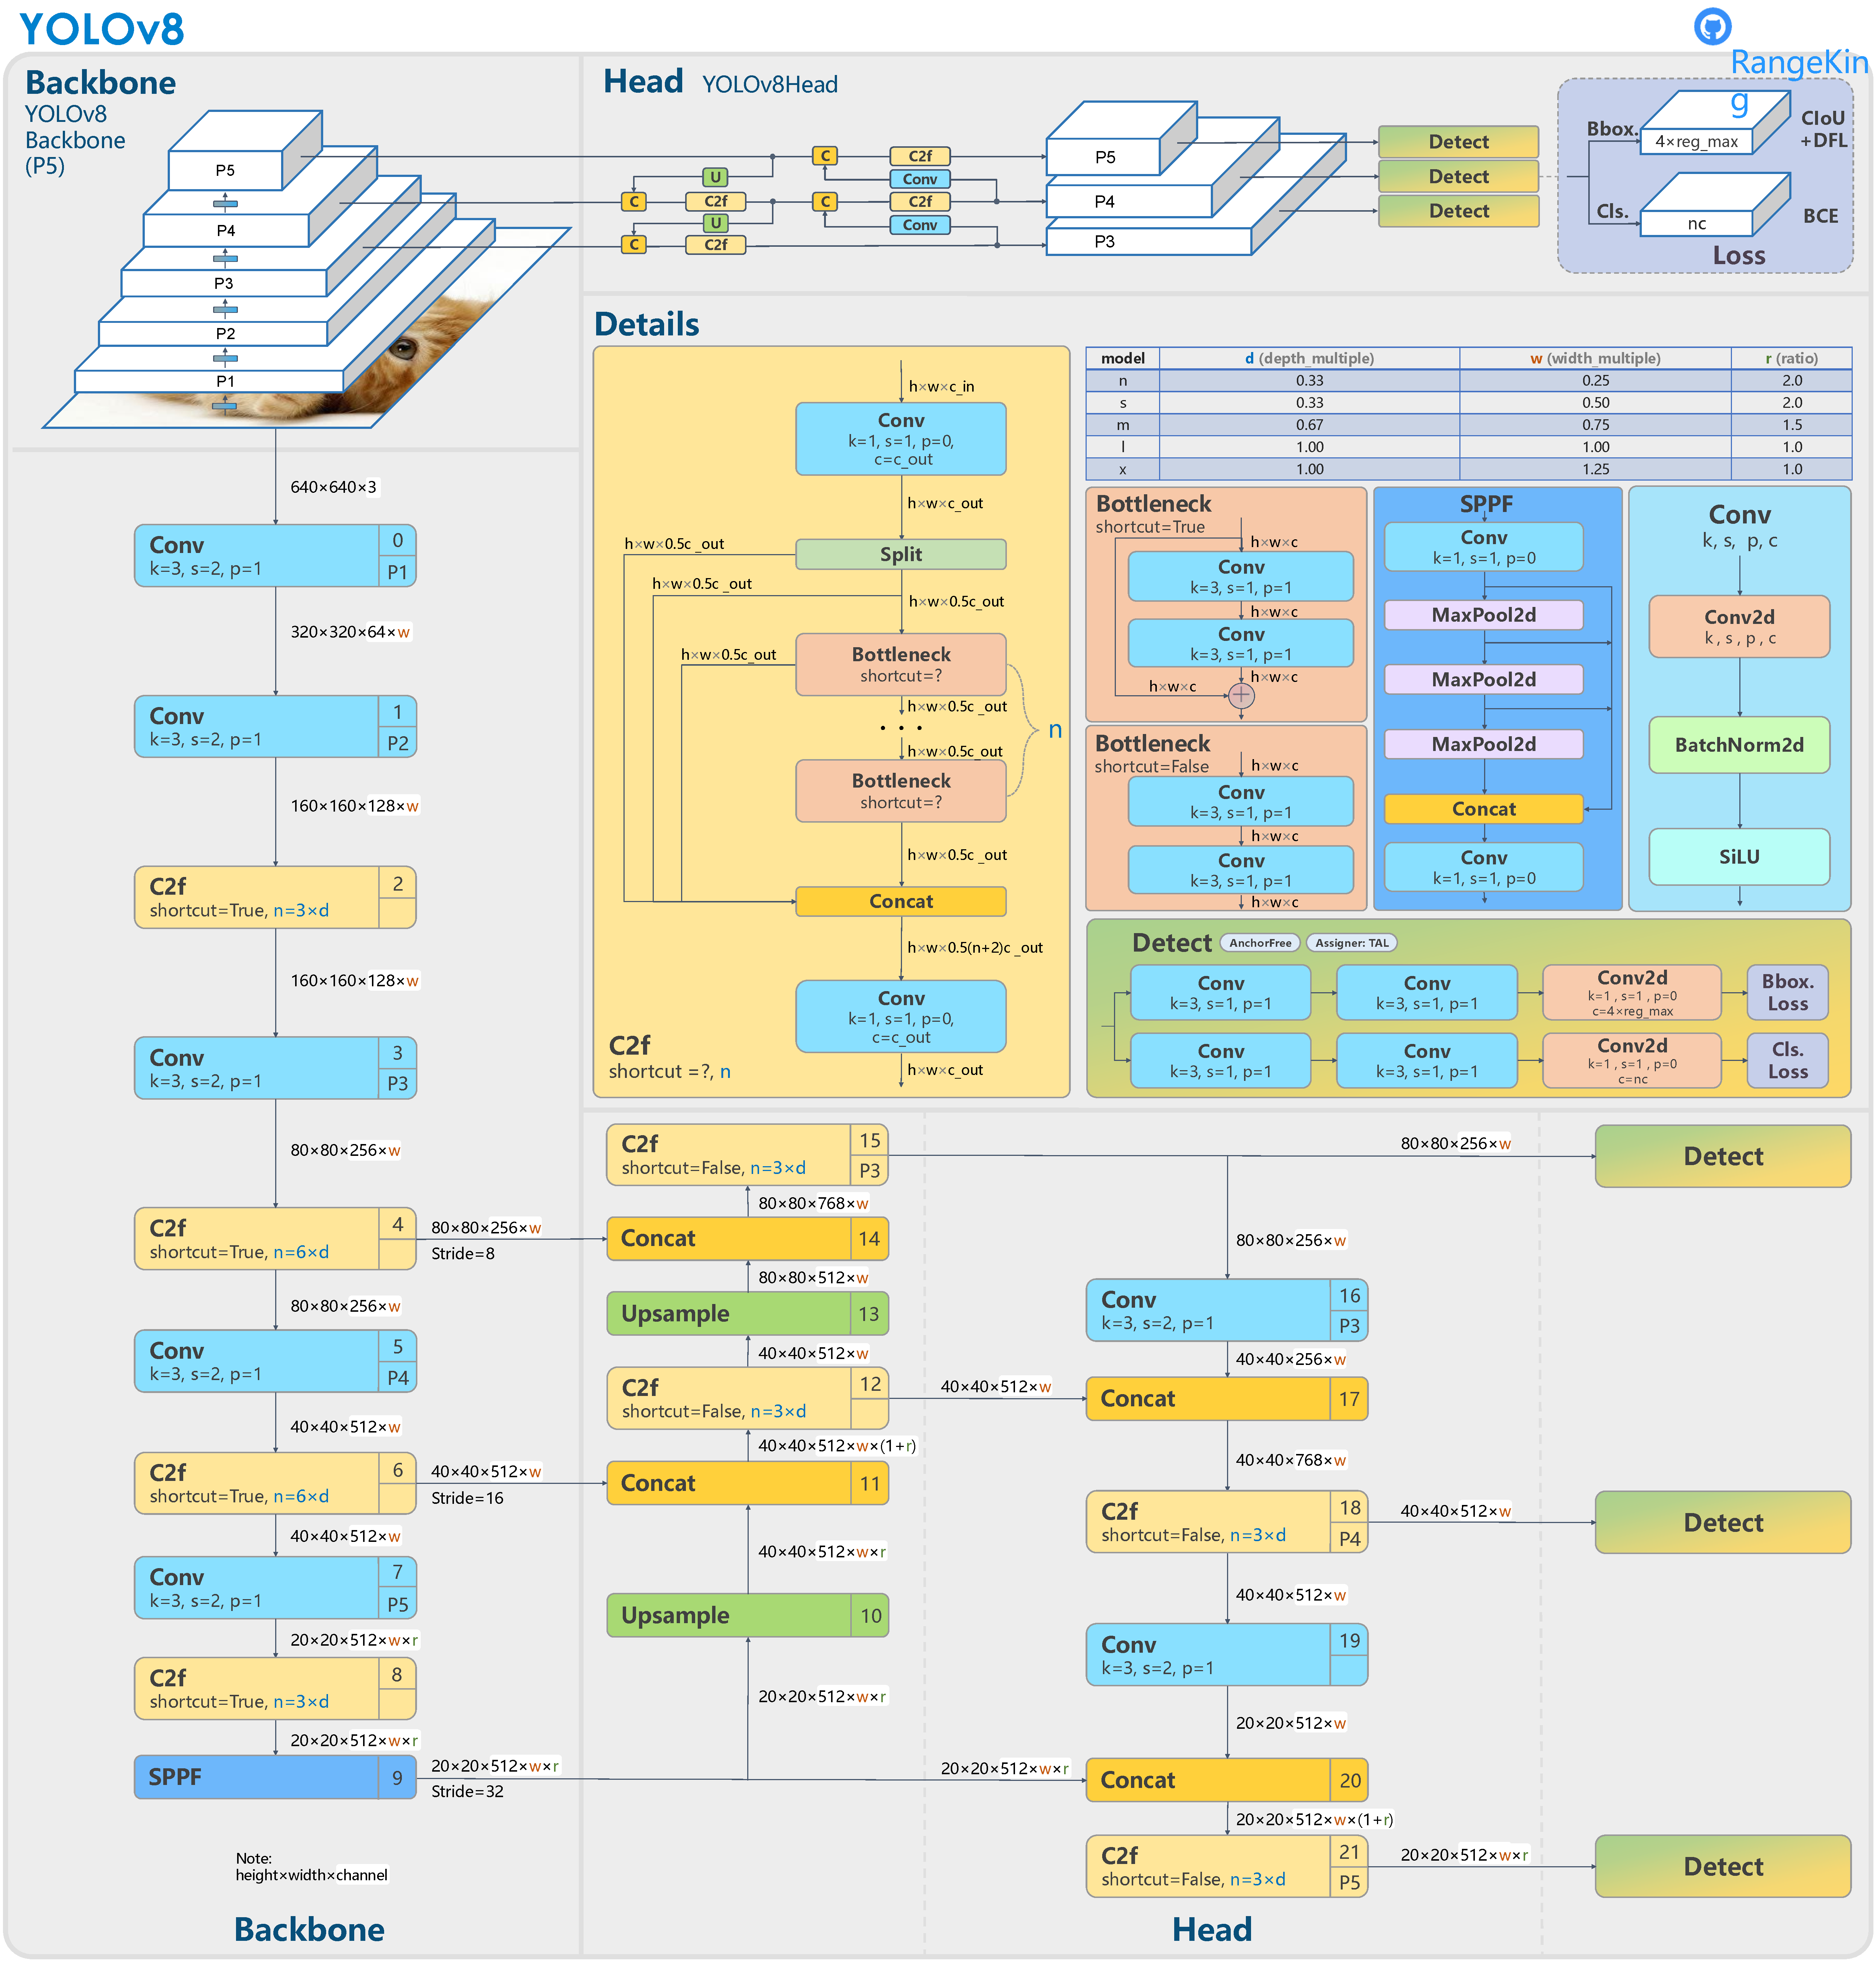
\includegraphics[width=0.8\linewidth]{pics/YOLOv8_structure.pdf}
    \caption{Overall YOLOv8 architecture and model scaling variables~\cite{yolov8_architecture_rangeking}}
    \label{fig:yolo_architecture_0}
\end{figure}

The backbone begins with strided convolutional layers that reduce spatial resolution while increasing channel
depth. These stages are interleaved with C2f blocks, which are described in the Ultralytics reference implementation
as a ``faster implementation of Cross-Stage Partial (CSP) bottleneck with 2 convolutions.'' The main purpose of these blocks is to improve
gradient flow and feature reuse while maintaining computational efficiency. At the deepest stage of the network,
YOLOv8 employs an SPPF (Spatial Pyramid Pooling -- Fast) module, which increases the effective receptive field
and improves multiscale context aggregation with relatively low computational overhead.

Overall, the main backbone components of YOLOv8 are:
\begin{itemize}
    \item convolutional blocks with Batch Normalization and SiLU activation,
    \item C2f feature extraction blocks,
    \item the SPPF module.
\end{itemize}

The C2f block itself is composed of several bottleneck units. Conceptually, such a block first reduces the number
of channels, then performs spatial feature transformation, and finally combines intermediate representations
to preserve useful information. This design improves feature propagation and reduces redundant computation while
retaining informative representations. Compared with earlier CSP-style blocks, C2f enables richer feature reuse
and more efficient gradient flow.

The neck follows a Path Aggregation Network (PAN)--FPN style design. In practice, this means that feature maps are upsampled, concatenated
with earlier backbone features, and then processed again using C2f blocks. This combination of top-down and bottom-up
feature fusion is central to YOLOv8's ability to detect objects across multiple scales. The reference YAML
architecture repeatedly uses Upsample, Concat, and C2f blocks before the final
Detect module. Such multiscale aggregation is particularly important for real-world datasets, where
object size can vary significantly across scenes.

The prediction head in YOLOv8 is both decoupled and anchor-free. Ultralytics describes YOLOv8 as using an anchor-free
split detection head, meaning that predictions are not tied to a predefined set of anchor box shapes. Instead,
the detector predicts bounding boxes and class scores directly from the feature maps. Compared with older anchor-based
YOLO variants, this simplifies the detection pipeline and removes the need for dataset-specific anchor tuning.

In an anchor-free detector, each spatial location on the feature map typically predicts:
\begin{itemize}
    \item whether an object is present,
    \item the class scores,
    \item the box coordinates or distances to the box boundaries.
\end{itemize}

The split head further separates the localization and classification tasks into distinct branches. This decoupling
allows the model to optimize these tasks more effectively, since object localization and semantic classification
impose different requirements on the learned feature representations.

Another important component of the YOLOv8 detection formulation is its use of distribution-based box regression.
The Ultralytics codebase includes a DFL module and the corresponding loss implementation, reflecting the use
of Distribution Focal Loss for bounding box parameterization. This improves localization precision by modeling
bounding box offsets as discrete probability distributions rather than relying solely on coarse direct regression.

\paragraph{Relevance of YOLOv8 for this thesis}

For a thesis focused on compiler-aware optimization of deep learning models for edge devices, YOLOv8, and especially
YOLOv8n, represents a highly suitable case study.

First, YOLOv8 offers a strong balance between detection accuracy and inference latency, which is one reason why
later detectors continue to use it as a baseline. Second, YOLOv8 has a mature deployment ecosystem. Ultralytics
supports export to a wide range of formats relevant for practical deployment, including ONNX, TensorRT, CoreML,
OpenVINO, and TFLite. This makes the model especially attractive for evaluating compiler and runtime behavior across
different hardware platforms.

In addition, YOLOv8 is not limited to object detection alone. The model family also supports segmentation,
classification, pose estimation, and oriented bounding box detection within the same software ecosystem.
This is particularly relevant in applied edge AI research, where systems often evolve from simple object
detection toward richer scene understanding tasks. As a result, YOLOv8 provides both architectural consistency
and practical flexibility.

For this thesis, YOLOv8n is of particular interest because it is small enough to run on many embedded platforms,
while still being architecturally complex enough to expose realistic deployment bottlenecks. The model includes
multiscale feature fusion, repeated tensor concatenations, SiLU activations, distribution-based box regression,
and post-processing stages. These properties make it a meaningful test case for studying compiler optimizations,
runtime scheduling, kernel efficiency, quantization behavior, and memory-system effects.

Despite being the smallest variant, YOLOv8n is not automatically optimal for every edge target. Several practical
challenges arise during deployment.

First, a low parameter count does not necessarily translate into low latency on all hardware platforms. YOLOv8n still
contains nontrivial tensor reshaping, concatenation, upsampling, and multiscale fusion operations. On desktop GPUs,
such operations may be efficiently hidden by optimized kernels and memory systems, whereas on edge CPUs and lightweight
accelerators the cost of memory movement can dominate the arithmetic workload. In such cases, the effective
execution becomes memory-bound rather than compute-bound.

Second, operator support and kernel efficiency vary significantly across deployment backends. Although YOLOv8 can
be exported to ONNX, TensorRT, TFLite, and other runtimes, the achieved performance depends strongly on how well
the target backend supports the specific operator set and graph structure of the model. In practice, operations
such as SiLU, concatenation-heavy neck structures, and certain post-processing steps may be implemented with
different levels of efficiency across frameworks. As a result, there is often a noticeable gap between the
theoretical Floating-Point Operation (FLOP) count of the model and the measured end-to-end latency.

Third, post-processing introduces an additional deployment challenge. Standard YOLOv8 detection still relies on
confidence filtering and non-maximum suppression after the forward pass. On GPU-based systems, this may require
transferring relatively large tensors from the device to the host, followed by post-processing on the CPU. Such
steps can add non-negligible latency and complicate the analysis of true end-to-end performance.

Overall, YOLOv8 is an interesting subject for deployment-oriented research because it combines architectural
complexity with competitive accuracy and speed.


\section{Challenges of edge deployment}

With the growing interest in on-device deployment, a clear gap has emerged between the training and inference
stages of machine learning models. While large models are typically trained in data centers using powerful GPUs,
inference is performed across a wide variety of environments subject to strict constraints on memory, latency,
and power consumption. These environments span heterogeneous hardware platforms - CPUs, GPUs, TPUs, NPUs,
and FPGAs - each differing in instruction sets, memory hierarchies, and supported data types. As a result,
model performance depends heavily on how well the deployment is adapted to the target hardware.

\noindent Deployment efficiency is characterized along four principal dimensions:
\begin{itemize}
\item \textbf{Latency} measures the time
required to process a single inference request and is the dominant constraint in real-time applications such
as object detection, where a response must be produced within a fixed time budget.
\item \textbf{Throughput}
captures the number of inference requests completed per unit of time and becomes the primary metric when
processing is batched or pipelined.
\item \textbf{Power consumption} reflects the energy cost of inference, which
is particularly critical on battery-powered or thermally constrained embedded devices.
\item \textbf{Memory
requirements} encompass both the storage needed for model weights and the working memory consumed by
intermediate activations during a forward pass, both of which can be hard limits on resource-constrained
hardware.
\end{itemize}

Machine learning models are typically developed in high-level Python frameworks such as TensorFlow or
PyTorch, which use dynamic execution: operations are dispatched immediately, control flow is resolved at
runtime, and tensors are created and destroyed on the fly. This flexibility comes at a cost. Every operation
passes through the Python interpreter; the Global Interpreter Lock (GIL)~\cite{python_capi_gil} limits parallel execution;
tensors and operators are heap-allocated Python objects; and each kernel dispatch requires the framework to resolve
device placement and memory management at runtime. Individually these overheads are small, but across a deep
network with thousands of operations they accumulate into a non-trivial fraction of end-to-end latency.

In deployment, models are therefore not run inside Python at all. Instead, they are executed by C++-based
runtimes, hardware-specific inference engines, or precompiled binaries targeting accelerators such as GPUs,
NPUs, and FPGAs~\cite{chen2018tvm,onnxruntime_execution_providers,nvidia_tensorrt_docs}. These runtimes execute
pre-compiled computation graphs, call highly optimized kernels
directly, and avoid Python entirely. However, simply exporting a model out of Python does not automatically
guarantee speedups. To fully benefit, the model must first be compiled into a static or semi-static graph,
then optimized through operator fusion, memory planning, quantization, and layout transformations, and
finally adapted to the instruction set and memory hierarchy of the target hardware. Without this compilation
step, a deployed runtime may still execute inefficient kernels or suboptimal data flows.

A further challenge is that highly optimized kernel libraries such as cuDNN and oneDNN are not
automatically optimal for all deployment regimes. Although these libraries support both training and
inference, many of their fastest implementations rely on sufficient arithmetic intensity, data reuse,
vectorization, and parallel work to amortize scheduling and dispatch overheads. These conditions are
often easier to satisfy in training or high-throughput inference, where larger batches allow weights and
activation tiles to be reused across multiple samples.

In real-time edge inference, however, batch size is often fixed to one in order to minimize response
latency. Under this regime, the computation may expose less parallelism and less reuse per invocation.
On GPUs, this can reduce occupancy and make CUDA kernel-launch overhead, memory traffic, and
operator fragmentation more visible in the end-to-end latency. On CPUs, the analogous issue is not GPU
occupancy but reduced Single Instruction, Multiple Data (SIMD) utilization, less effective cache blocking, thread-management overhead,
and layout-conversion overheads. As a result, batch-size-one inference can be limited not only by peak
compute throughput, but also by memory movement, runtime overhead, and the ability of the compiler or
runtime to fuse operators and select kernels specialized for small-batch execution.

Graph-level compilers address this by operating on the entire computation graph rather than dispatching one
operator at a time. With global visibility over operators, data dependencies, and tensor lifetimes,
a compiler can fuse multiple operations into a single kernel, fold constants, eliminate dead branches, and
reorder associative operations to improve locality. It can also select a single data layout (channels-first NCHW, channels-last NHWC, or
a blocked format) that suits the target hardware and insert only the minimal number of layout conversions,
avoiding the unnecessary transposes that arise when operators from different libraries are composed naively.


\section{ML compilers and inference runtimes}

Deep learning compilers specialize traditional compiler ideas for tensor programs and neural-network graphs
~\cite{li2020deep, zhang2023compiler, thangamani2024survey, zhang2026new}.
They address the gap between high-level model definitions and heterogeneous deployment targets
by lowering neural-network graphs through one or more intermediate representations, applying graph-level and
operator-level optimizations, and generating target-specific code or calls to optimized backend libraries.
So the code, expressed in a framework such as PyTorch, TensorFlow, JAX, or
as an ONNX graph is transformed into an executable form suitable for a particular target, such as a CPU,
GPU, NPU, FPGA, or dedicated accelerator.

Most ML compiler stacks follow a layered structure, illustrated in Figure~\ref{fig:compflow}.
The frontend first captures or imports the model from a source framework such as
PyTorch~\cite{paszke2019pytorch}, TensorFlow~\cite{abadi2016tensorflow}, or
JAX~\cite{frostig2019compiling}. In practical deployment pipelines, this import step is often
mediated by an exchange format such as ONNX~\cite{microsoft2017onnx}. Other representations are
more closely tied to particular compiler ecosystems: TorchScript was historically used for PyTorch
graph capture and deployment, FX graphs are used in the PyTorch 2.x compilation pipeline
~\cite{reed2022torch}, High-Level Optimizer (HLO) is the central Intermediate Representation (IR) in Accelerated Linear Algebra (XLA)~\cite{openxla_hlo_to_thunks_docs}, and
StableHLO provides a more portable HLO-based representation in the OpenXLA/Multi-Level Intermediate Representation (MLIR) ecosystem
~\cite{openxla_stablehlo_docs}.

The imported program is then converted into the compiler's internal intermediate representation.
The graph optimization stage then applies framework-agnostic transformations: operator fusion
and simplification, constant folding, dead-branch
elimination, and memory planning. The resulting high-level IR is subsequently lowered to a
loop-level representation where tiling, vectorization, and memory-access scheduling are applied for the
specific target. Finally, the code generation backend performs instruction selection, register
allocation, and emits target-specific machine code.

Once compiled, the model is managed by an ML runtime, which handles execution orchestration
(loading the compiled artifact and scheduling its execution), memory allocation for intermediate tensors,
hardware interfacing, and integration with vendor libraries.

Modern systems differ mainly in where they place the boundary between compilation, runtime
dispatch, and vendor-specific libraries. For example, TensorFlow XLA lowers TensorFlow or JAX-style
computations through HLO-based representations and uses XLA backends to generate efficient
target-specific execution~\cite{tensorflow_xla_architecture,xla_hlo_tooling}. PyTorch 2.x follows a
different route: TorchDynamo captures Python-level execution into FX graphs, AOTAutograd handles
ahead-of-time graph extraction for training-related graphs, and TorchInductor lowers the resulting
graphs to optimized CPU or GPU code~\cite{pytorch_torch_compile,pytorch_compile_faq,pytorch_2x}.
Apache TVM exposes a more explicit compiler stack for heterogeneous deployment, combining
graph-level optimization with tensor-level scheduling and auto-tuning for CPUs, GPUs, and
edge-oriented targets~\cite{apache_tvm_home, chen2018tvm}. MLIR-based systems, including IREE
and TensorFlow MLIR, use multiple IR dialects to represent computation at different abstraction
levels and to support flexible lowering pipelines for heterogeneous systems
~\cite{lattner2021mlir,mlir_overview,tensorflow_mlir_overview,iree_home}. ONNX Runtime, in
contrast, is primarily an inference runtime built around the ONNX format; it performs graph
optimizations and delegates execution to hardware-specific execution providers such as CPU, CUDA,
TensorRT, OpenVINO, CoreML, or other backends~\cite{onnxruntime_home,onnxruntime_execution_providers}.

These systems therefore solve overlapping but not identical problems. TVM and XLA are closer to
full compiler stacks with explicit IR lowering and code generation, TensorRT is a vendor-specific
inference compiler and runtime for NVIDIA GPUs, PyTorch 2.x integrates compilation into an eager
framework workflow, MLIR-based systems provide reusable infrastructure for building compiler
pipelines, and ONNX Runtime emphasizes portable model execution through execution providers.
For edge-AI deployment, this distinction is important because performance depends not only on the
model architecture, but also on the chosen representation, compiler lowering path, operator coverage,
precision support, runtime overhead, and the quality of the target-specific backend.

Overall, the architecture of a deep-learning compiler can be viewed as a pipeline composed of a
frontend, one or more intermediate representations, and a backend. The IR connects these stages and often appears
at multiple levels of abstraction, ranging from high-level graph IR to low-level operator or tensor IR.

\paragraph{The high-level IR (Graph IR)} represents the computation graph of a deep-learning model
at a level above hardware-specific code generation. It captures operators, tensors, data dependencies,
and in some systems also control flow, while remaining mostly hardware-independent. Its purpose is
to provide a representation on which the compiler frontend can perform graph-level optimizations
before lowering the model to a lower-level IR for scheduling, code generation, and hardware-specific
optimization~\cite{li2020deep}.

A common representation is a directed acyclic graph (DAG)(see listing~\ref{lst:dag_graph_ir}), where nodes correspond
to neural-network
operators such as convolution, pooling, reshape, or activation functions, and edges correspond to tensors
flowing between operators. This representation allows the compiler to analyze dependencies between
operators and apply optimizations. However, pure DAG-based representations
can be limited when the computation scope or control flow must be represented explicitly. For this reason,
some compiler IRs also use let-binding (see listing~\ref{lst:let_binding_ir}), which represents each intermediate
tensor as a named binding,
or functional representations (see listing~\ref{lst:function_based_ir}), which views computation
as a collection of functions, where each function contains
operations/instructions and has explicit inputs and outputs. For example, TVM Relay combines
DAG-style graph representation with let-binding ideas, while XLA HLO uses a function-based representation
organized around modules, computations, and instructions~\cite{li2020deep}.

The high-level IR must also encode tensor-specific information that is essential for deep-learning
optimization. This includes tensor shapes, possibly dynamic dimensions, data layouts such as NCHW or
NHWC, broadcasting rules, reduction operations, and support for custom operators. This information is
needed to infer valid transformations, select efficient layouts, and preserve correctness when the graph is
later lowered to backend-specific code. Thus, the high-level IR acts as the bridge between framework-level
model definitions and lower-level compiler stages: it is expressive enough to describe deep-learning
models, but abstract enough to enable hardware-independent graph optimization.

\begin{listing}[htbp]
\begin{minted}[fontsize=\small, breaklines=true]{text}
DAG-based graph IR:

x ----\
       conv2d ----> z ----> relu ----> a ----\
w ----/                                      add ----> y
bias ---------------------------------------/

Nodes:
  conv2d, relu, add

Edges:
  x, w, z, a, bias, y
\end{minted}
\caption{Example of a DAG-based graph IR representation.}
\label{lst:dag_graph_ir}
\end{listing}

\begin{listing}[htbp]
\begin{minted}[fontsize=\small, breaklines=true]{text}
Let-binding-based IR:

let z = conv2d(x, w) in
let a = relu(z) in
let y = add(a, bias) in
return y
\end{minted}
\caption{Example of a let-binding-based IR representation.}
\label{lst:let_binding_ir}
\end{listing}

\begin{listing}[htbp]
\begin{minted}[fontsize=\small, breaklines=true]{text}
Function-based IR:

function forward(x, w, bias):
    z = conv2d(x, w)
    a = relu(z)
    y = add(a, bias)
    return y
\end{minted}
\caption{Example of a function-based IR representation.}
\label{lst:function_based_ir}
\end{listing}


\paragraph{The low-level IR}
The low-level IR represents the computation of a deep-learning model in a more fine-grained form
than the high-level graph IR. While the high-level IR is mainly used to describe operators, tensors,
and graph-level dependencies, the low-level IR is closer to the actual implementation of each
operator or fused subgraph. It exposes loop structure, memory accesses, tensor indexing,
scheduling decisions, and target-specific information, making it the main interface for
hardware-dependent optimizations and code generation~\cite{li2020deep}.

A common design in low-level IRs is to separate the description of what is computed from
how it is computed. Halide-inspired IRs, used for example in TVM, follow this idea by
separating the tensor computation from its schedule. The computation defines the mathematical
operation, while the schedule controls implementation choices such as tiling, loop reordering,
vectorization, parallelization, memory placement, and unrolling. This separation is useful because
the same operator can be mapped differently depending on the target hardware, such as an Advanced RISC Machine (ARM)
CPU, an NVIDIA GPU, or a specialized accelerator.

Another important family is polyhedral-based IRs. These represent loop nests and memory
accesses using mathematical sets, affine transformations, and dependence relations. Such
representations are well suited for optimizing regular tensor computations, because they make it
possible to reason about loop transformations such as fusion, tiling, skewing, mapping, and
parallelization. However, polyhedral approaches are most effective when loop bounds and memory
accesses can be described statically and regularly, which can limit their applicability for highly
dynamic or irregular model structures.

Some compiler systems use their own low-level IRs instead of directly adopting Halide- or
polyhedral-style representations. For example, Glow~\cite{rotem2018glow} uses an instruction-based low-level IR over
explicit memory regions, while MLIR~\cite{mlir_overview} provides a multi-level compiler infrastructure based on
dialects, allowing tensor, linear algebra, affine, Low-Level Virtual Machine (LLVM)~\cite{lattner2004llvm}, and hardware-specific
abstractions to coexist in the same framework.
XLA HLO can also serve both high-level and lower-level roles, since it is
fine-grained enough to express many target-specific optimization decisions while still preserving
tensor-level semantics.

The low-level IR is eventually lowered to executable code or runtime calls, often through mature
compiler infrastructures such as LLVM, CUDA, OpenCL, or vendor-specific code generators. This
stage may be performed just-in-time (JIT), where code is generated at runtime using available
shape and hardware information, or ahead-of-time (AOT), where executable binaries are generated
before deployment. In edge-AI deployment, the low-level IR is especially important because
performance depends strongly on hardware-specific choices such as memory hierarchy usage,
vector width, cache behavior, tensor layout, and available accelerator instructions.

\paragraph{Frontend Optimizations}
It is easier to identify optimization opportunities when the machine learning model is represented
as a complete computation graph rather than as isolated operators. Frontend optimizations are
therefore applied at the graph or high-level IR level, before the model is lowered to hardware-specific
backend code. These transformations are mostly hardware-independent: they simplify the graph,
remove redundant operations, expose fusion opportunities, and reduce memory traffic, but they do
not yet define how each operation is implemented on a particular CPU, GPU, or accelerator.

Li et al.~\cite{li2020deep} classify frontend optimizations in deep-learning compilers into three
main categories: node-level, block-level, and dataflow-level optimizations.

\begin{itemize}
    \item \textbf{Node-level optimizations} operate on individual graph nodes. They include
    node elimination and node replacement, where unnecessary or expensive nodes are removed
    or replaced by cheaper equivalent operations. Examples include removing identity operations,
    eliminating padding nodes with zero padding width, or replacing a redundant reshape with
    direct tensor forwarding.

    \item \textbf{Block-level optimizations} operate on small local subgraphs. They include
    algebraic simplification, strength reduction, constant folding, operator fusion, and operator
    sinking. For example, a sequence such as convolution, bias addition, and activation can be
    fused into a single higher-level operation, reducing intermediate tensors and kernel-launch
    overhead.

    \item \textbf{Dataflow-level optimizations} operate globally across the computation graph.
    They include common sub-expression elimination, dead code elimination, static memory
    planning, and layout transformation. These optimizations exploit the global graph structure
    to avoid recomputation, remove unused branches, reuse memory buffers, and select tensor
    layouts that are more suitable for later backend execution.
\end{itemize}

Figure~\ref{fig:frontend_optimization_examples} illustrates representative examples of these
frontend graph transformations.

\begin{figure}[h]
    \centering
    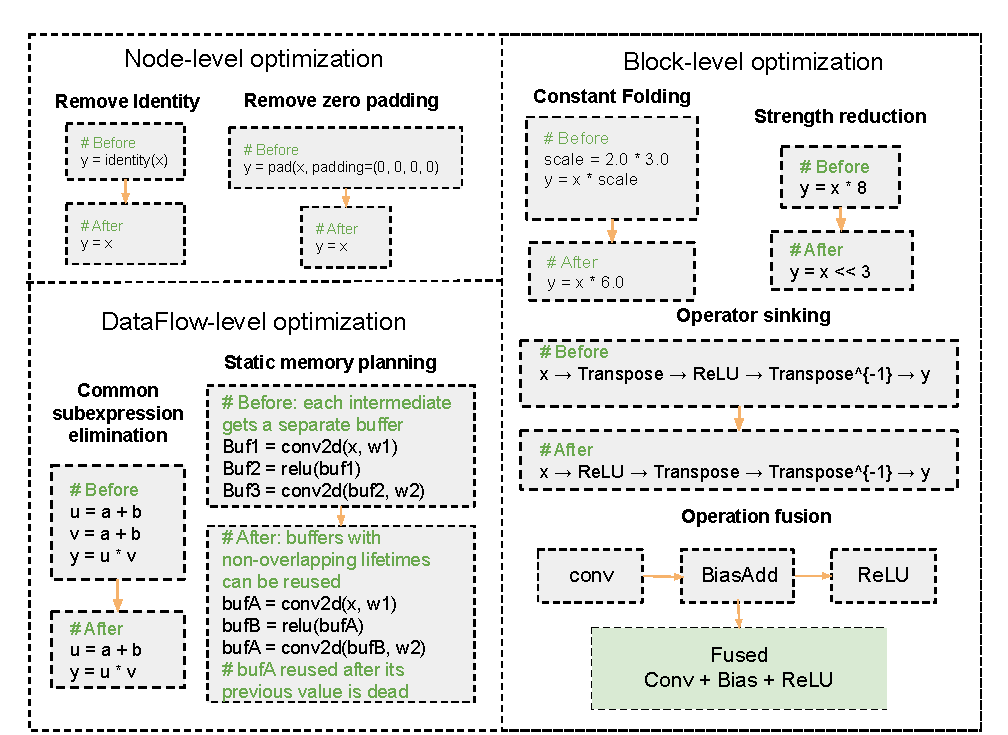
\includegraphics[width=\textwidth]{pics/frontend_optimization_examples.pdf}
    \caption{Representative examples of frontend graph optimizations in deep-learning compilers.
    Node-level optimizations remove or replace individual redundant nodes, block-level optimizations
    simplify or fuse local subgraphs, and dataflow-level optimizations exploit the global computation
    graph to remove redundant computation or reuse memory buffers.}
    \label{fig:frontend_optimization_examples}
\end{figure}

\paragraph{Backend Optimizations}

Backend optimizations form the target-specific part of a deep-learning compiler. After the model
has been represented in a graph or tensor-level IR, the backend lowers this representation to
executable code, optimized kernels, or calls into vendor libraries. In practice, high performance is
often achieved by combining library-based execution, such as cuDNN, MIOpen, oneDNN, or BLAS
kernels, with compiler-generated transformations that specialize the computation for the target
architecture. These transformations include mapping low-level IR patterns to hardware intrinsics
or optimized micro-kernels, assigning intermediate tensors to appropriate memory scopes, improving
data locality through cooperative fetching and explicit memory allocation, hiding memory latency
through scheduling and hardware thread switching, and applying loop transformations such as
fusion, tiling, reordering, unrolling, and sliding-window optimizations. The backend also exposes
parallelism at multiple granularities, including SIMD vectorization, CPU multi-threading, GPU
thread/block parallelism, and accelerator-specific execution units.
Figure~\ref{fig:hardware_specific_optimizations_dl_compilers}
summarizes several representative backend-level optimization techniques used in deep-learning
compilers.

\begin{figure}[h]
    \centering
    \includegraphics[width=\textwidth]{pics/overview_of_hardware_spec_optimizations_applied.pdf}
    \caption{Overview of hardware-specific optimizations applied in deep-learning compilers.
    Reproduced from Li et al.~\cite{li2020deep}.}
    \label{fig:hardware_specific_optimizations_dl_compilers}
\end{figure}


A central difficulty is that these optimizations create a large, hardware-dependent search space.
Even for a single convolution or matrix multiplication, the compiler may need to choose tile sizes,
loop orders, memory layouts, vector widths, thread/block mappings, unrolling factors, and intrinsic
implementations. The best configuration depends on the target architecture, cache hierarchy,
memory bandwidth, register pressure, available parallelism, and supported instruction set. As a
result, many deep-learning compilers incorporate auto-tuning mechanisms. Auto-tuning defines a
space of valid schedules and searches for high-performing implementations using empirical
measurements, analytical or learned cost models, and heuristic search methods such as genetic
algorithm (GA)~\cite{Goldberg1989}, reinforcement learning (RL)~\cite{mnih2015human_level_control},
simulated annealing (SA)~\cite{bertsimas1993simulated}, or evolutionary search~\cite{ashouri2018survey}.

Although many standard deep-learning kernels are highly optimized, model development often progresses faster than
backend kernel support. New architectures can introduce operators or computation patterns that are not yet available
as optimized library kernels or compiler-generated implementations. In such cases, the computation may fall back to
unfused operator sequences or generic implementations, causing additional kernel launches, intermediate memory traffic,
reduced locality, and significant runtime overhead.

%\section{Hailo Compiler}

\begin{figure}[h]
    \centering
    \includegraphics[width=1.0\linewidth]{pics/compiler_structure_custom.pdf}
    \caption{Flow of an ML model from definition through compilation and runtime execution on hardware.}
    \label{fig:compflow}
\end{figure}


\subsection{Apache TVM}

Apache TVM~\cite{chen2018tvm} is an open-source machine learning compiler stack that treats model deployment as a
compiler problem.
Rather than dispatching operators to a fixed set of vendor-provided kernels, TVM imports a model, applies graph-level
transformations (constant folding, operator fusion, layout rewriting), lowers individual operators into explicit
loop-based tensor programs, and then searches for hardware-efficient implementations through automated schedule
tuning.
This pipeline follows the general compiler flow described in the previous section, but exposes each stage to the
user, making TVM useful both as a deployment tool and as a research platform for studying how compilation choices
affect inference performance.

The central design principle is the separation between computation and schedule.
The computation defines what is computed; the schedule defines how it maps to hardware.
For the same convolution, the compiler can explore different tile sizes, loop orders, vector widths, memory staging
strategies, and thread/block mappings for the target.
In practice, TVM automates this via MetaSchedule: candidate schedules are generated, benchmarked on the device,
and ranked by measured latency, producing a hardware-specific binary without manual kernel engineering.

TVM's main strength is hardware portability and the ability to unlock optimisation paths not available in
fixed-kernel runtimes.
On ARM CPUs, schedule search can target NEON vector intrinsics explicitly; on NVIDIA GPUs, FP16 MetaSchedule tuning
enables WMMA tensorisation for convolutional operators.
Its limitations are a complex compilation workflow and performance that depends heavily on the quality and duration
of the tuning campaign: an untuned TVM build may not outperform generic runtimes.
In this thesis, TVM is evaluated with MetaSchedule on both the Jetson Orin Nano GPU and the Raspberry Pi~5 CPU,
serving as a reference for what an open, tunable compiler achieves relative to TensorRT and ONNX Runtime.

\paragraph{Tensor expression and scheduling: a concrete example.}
The computation--schedule separation is most clearly illustrated with matrix multiplication.
The mathematical operation is:
\begin{equation}
C[i,j] = \sum_k A[i,k] \cdot B[k,j]
\end{equation}
In TVM's tensor expression API this is written as a pure computation definition, with no implementation
detail:
\begin{minted}[fontsize=\small, breaklines=true]{python}
from tvm import te
M, N, K = 1024, 1024, 1024
A = te.placeholder((M, K), name="A")
B = te.placeholder((K, N), name="B")
k = te.reduce_axis((0, K), name="k")
C = te.compute(
    (M, N),
    lambda i, j: te.sum(A[i, k] * B[k, j], axis=k),
    name="C"
)
\end{minted}
This definition describes the mathematical computation only.
It does not yet specify loop ordering, blocking, vectorisation, or parallel execution.

\paragraph{Scheduling and kernel mapping.}
To obtain an efficient implementation, TVM applies scheduling decisions that determine how the tensor
computation maps to loops, threads, and memory.
Typical transformations include tiling, loop reordering, vectorisation, unrolling, and thread binding.
For a CPU target these translate to cache-friendly blocking, parallelisation across cores, and SIMD
vectorisation of the innermost loop:
\begin{minted}[fontsize=\small, breaklines=true]{python}
s = te.create_schedule(C.op)
i, j = C.op.axis
k = C.op.reduce_axis[0]
io, ii = s[C].split(i, factor=32)
jo, ji = s[C].split(j, factor=32)
s[C].reorder(io, jo, k, ii, ji)
s[C].parallel(io)
s[C].vectorize(ji)
\end{minted}
For a GPU target, the same computation is instead mapped to CUDA thread blocks and warps:
\begin{minted}[fontsize=\small, breaklines=true]{python}
bx, tx = s[C].split(i, factor=16)
by, ty = s[C].split(j, factor=16)
s[C].bind(bx, te.thread_axis("blockIdx.x"))
s[C].bind(by, te.thread_axis("blockIdx.y"))
s[C].bind(tx, te.thread_axis("threadIdx.x"))
s[C].bind(ty, te.thread_axis("threadIdx.y"))
\end{minted}
In both cases the computation definition is unchanged; only the schedule differs.
MetaSchedule automates exactly this search: it generates candidate schedules, measures their latency
on the target device, and selects the best-performing one, producing a hardware-specific binary without
manual kernel engineering.


\subsection{TensorRT}

TensorRT~\cite{nvidia_tensorrt_docs} is NVIDIA's inference compiler and runtime for NVIDIA GPUs.
Unlike TVM, it is not hardware-portable: it specializes a model for a concrete target platform, GPU architecture,
precision regime, and software stack, and produces a serialized engine encoding a fixed execution strategy.
A model is imported via ONNX; the builder then applies graph-level rewrites (constant folding, layer fusion,
dead-layer elimination), propagates shape and precision constraints, and empirically benchmarks multiple
implementation candidates (called tactics) for each layer or fused subgraph.
The best-performing tactic on the target device is embedded into the final engine.
This ahead-of-time empirical optimization is the central reason for TensorRT's strong practical
performance~\cite{nvidia_tensorrt_perf}.

Effective performance depends on Tensor Cores being utilizable.
For large convolutions and matrix multiplications, TensorRT selects implementations backed by cuDNN or cuBLASLt
that use Tensor Core instructions when shapes, data layouts, and precision satisfy the hardware constraints.
Operators not supported by TensorRT must be rewritten, decomposed, or replaced through the plugin interface.
The \path{IPluginV3} interface allows a hand-written CUDA or CUTLASS kernel to replace a subgraph while keeping
all surrounding layers in the standard TensorRT pipeline.
In the typical workflow, the target subgraph is replaced in the ONNX export using ONNX GraphSurgeon, and TensorRT
embeds the plugin as a first-class component during engine building.
This mechanism enables targeted replacement of persistent bottlenecks without abandoning TensorRT's graph-level
optimizations for the rest of the model.

Compared with TVM, TensorRT is narrower but more mature: it prioritises deployment effectiveness on NVIDIA hardware
over portability or research transparency.
Compared with ONNX Runtime, it is more aggressive on supported NVIDIA targets, performing deep kernel selection
and tactic benchmarking, rather than routing execution through interchangeable execution providers.
Its main limitations are GPU vendor lock-in, limited introspection of tactic selection, and performance degradation
at boundaries with unsupported operators where reformatting or data-type conversions break the fusion chain.
In this thesis, TensorRT serves two roles: it is the strongest latency baseline on the Jetson Orin Nano GPU, and
its plugin interface is used to study the overhead boundary of the standard engine by replacing the C2f subgraph
with a custom kernel (Section~\ref{sec:plugin}).



\cleardoublepage
\section{Quantization and Mixed Precision}

Quantization is one of the main techniques used to reduce the cost of neural-network inference on
resource-constrained hardware. A trained neural network is usually represented using floating-point
parameters and activations. Let's assume that a network has $L$ layers with learnable parameters
$\{W_1, W_2, \ldots, W_L\}$, and let $\theta$ denote the collection of all trainable parameters.
For a supervised learning problem, the model is trained by minimizing the empirical risk

\begin{equation}
\mathcal{L}(\theta) = \frac{1}{N} \sum_{i=1}^{N} l(x_i, y_i; \theta),
\end{equation}

where $(x_i, y_i)$ denotes an input sample and its corresponding label, $l(x_i, y_i; \theta)$ is
the loss function, and $N$ is the number of training samples. After training, the parameters
$\theta$ are typically stored in floating-point precision, and inference also produces intermediate
activation tensors between layers.

The goal of quantization is to represent these floating-point weights and activations using
lower-precision numerical formats, most commonly 8-bit integers. This can reduce model size,
memory bandwidth requirements, cache pressure, and arithmetic cost, which is especially important
for edge devices and accelerators with limited memory and power budgets. In practical terms,
quantization defines a mapping from a real-valued tensor to a discrete set of representable values.
If this mapping is chosen carefully, the model can run with substantially lower computational and
memory cost while preserving most of its original accuracy.

Surveys by Gholami et al.~\cite{gholami2022survey} and Rokh et al.~\cite{rokh2023comprehensive}
provide broad taxonomies of quantization methods, including post-training quantization,
quantization-aware training, uniform and non-uniform quantization, and mixed-precision
approaches. Practical integer-only inference is commonly associated with the work of
Jacob et al.~\cite{jacob2018quantization}, which describes how neural networks can be executed
using integer arithmetic during inference. Later post-training methods, such as
AdaRound~\cite{nagel2020up}, further improve quantized model accuracy by optimizing the
rounding decisions used when mapping floating-point weights to low-precision values.

Gholami et al.~\cite{gholami2022survey} defines a function that can quantize NN weight and activations to a finite
set of values:

\begin{equation}
Q(r) = \operatorname{Int}(r / S) - Z,
\end{equation}

where $Q$ is the quantization operator, $r$ is a real valued input (activation or weight), $S$ is a real valued scaling
factor, and $Z$ is an integer zero point. So the function $Q(r)$ is mapping a real value to an integer value through a
rounding operation. This method is a uniform quantization, as quantization levels are uniformely spaced.

Real values  $r$ can be recovered form the the quantized values $Q(r)$ through an operation that is referred to as
dequantization:

\begin{equation}
\tilde{r} = S \bigl(Q(r) + Z\bigr)
\end{equation}

Because the operator $\operatorname{Int}(\cdot)$ involves rounding, the dequantized value
$\tilde{r}$ is generally only an approximation of the original floating-point value $r$. The difference
between them is the quantization error. For uniform quantization, the quantization levels are
equally spaced, so the error is controlled mainly by the scale $S$, the zero point $Z$, and the
range of values that is mapped into the available integer domain. A smaller scale gives finer
resolution, but only over a smaller real-valued range; a larger scale covers a wider range, but
with coarser quantization steps. Thus, quantization introduces a trade-off between clipping error
and rounding error.

A central design choice is the clipping range $[\alpha, \beta]$, which defines the range of real
values represented by the quantizer. For a $b$-bit integer representation, a common scale choice is

\begin{equation}
S = \frac{\beta - \alpha}{2^b - 1},
\end{equation}

where $\alpha$ and $\beta$ are the lower and upper clipping bounds. Values outside this interval
are clipped before quantization, while values inside the interval are rounded to the nearest
available quantization level. Choosing the clipping range is often called calibration. A
simple calibration method uses the minimum and maximum observed values, but this can be
sensitive to outliers: a few extreme activation values may enlarge the range and reduce the
effective resolution for the majority of values. Alternative calibration methods therefore use
percentiles, mean-squared-error minimization, or divergence-based criteria to choose a range that
better preserves the distribution of the tensor~\cite{gholami2022survey}.

\paragraph{Symmetric and asymmetric quantization}
Uniform quantization can be either symmetric or asymmetric. In symmetric quantization, the
clipping range is centered around zero, so $\alpha = -\beta$. This usually allows the zero point to
be removed:

\begin{equation}
Q(r) = \operatorname{Int}\left(\frac{r}{S}\right).
\end{equation}

This form is attractive because it simplifies the arithmetic and is especially common for weight
quantization. For example, matrix multiplication and convolution can be implemented more
efficiently when the zero point is zero, since fewer correction terms are needed during integer
accumulation. However, symmetric quantization may waste representational levels when the tensor
distribution is strongly skewed. This often happens for activations after ReLU, where the values
are non-negative. In such cases, asymmetric quantization can use the available integer range more
efficiently by allowing a non-zero zero point $Z$ and a clipping interval that is not centered around
zero. Figure~\ref{fig:symmetric_asymmetric_quantization} illustrates the difference between symmetric
and asymmetric quantization.

\begin{figure}[htbp]
    \centering
    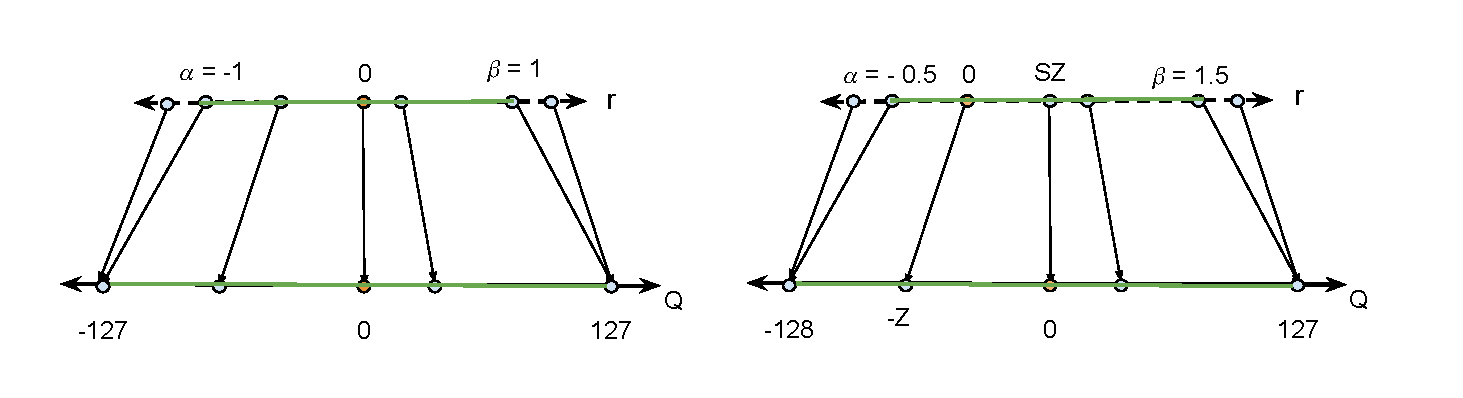
\includegraphics[width=1.1\textwidth]{pics/sym_nonsym_quantization.pdf}
    \caption{Illustration of symmetric and asymmetric quantization. In symmetric quantization,
    the real-valued clipping range is centered around zero, so the zero point can be set to
    $Z=0$. In asymmetric quantization, the clipping range is shifted to better match an
    imbalanced tensor distribution, such as non-negative activations after ReLU. Adapted from
    Gholami et al.~\cite{gholami2022survey}.}
    \label{fig:symmetric_asymmetric_quantization}
\end{figure}

For symmetric quantization, there are also different conventions for mapping the real-valued
range into the integer range. A full-range INT8 scheme uses the interval $[-128,127]$, while a
restricted-range scheme uses $[-127,127]$. The corresponding scale can be written as

\begin{equation}
S_{\mathrm{full}} = \frac{2\max(|r|)}{2^n - 1},
\end{equation}

or, for the restricted symmetric range,

\begin{equation}
S_{\mathrm{restricted}} = \frac{\max(|r|)}{2^{n-1} - 1}.
\end{equation}

The full-range scheme uses one additional representable value, while the restricted scheme keeps
the positive and negative ranges balanced. In practice, the best convention depends on the
hardware backend, the runtime format, and the kernels used by the inference engine.

\paragraph{Static and dynamic quantization}
Another important distinction is when the quantization parameters are determined. For weights,
the range can usually be computed statically, because trained parameters are fixed during
inference. Activations are more difficult because their distributions depend on the input sample.
In dynamic quantization, activation ranges are computed at runtime for each input or batch.
This can improve accuracy because each tensor is quantized using its actual observed range, but
it adds overhead from computing statistics such as minimum and maximum values during
inference. In static quantization, activation ranges are estimated before deployment using a
small calibration dataset and then kept fixed during inference. This avoids runtime calibration
overhead and is therefore more attractive for low-latency deployment, but it can reduce accuracy
if the calibration set does not represent the true deployment distribution well. Gholami et al.
summarize this trade-off: dynamic quantization often provides better accuracy, while static
quantization is more commonly used in practice because it avoids the cost of computing activation
ranges during inference~\cite{gholami2022survey}.

\paragraph{Quantization granularity}
The scale and zero point may be shared over different parts of a tensor. In layer-wise
quantization, one scale is used for all weights in a layer. This is simple and efficient, but it can be
inaccurate if different channels have very different value ranges. A channel with a narrow
distribution may lose resolution because another channel with a wider distribution determines the
shared scale. Channel-wise quantization assigns a separate scale to each output channel or filter,
which usually improves accuracy for convolutional layers because each kernel receives its own
clipping range. Group-wise quantization lies between these two extremes by assigning scales to
groups of channels. The main disadvantage of finer granularity is implementation overhead:
additional scales must be stored and applied, and not all hardware kernels support arbitrary
granularities efficiently. For convolutional weights, channel-wise quantization is widely used
because it often gives a good accuracy improvement with modest overhead, whereas very fine
sub-channel quantization can be harder to deploy efficiently~\cite{gholami2022survey}.

\paragraph{Uniform and non-uniform quantization}
The formulas above describe uniform quantization, where adjacent quantization levels are equally
spaced. Non-uniform quantization relaxes this constraint and allows the quantization levels and
thresholds to be distributed unevenly. A general form is

\begin{equation}
Q(r) = X_i, \qquad \text{if } r \in [\Delta_i, \Delta_{i+1}),
\end{equation}

where $X_i$ is a quantization level and $\Delta_i$ are the corresponding thresholds. Non-uniform
quantization can better match non-uniform tensor distributions, for example by allocating more
levels to dense regions of the distribution and fewer levels to rarely occurring values. This can
reduce quantization error for a fixed bit width. However, it is less convenient for general-purpose
hardware because integer arithmetic units usually assume uniformly spaced numerical values.
As a result, non-uniform quantization can require lookup tables, custom kernels, or additional
decode logic. For this reason, uniform quantization remains the dominant choice in practical CPU,
GPU, and edge inference pipelines, even though non-uniform methods can be attractive from an
accuracy perspective~\cite{gholami2022survey}.

A related form of non-uniform quantization is clustering-based quantization. In this approach,
weights are grouped into clusters and all weights in the same cluster are represented by a shared
centroid. Instead of storing every full-precision weight, the model stores a compact cluster index
and a codebook of centroids. This can reduce model size and adapt the quantization levels to the
actual weight distribution. However, clustering-based quantization is less attractive for efficient
deployment because codebook reconstruction adds overhead and weights belonging to the same
cluster are not necessarily contiguous in memory, which can lead to irregular memory accesses.
For this reason, clustering-based methods are mainly used for weight compression and are less
suitable for activation quantization, where values change at runtime~\cite{rokh2023comprehensive}.

\paragraph{Post-training quantization and quantization-aware training}
Quantization methods are commonly divided into post-training quantization (PTQ) and
quantization-aware training (QAT). In PTQ, a pretrained floating-point model is quantized after
training. The calibration data is used to estimate clipping ranges, scales, and zero points, but the
model parameters are not retrained. PTQ is attractive because it is fast, easy to apply, and can
often be performed with only a small calibration set. Its main limitation is that it may lead to
noticeable accuracy degradation, especially at low bit widths, for sensitive layers, or when the
calibration data is not representative.

QAT addresses this by simulating quantization during training or fine-tuning. The forward pass
includes fake-quantization operations so that the model learns parameters that are robust to the
rounding and clipping effects of low-precision inference. Since the rounding operator is
non-differentiable and has zero gradient almost everywhere, QAT usually relies on the
straight-through estimator (STE), which approximates the gradient of the quantizer as if it were
the identity function. QAT usually gives better accuracy than PTQ, particularly for aggressive
low-bit quantization, but it requires training data, additional computation, and careful
hyperparameter tuning. Therefore, PTQ is often preferred for rapid deployment, while QAT is
used when accuracy is critical and retraining cost is acceptable. Figure~\ref{fig:qat_ptq_comparison} summarizes the difference between
QAT and PTQ workflows.

\begin{figure}[htbp]
    \centering
    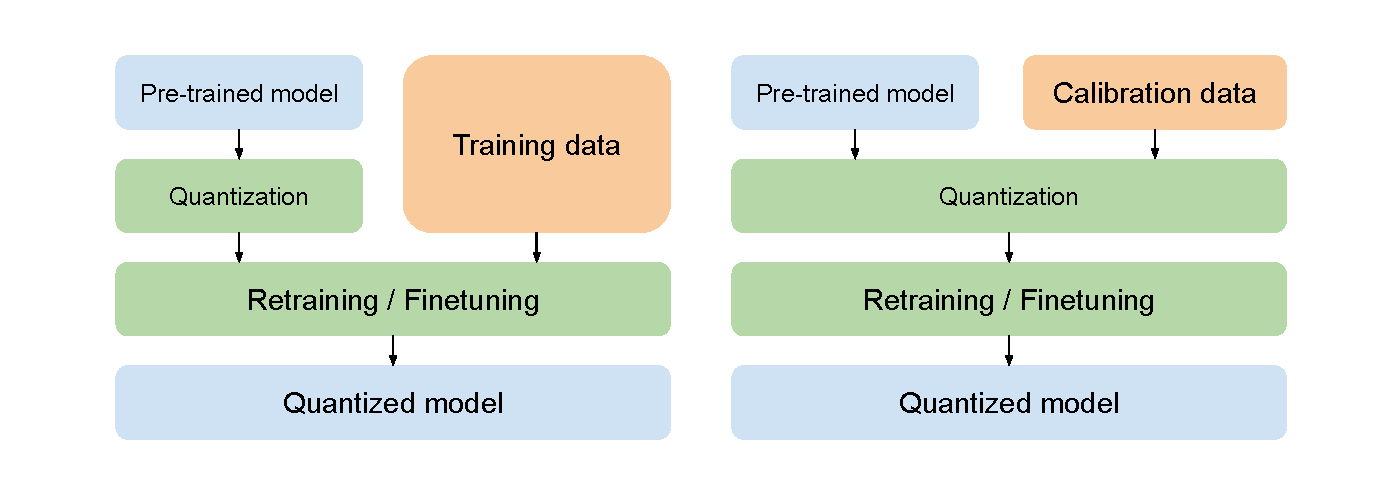
\includegraphics[width=0.85\textwidth]{pics/qat_ptq.pdf}
    \caption{Comparison between quantization-aware training (QAT, Left) and post-training quantization
    (PTQ, Right). In QAT, quantization is simulated during training or fine-tuning so that the model can
    adapt to low-precision weights and activations. In PTQ, a pretrained model is quantized after
    training, typically using a calibration dataset to determine quantization ranges and scaling
    factors. Cropped from Gholami et al.~\cite{gholami2022survey}.}
    \label{fig:qat_ptq_comparison}
\end{figure}

\paragraph{Simulated and integer-only quantization}
It is also important to distinguish simulated quantization from integer-only inference. In simulated
or fake quantization, tensors may be stored in low precision, but the actual arithmetic is still
performed in floating point after dequantization. This can reduce memory footprint, but it does
not fully exploit low-precision arithmetic units. In integer-only quantization, operations such as
convolution and matrix multiplication are performed using integer arithmetic, often with INT8
multiplication and INT32 accumulation. This is the form of quantization most relevant for
deployment on edge accelerators and mobile inference libraries, because it can reduce both memory
traffic and arithmetic cost. However, integer-only inference imposes stricter constraints on operator
support. Operations such as residual additions, normalization, softmax, GELU, or other nonlinear
functions may require special integer approximations, rescaling steps, or fallback to floating-point
execution. If unsupported operators fall back to floating point, the practical speedup can be much
smaller than expected.

\paragraph{Mixed precision}
Uniformly assigning the same low precision to every layer is often suboptimal. Different layers
have different sensitivity to quantization: some layers can be reduced to INT8, INT4, or even
lower precision with little loss, while others cause large accuracy degradation if quantized too
aggressively. Mixed-precision quantization assigns different bit widths to different layers or
operators. Sensitive layers are kept at higher precision, while less sensitive or more expensive
layers are quantized more aggressively. This can provide a better trade-off between accuracy,
latency, energy, and model size.

The main difficulty is that choosing the bit width of each layer creates a large combinatorial search
problem. For a network with $L$ layers and $k$ possible bit widths per layer, the number of
possible assignments is $k^L$. Existing methods therefore use heuristics, sensitivity analysis,
reinforcement learning, differentiable search, or hardware-aware optimization to choose the
precision configuration. The optimal assignment is also hardware-dependent: a lower bit width is
only useful if the target device and inference backend provide efficient kernels for that precision.
For example, INT8 may be well supported on CPUs and edge accelerators, while INT4 may require
specialized kernels or hardware support. Thus, mixed precision should be evaluated not only by
model accuracy, but also by real latency, memory bandwidth, and power consumption on the
target platform.

\paragraph{Summary}
Quantization reduces inference cost by replacing floating-point weights and activations with
lower-precision representations. Its practical effectiveness depends on several interacting design
choices: the quantization function, clipping range, calibration method, symmetric or asymmetric
mapping, quantization granularity, static or dynamic activation ranges, and whether inference is
simulated or integer-only. PTQ provides a simple and fast deployment path, but may reduce
accuracy, while QAT usually improves accuracy at the cost of retraining. Mixed precision further
extends this trade-off by assigning different bit widths to different layers according to their
sensitivity and hardware efficiency. Therefore, quantization should be understood not only as a
numerical compression method, but also as a hardware-aware deployment technique whose
benefits depend strongly on compiler support, backend kernels, and the target device.

\section{Pruning and Structural Simplification}

Pruning is a model-compression technique that reduces the number of parameters, filters,
channels, or other computational structures in a neural network after or during training. The
basic motivation is that modern deep neural networks are often over-parameterized: many weights
or channels can be removed with little effect on accuracy. A smaller network can reduce memory
usage, arithmetic cost, and energy consumption, which is especially relevant for deployment on
edge devices. However, the practical benefit of pruning depends strongly on the type of sparsity
introduced. Removing individual weights can produce a highly sparse model, but such
unstructured sparsity is difficult to accelerate on general-purpose CPUs and GPUs without
specialized sparse kernels or hardware support. In contrast, structured pruning removes entire
filters, channels, neurons, or blocks, producing dense smaller tensors that are easier for existing
compilers and inference runtimes to exploit.

Vadera and Ameen~\cite{vadera2022methods} categorize studies on neural-network pruning into
eight broad groups: magnitude-based pruning, similarity and clustering methods, sensitivity
analysis methods, knowledge distillation, low-rank methods, quantization methods, architectural
design methods, and hybrid methods. In a strict sense, not all of these are pruning methods.
Knowledge distillation, low-rank approximation, quantization, and architectural search are better
understood as related model-compression or model-efficiency techniques. Nevertheless, they are
often discussed together with pruning because they pursue the same goal: reducing the memory,
latency, or energy cost of neural-network deployment.

\paragraph{Magnitude-based pruning}
Magnitude-based pruning removes parameters or structures according to simple local measures,
most commonly the absolute value or norm of weights, filters, or activations. The intuition is that
weights or filters with small magnitude contribute less to the network output and can therefore be
removed. Early work by Han et al.~\cite{han2015learning} demonstrated that iterative magnitude
pruning followed by fine-tuning can remove a large fraction of weights from networks such as
LeNet, AlexNet, and VGG without significant loss in accuracy. Their results also showed two
important practical lessons: iterative pruning is usually more effective than one-shot pruning, and
fine-tuning the remaining weights is preferable to simply reinitializing the pruned network.

Later work observed that pure magnitude pruning can remove weights too early. Guo et al.\
introduced Dynamic Network Surgery~\cite{guo2016dynamic}, where pruned weights are not
permanently discarded but can be restored if they later become important. This addresses the
problem that the importance of a weight can change after other weights have been removed.

Magnitude-based pruning also extends naturally to structured pruning. Instead of removing
individual weights, a method can remove filters or channels whose norms are small. For example,
Li et al.~\cite{li2016pruning} prune convolutional filters based on the sum of absolute filter weights.
This form of pruning is more deployment-friendly than unstructured weight pruning because
removing an entire filter or channel reduces tensor dimensions and produces a smaller dense
network. Such structural changes are more likely to translate into real speedups in standard
deep-learning frameworks and compiler backends.

\paragraph{The lottery ticket hypothesis}
The Lottery Ticket Hypothesis introduced by Frankle and Carbin~\cite{frankle2018lottery}
reframed pruning as a way to identify trainable subnetworks inside a larger network. The
hypothesis states that a randomly initialized dense network contains a sparse subnetwork, a
``winning ticket'', that can be trained to match the accuracy of the original network in no more
training iterations than the full model. Their procedure uses magnitude pruning to identify the
subnetwork, resets the remaining weights to their initial values, and retrains.

This work is important because it suggests that pruning is not only a post-hoc compression
technique, but also a tool for studying over-parameterization and trainability. However, later
studies showed that the behavior depends on model size, dataset, pruning level, and whether the
remaining weights are reset to their original initialization or to a later training checkpoint. For
larger networks and harder datasets, resetting to later training iterations can be more stable than
resetting to the initial weights~\cite{frankle2019stabilizing}. From a deployment perspective, the
lottery-ticket literature is conceptually important, but its direct usefulness is limited unless the
resulting sparse subnetworks can be efficiently executed.

\paragraph{Structured channel and filter pruning}
Structured pruning removes complete channels, filters, neurons, or blocks. This is often more
important for real inference acceleration than unstructured sparsity. If an entire output channel is
removed from a convolutional layer, the corresponding input channel in the following layer can
also be removed. This reduces both the number of parameters and the number of dense
multiply--accumulate operations.

Vadera and Ameen~\cite{vadera2022methods} identify three main directions in structured channel
and filter pruning: data-dependent methods, data-independent methods, and optimization-based
channel approximation methods.

\subparagraph{Data-dependent channel pruning}
Data-dependent methods estimate the usefulness of a channel by observing its behavior on a
sample of input data. The underlying assumption is that an informative channel should respond
differently to different inputs. Polyak and Wolf~\cite{polyak2015channel} proposed pruning
methods based on feature-map variance. Channels or filters whose activations vary little across
samples are considered less informative and can be pruned. Their Reduce and Reuse method also
addresses a key difficulty in output-channel pruning: removed channels may still be expected by
subsequent layers. To compensate, removed channels are approximated as linear combinations of
the remaining channels, implemented using an additional $1 \times 1$ convolution.

Entropy-based pruning follows a similar idea but measures the information content of feature
maps rather than their variance. If a feature map has low entropy, it is assumed to carry less
discriminative information and its corresponding filter may be removed. Such methods can be
more meaningful than pure magnitude criteria, but they require representative data and additional
forward passes to estimate channel statistics.

\subparagraph{Data-independent channel pruning}
Data-independent methods use properties of the learned weights or activations without explicitly
solving a reconstruction problem. Hu et al.~\cite{hu2016network} introduced Average Percentage
of Zeros (APoZ), where filters producing many zero activations are considered weak and are
removed. This is motivated by ReLU-based networks, where inactive channels may contribute
little to the final prediction. After pruning, the network is fine-tuned to recover accuracy.

Another simple data-independent approach is filter-norm pruning, where filters with small
$\ell_1$ or $\ell_2$ norms are removed. These methods are attractive because they are cheap and
easy to implement. Their limitation is that small magnitude does not always imply low importance:
a filter can have small weights but still be useful, while a large filter may be redundant if its
function is duplicated by other filters.

\subparagraph{Optimization-based channel approximation}
Optimization-based channel pruning methods remove channels while explicitly trying to preserve
the layer output. Rather than asking which channels are individually small or inactive, these
methods ask which subset of channels best reconstructs the original feature maps. ThiNet
~\cite{luo2017thinet}, for example, formulates channel selection as an optimization problem and
uses a greedy strategy to choose channels whose removal minimally affects the next layer. After
the subset of channels is chosen, the remaining weights are re-optimized using least squares.

Related methods use LASSO regression or other approximations to select channels and refit the
remaining weights. These approaches are often more accurate than simple magnitude pruning
because they account for the interaction between channels. Their disadvantage is additional
computational cost: estimating reconstruction error and solving optimization problems requires
data samples and extra pruning-time computation.

\paragraph{Similarity and clustering methods}
Similarity and clustering methods remove redundant structures rather than individually weak
ones. The main assumption is that over-parameterized networks may contain filters or channels
that perform similar functions. If two filters are highly similar, one may be removed or replaced
with an approximation based on the other. Representative approaches include geometric median
filter pruning~\cite{he2019filter}, ThiNet~\cite{luo2017thinet}, and FilterSketch~\cite{lin2021filter}.

Geometric median pruning removes filters that are close to the geometric median of the filter set,
because such filters are assumed to contain information already represented by other filters.
FilterSketch instead aims to reduce the number of filters while preserving covariance information
among them. These methods are useful because they target redundancy directly. However, their
success depends on the assumption that similarity in weight or feature space corresponds to
functional redundancy, which may not always hold across architectures and tasks.

\paragraph{Sensitivity-analysis methods}
Sensitivity-analysis methods attempt to estimate the effect of removing a parameter, channel, or
filter on the loss function. These methods are more directly tied to the learning objective than
simple magnitude criteria. Classical examples include Optimal Brain Damage and Optimal Brain
Surgeon, which use second-order Taylor approximations of the loss to estimate weight saliency.
More recent methods use first-order or second-order approximations to prune channels and feature
maps in convolutional networks.

Taylor pruning~\cite{molchanov2016pruning} estimates the change in loss caused by removing a
feature map using a first-order Taylor approximation. SNIP~\cite{lee2018snip} performs
single-shot pruning before training by estimating the saliency of each connection at initialization.
GraSP~\cite{wang2020picking} instead aims to preserve gradient flow after pruning. These methods
can achieve strong accuracy--compression trade-offs because they prune according to estimated
task sensitivity. However, they are often more expensive than magnitude-based pruning and may
require gradient computation, data samples, or careful tuning.

\paragraph{Knowledge distillation and pruning}
Knowledge distillation is not pruning in the strict sense, because it does not necessarily remove
weights from an existing model. Instead, a large teacher model transfers predictive behavior to a
smaller student model~\cite{hinton2015distilling}. The student may be a manually designed compact
architecture, a pruned network, or a structurally simplified model. Distillation is especially useful
after structured pruning, because the pruned model can be trained to match the outputs or
intermediate representations of the original model. Methods such as discrimination-aware channel
pruning~\cite{zhuang2018discrimination} combine pruning with auxiliary losses to preserve
discriminative features.

The advantage of distillation is that it can recover accuracy that would otherwise be lost during
compression. The limitation is that it introduces additional training complexity and usually
requires access to training data and a strong teacher model. Therefore, distillation is powerful when
accuracy is critical, but less convenient for fast, hardware-agnostic compression.

\paragraph{Low-rank approximation, quantization, and architectural search}
Low-rank approximation, quantization, and architectural search are related to pruning but should
be treated as broader model-efficiency techniques. Low-rank methods factor large weight tensors
or matrices into smaller components, reducing computation in convolution-heavy models. Their
effectiveness depends on whether the learned weights admit a good low-rank approximation.
At high compression levels, accuracy may degrade quickly.

Quantization reduces numerical precision rather than removing structures. It is commonly
combined with pruning because the two methods attack different sources of cost: pruning reduces
the number of parameters or operations, while quantization reduces the cost of storing and
executing the remaining ones. Quantization-aware training~\cite{jacob2018quantization} and binary
or ternary networks such as XNOR-Net~\cite{rastegari2016xnor} are therefore better discussed as
complementary compression methods rather than pruning methods.

Architectural design methods, including NAS- and reinforcement-learning-based approaches such
as AMC, AutoSlim, and Once-for-All, search directly for efficient architectures. These methods may
produce networks that resemble pruned architectures, but they differ from classical pruning
because they optimize the architecture itself rather than removing parts from a fixed trained
network.

\paragraph{Deployment considerations}
The main practical distinction is between unstructured and structured pruning. Unstructured
pruning can remove a very large number of individual weights and therefore achieves high nominal
compression. However, unless the target hardware, compiler, and runtime support sparse tensor
operations efficiently, the model may not become faster. Sparse weight matrices can introduce
irregular memory access, index-storage overhead, and poor utilization of dense SIMD, GPU, or
NPU execution units.

Structured pruning is usually more useful for deployment because it changes tensor shapes and
reduces dense computation. Removing channels, filters, or blocks can reduce FLOPs and memory
traffic in a way that standard inference engines can exploit. This makes structured pruning more
relevant for compiler-aware model optimization, where the goal is not only to reduce the number
of parameters, but to produce a model that maps efficiently to the target backend. For edge
deployment, pruning should therefore be evaluated using real latency, memory consumption, and
power measurements, not only parameter count or theoretical FLOPs.

\paragraph{Summary}
Pruning methods differ in what they remove and how they estimate importance. Magnitude-based
methods are simple and cheap, but may remove parameters that are locally small yet globally
important. Sensitivity-analysis methods are more task-aware but computationally more expensive.
Similarity and clustering methods target redundancy between filters or channels, while
optimization-based methods explicitly preserve layer outputs after channel removal. For practical
deployment, structured pruning is generally more useful than unstructured pruning because it
produces smaller dense models that are easier for existing compilers, libraries, and hardware
backends to accelerate. In the context of this thesis, pruning is therefore most relevant when it
leads to structural simplification of the model, such as reducing channels, filters, or blocks in a
way that improves actual inference latency and energy efficiency on edge hardware.

% ======= Theory =======
\chapter{Theory}
\label{chap:literature}

\section{Metrics Description}


To evaluate the performance of object detection models, a set of standard metrics is used throughout this report.
These metrics assess both localization accuracy and classification quality, providing a comprehensive view of
model behavior.

\begin{itemize}[leftmargin=1.5em]

    \item \textbf{Intersection over Union (IoU)}:\\
    For a predicted bounding box \(p\) and a ground-truth box \(g\), the Intersection over Union is defined as:
    \[
        \IoU(p,g) = \frac{|p \cap g|}{|p \cup g|}.
    \]
    IoU measures localization accuracy by quantifying the overlap between predicted and ground-truth boxes.
    It is computed as the ratio of the intersection area to the union area of the two boxes, resulting in a value between 0 and 1.
    A score of 1 indicates perfect alignment, while 0 indicates no overlap.

    In practice, an \textit{IoU threshold} (e.g., 0.5) is used to determine whether a prediction is correct.
    Predictions with \(\IoU \geq \tau\) are considered true positives (TP), while those below the threshold are treated as false positives (FP).
    IoU serves as a fundamental building block for higher-level evaluation metrics such as precision, recall, and mAP.

    \item \textbf{Precision and Recall}:\\
    Precision and recall evaluate the quality of classification and detection results. Precision measures the proportion of correct positive predictions:
    \[
        \text{Precision} = \frac{\TP}{\TP + \FP}.
    \]
    Recall measures the proportion of correctly detected instances among all ground-truth objects:
    \[
        \text{Recall} = \frac{\TP}{\TP + \FN}.
    \]
    Here, TP, FP, TN, and FN denote true positive, false positive, true negative, and false negative predictions, respectively.
    Precision reflects the ability to avoid false detections, while recall captures the ability to detect all relevant objects.

    \item \textbf{Average Precision (AP)}:\\
    Average Precision summarizes the precision-recall trade-off by computing the area under the precision-recall (P--R) curve~\cite{Goodfellow2016}:
    \[
        \AP_{\tau} = \int_{0}^{1} p(r;\tau)\,dr.
    \]
    The P--R curve is constructed by varying the detection confidence threshold:
    \begin{itemize}[leftmargin=1.5em]
        \item Each detection is assigned a confidence score \(s \in [0,1]\).
        \item Detections are sorted in descending order of confidence.
        \item Predictions are progressively included, and precision and recall are recomputed.
        \item This process generates the precision-recall curve.
    \end{itemize}
    AP corresponds to the area under this curve and provides a single scalar measure of detection performance.

    \begin{figure}[H]
      \centering
      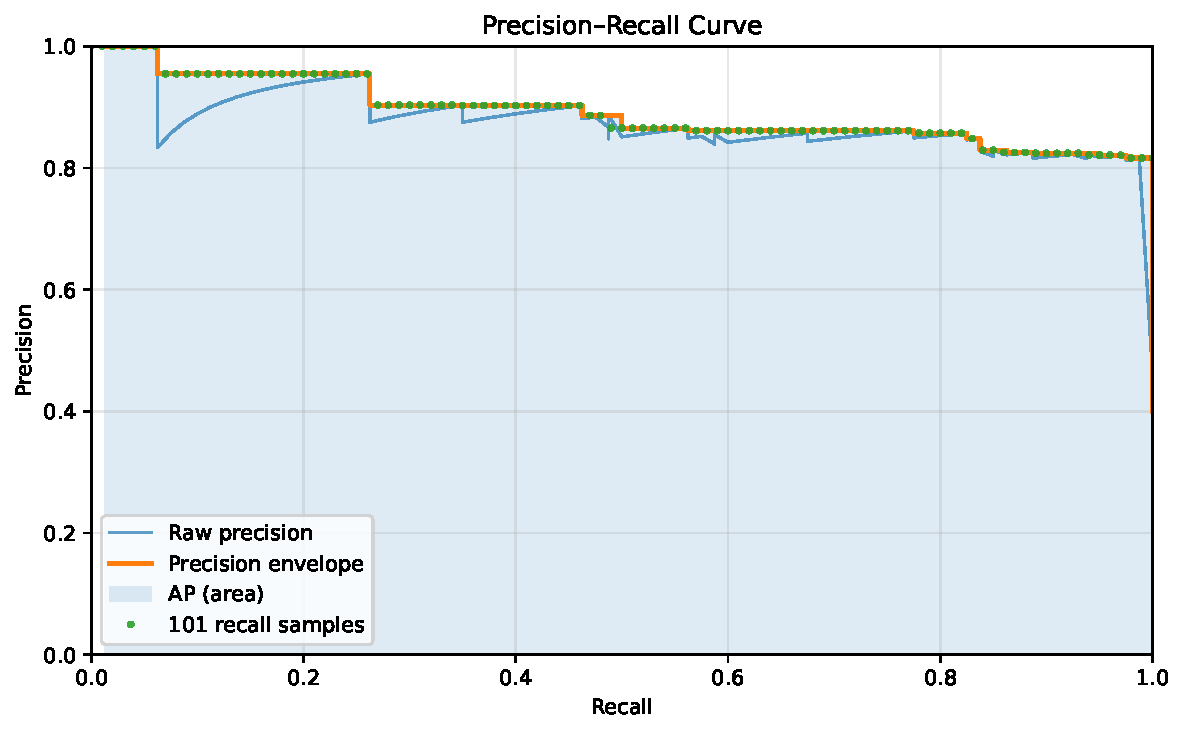
\includegraphics[width=0.8\linewidth]{pics/pr_concept.pdf}
      \caption{Precision--Recall curve.}
    \end{figure}

    \item \textbf{Mean Average Precision (mAP)}:\\
    Mean Average Precision extends AP to multi-class settings by averaging AP over all object classes:
    \[
        \mAP_{0.50} = \frac{1}{C} \sum_{c=1}^{C} \AP_{c,\,0.50},
    \]
    \[
        \mAP_{[0.50:0.95]} = \frac{1}{C} \sum_{c=1}^{C} \frac{1}{10}
        \sum_{k=0}^{9} \AP_{c,\,(0.50 + 0.05k)}.
    \]
    Here, \(C\) denotes the number of classes. The notation indicates the IoU threshold(s) used to determine true positives.
    For example, \(\mAP_{0.50}\) considers predictions with \(\IoU \geq 0.5\), while \(\mAP_{[0.50:0.95]}\) averages performance across multiple thresholds, providing a more comprehensive evaluation.

\end{itemize}

\section{Roofline Model Concept}

The Roofline model, introduced by Williams et al.~\cite{williams2009roofline},
provides an intuitive way to analyze whether a workload is limited by memory bandwidth
or computational throughput. It plots performance (e.g., Gigaflops per second (GFLOP/s)) versus arithmetic intensity
(FLOPs per byte of memory traffic). The model defines two limits: a sloped memory roof determined by peak memory
bandwidth, and a flat compute roof determined by peak floating-point throughput. Any kernel’s performance is
bounded by the minimum of these two ceilings. If a point lies on the sloped region, it is memory-bound;
if it lies on the flat region, it is compute-bound. The Roofline model is widely used to analyze whether a
workload  is limited by memory movement or computation and to guide optimization efforts.

Optimization strategy of a neural network model is dependent on whether our device limits us in the speed
of reading/writing to/from memory or the computational speed overall.

\begin{itemize}
    \item \textbf{If the workload is Memory-Bound:}\\
        This means performance is limited by memory bandwidth, not by compute units.
        The arithmetic intensity (FLOPs/byte) is low, so the kernel spends most of
        its time moving data.
        The goal is then to either increase arithmetic intensity, or reduce memory traffic.\\
        \textbf{Optimization strategies:}
        \begin{itemize}
            \item Improve data locality: reuse data in cashes (tiling/blocking);
            Keep tensors in shared memory (GPU);
            \item Fuse operations to avoid writing intermediate tensors to memory
            (Conv $\rightarrow$ BatchNorm $\rightarrow$ Silu) $\rightarrow$ (Fused Conv-BN-Activation)
            \item Reduce Precision (FP32 $\rightarrow$ FP16 $\rightarrow$ INT8 $\rightarrow$ INT4)
            \item Reduce tensor size: pruning, structured sparsity, channel reduction, smaller input resolution
            \item Improve memory layout: avoid unnecessary copies, channel-last format (NHWC)
        \end{itemize}
    \item \textbf{If the workload is Compute-Bound:}\\
        This means arithmetic units are saturated. Arithmetic intensity is high enough that bandwidth is no
        longer limiting. The goal is then to increase compute efficiency. This case is harder, as it requires
        the work with scheduling, parallelization, kernel optimization and algorithmic improvements. \\
\end{itemize}

    \begin{figure}[t]
        \centering
        \includegraphics[width=0.8\linewidth]{pics/roofline_model_custom.pdf}
        \caption{A Roofline model illustrating performance limits based on compute capability
            (horizontal line) and memory bandwidth (sloped line) versus the arithmetic intensity
            of operations (dots). Operations below the ``roof" are limited by either memory
            bandwidth or compute peak.}
        \label{fig:roofline}
    \end{figure}


    \begin{itemize}
        \item \textbf{Peak computational performance (in FLOP/s)} is obtained by benchmarking a compute-bound kernel that
        saturates the floating-point execution units.
        In practice, this can be achieved using large dense matrix multiplications
        of size $m \times k$ and $k \times n$, for which the floating-point operation count is given by:

            \begin{equation}
                \mathrm{FLOPs} = 2 \times m \times k \times n.
            \end{equation}

        The sustained peak performance is then computed as
            \begin{equation}
            P_{\mathrm{peak}} = \frac{\mathrm{FLOPs}}{t_{\mathrm{compute}}},
            \end{equation}
        where $t_{\mathrm{compute}}$ denotes the measured execution time.
        \item \textbf{Peak memory bandwidth (in GB/s)} is determined using a streaming memory
        benchmark. A large device-to-device copy or STREAM-like triad kernel is executed
        over a sufficiently large buffer to avoid cache effects. The sustained memory
        bandwidth is computed as
        \begin{equation}
        B_{\mathrm{peak}} = \frac{\mathrm{Bytes\ transferred}}{t_{\mathrm{memory}}}.
        \end{equation}
        \item \textbf{Arithmetic intensity (AI)} is defined as the ratio between the number of floating-point
        operations and the volume of data transferred to and from main memory:
        \begin{equation}
        \mathrm{AI} = \frac{\mathrm{FLOPs}}{\mathrm{Bytes}}.
        \end{equation}
        Since exact Dynamic Random-Access Memory (DRAM) traffic is generally unavailable without hardware performance counters, a lower-bound
        estimate of memory traffic is commonly used. For convolutional or linear layers, this lower bound
        consists of the input tensor, weight parameters, and output tensor:
        \begin{equation}
        \mathrm{Bytes}_{\mathrm{LB}} =
        \mathrm{Bytes}_{\mathrm{input}} +
        \mathrm{Bytes}_{\mathrm{weights}} +
        \mathrm{Bytes}_{\mathrm{output}}.
        \end{equation}
        This estimate ignores cache reuse and intermediate buffering, thereby providing an upper bound on
        arithmetic intensity.
        \item \textbf{The achieved performance of a workload} is computed as
        \begin{equation}
        P_{\mathrm{achieved}} = \frac{\mathrm{FLOPs}}{t_{\mathrm{execution}}}.
        \end{equation}
        The Roofline bound is then defined as
        \begin{equation}
        P_{\mathrm{roof}}(\mathrm{AI}) =
        \min \left( P_{\mathrm{peak}}, \; B_{\mathrm{peak}} \times \mathrm{AI} \right).
        \end{equation}

        If $P_{\mathrm{achieved}}$ approaches $B_{\mathrm{peak}} \times \mathrm{AI}$, the workload
        is memory-bound, if it approaches $P_{\mathrm{peak}}$, the workload is compute-bound.
        This methodology enables systematic classification of performance bottlenecks and guides
        optimization strategies such as improving data locality, increasing arithmetic intensity, or enhancing
        computational parallelism.
    \end{itemize}

\section{Activation Functions: ReLU and SiLU}

Activation functions play a critical role in introducing non-linearity into neural networks, enabling them to learn
complex representations. In this work, we consider two commonly used activation functions: Rectified Linear
Unit (ReLU) and Sigmoid Linear Unit (SiLU).

The ReLU activation function was introduced by \cite{nair2010relu} and is widely used due to its computational simplicity.
More recently, smooth activation functions such as SiLU (or Swish) \cite{ramachandran2017swish}
have been proposed, offering improved accuracy at the cost of increased computational complexity.

The ReLU activation is defined as:
\begin{equation}
\text{ReLU}(x) = \max(0, x)
\end{equation}
ReLU is computationally simple, requiring only a comparison and selection operation. This makes it highly efficient
on modern hardware, as it can be implemented with minimal arithmetic and memory overhead. Due to its simplicity,
ReLU is widely used in performance-critical applications and is well-supported by hardware accelerators.

In contrast, the SiLU activation (also known as the Swish function) is defined as:
\begin{equation}
\text{SiLU}(x) = x \cdot \sigma(x) = \frac{x}{1 + e^{-x}}
\end{equation}
where $\sigma(x)$ denotes the sigmoid function. Compared to ReLU, SiLU introduces additional non-linearity and has
been shown to improve model accuracy in many cases. However, it is computationally more expensive, as it requires
evaluation of the exponential function, a division, and a multiplication.

From a computational perspective, the key difference between the two functions lies in their complexity. ReLU involves
only a simple thresholding operation, which is typically memory-bound and incurs minimal computational cost. In
contrast, SiLU requires multiple floating-point operations, including transcendental functions, making it more
compute-intensive and potentially slower on hardware with limited support for such operations.

This difference has practical implications for model optimization. Replacing SiLU with ReLU can reduce inference
latency and improve hardware efficiency, especially on edge devices. However, this simplification may lead to a
degradation in model accuracy. Therefore, the choice of activation function represents a trade-off between
computational efficiency and predictive performance.

While smooth activation functions such as SiLU have been shown to improve accuracy, recent work suggests that simpler
functions like ReLU can offer advantages in terms of computational efficiency and activation
sparsity~\cite{mirzadeh2023relu}.
This sparsity can be exploited by hardware and compilers to reduce the number of
effective computations, leading to improved inference performance.

\chapter{Methodology}
\noindent

This chapter describes the experimental design and procedures used to evaluate inference optimization
of the YOLOv8n object detection model on two edge hardware platforms: the NVIDIA Jetson Orin Nano
(GPU-class edge accelerator) and the Raspberry Pi~5 (ARM CPU-class single-board computer).
The central research question is how different compiler-aware optimization strategies, spanning
framework selection, numerical precision, structural model simplification, and low-level kernel
customization, affect inference latency, energy consumption, and detection accuracy on
resource-constrained hardware.

The chapter covers model selection and justification, hardware and software platform configuration,
baseline establishment, bottleneck characterization via Roofline analysis and profiling, and the
design of each optimization experiment.
The evaluated backends include TensorRT, Apache TVM with MetaSchedule auto-tuning, ONNX Runtime,
and LiteRT (formerly TensorFlow Lite), applied at FP32, FP16, and INT8 precision where supported
by the target platform.

\section{Specification of the Scientific Work}

The Experimental Evaluation chapter is organized as a progressive sequence of optimization steps applied
to the YOLOv8n model across two target platforms: the Jetson Orin Nano GPU and the Raspberry Pi~5 CPU.

The experiments begin with a Roofline analysis, which characterizes the computational and memory
bandwidth limits of each platform and determines whether the unoptimized model is bottlenecked by
arithmetic throughput or memory access.
This establishes a theoretical bound on achievable inference performance and motivates the subsequent
optimization directions.

The second stage compares inference compiler performance in FP32 precision.
TensorRT, ONNX Runtime, and Apache TVM are evaluated on both platforms.
For TVM, this includes a full MetaSchedule auto-tuning campaign to ensure that measured latency
reflects hardware-optimized kernel implementations rather than generic fallback schedules.
Nsight Systems profiling is used to decompose GPU execution time by kernel category, revealing which
compilation and scheduling strategies account for performance differences between frameworks.

Precision reduction is then evaluated as a standalone optimization axis.
FP16 and INT8 inference are measured for all applicable backends, with INT8 quantization performed
using post-training calibration on a representative subset of the COCO training data.
Results are reported not only in terms of latency but also in terms of detection accuracy (mAP) and
power consumption, capturing the full accuracy--efficiency--energy trade-off.

The fourth stage evaluates structural pruning of the model.
A channel-level sensitivity analysis is performed to determine which layers tolerate channel reduction
without disproportionate accuracy loss, followed by a full-model pruning experiment to quantify the
achievable speedup from structural simplification.

The fifth stage investigates whether manually replacing a bottleneck subgraph with a custom TensorRT
plugin can reduce the overhead identified during profiling.
The C2f block at model layer~2 is reimplemented as a hand-written cuDNN-based plugin, and the
resulting latency and kernel execution profile are compared against the standard TensorRT engine.

Finally, the effect of activation function choice is examined.
SiLU activations are replaced with ReLU across the full model, and the impact on fusion quality,
latency, and detection accuracy is evaluated across all backends and both platforms.



\section{Model Selection}

YOLOv8n is selected as the reference model for this study. The model represents a practical and relevant target for
edge deployment because it combines a compact architecture with competitive detection accuracy. It is widely used in
real-world object detection tasks, is actively supported by the research and engineering community, and can be
exported to multiple deployment backends. These properties make it suitable for comparative analysis across inference
frameworks.

From a methodological perspective, YOLOv8n is large enough to expose non-trivial optimization challenges, including
operator fusion, memory movement overhead, kernel launch inefficiencies, and sensitivity to reduced precision. At the
same time, it remains sufficiently lightweight to allow repeated experimentation, retraining, export, and validation
on commonly available development hardware. This enables a controlled and reproducible study of both high-level and
low-level optimization strategies.

\section{Overall Experimental Procedure}

The experimental workflow follows five main stages:

\begin{enumerate}
    \item Establish a baseline using the original FP32 PyTorch model.
    \item Identify performance bottlenecks through roofline analysis and runtime profiling.
    \item Apply optimization techniques at the framework, numerical, and architectural levels.
    \item Evaluate the optimized models on target hardware using identical benchmarking conditions.
    \item Compare the resulting variants in terms of latency, throughput, and accuracy.
\end{enumerate}

This procedure ensures that each optimization step is assessed relative to a common reference and that conclusions are
based on measurable changes in both performance and predictive quality.

\section{Baseline Establishment}

The starting point of the study is the pretrained FP32 YOLOv8n model provided by Ultralytics and executed in the
original PyTorch runtime. This baseline serves two purposes. First, it provides a reference for all later comparisons.
Second, it makes it possible to determine whether the observed performance is already close to the limits of the target
hardware or whether substantial optimization opportunities remain.

The baseline is evaluated on the selected hardware platforms under controlled conditions. For each platform, inference
latency and throughput are measured using repeated runs with warm-up iterations to reduce initialization effects.
Accuracy is evaluated on the validation dataset using standard object detection metrics. These baseline results form
the reference against which all optimized variants are compared.

\section{Bottleneck Analysis}

After establishing the baseline, the next step is to determine the dominant performance limitations of the model on
each platform. Two complementary approaches are used for this purpose: roofline-based reasoning and runtime profiling.

The roofline model is used as a coarse analytical framework to determine whether performance is likely to be limited
by memory bandwidth or by available compute throughput. This provides a hardware-aware interpretation of the measured
performance and helps identify whether the main limitation arises from insufficient arithmetic intensity, inefficient
memory access, or underutilization of the compute units.

To refine this analysis, profiling tools are used to inspect the execution of individual operators and kernels. This
makes it possible to identify layers with high latency, excessive memory movement, frequent kernel launches, or
inefficient execution patterns. In particular, the profiling stage is used to answer the following questions:

\begin{itemize}
    \item Which layers dominate end-to-end inference time?
    \item Whether the execution is primarily memory-bound or compute-bound.
    \item Whether the framework introduces avoidable overhead through layout conversions, intermediate buffers, or
    host-device synchronization.
    \item Whether operator fusion and backend-specific optimizations are effectively applied.
\end{itemize}

The outcome of this stage determines which optimization direction is most relevant for a given backend and hardware target.

\section{Optimization Directions}

Based on the bottleneck analysis, the study investigates several classes of optimization methods.

\subsection{Compiler and Runtime Optimization}

The first optimization direction consists of evaluating how different inference frameworks transform and execute the
same model. Starting from the original PyTorch implementation, the model is exported or compiled for alternative
backends such as TensorRT and TVM. The purpose of this comparison is to assess how much performance can be gained
from compiler-level graph transformations, backend-specific kernel selection, operator fusion, and scheduling
optimizations.

This stage is not limited to reporting end-to-end latency. It also examines how the internal execution differs between
backends, for example in the number of kernels launched, the use of fused operators, the presence of data layout
transformations, and the distribution of execution time across layers. In this way, the comparison provides insight
not only into which backend is faster, but also into why it is faster.

\subsection{Numerical Precision Reduction}

The second optimization direction focuses on reducing numerical precision in order to decrease memory traffic and
accelerate arithmetic operations. Two forms of precision reduction are considered in this work.

First, inference in FP16 is evaluated against the FP32 baseline. This comparison isolates the effect of reduced
floating-point precision and shows whether the target hardware benefits from half-precision execution. This step is
performed through ONNX Framework. It provides a dedicated conversion utility, that transforms a floating-point model
into a half-precision one without retraining. The converter traverses every node and tensor initializer in the graph:
weight tensors stored as \path{float32} NumPy arrays are recast to \path{float16} in place, and constant nodes are
rewritten to carry 16-bit values. Where the original graph boundary expects 32-bit input or produces 32-bit output,
explicit \path{Cast} nodes are inserted to handle the precision transition transparently. Certain operators whose
numerical stability is sensitive to reduced range, such as \path{LayerNormalization} or some reduction ops, can be
placed on a blocklist; the converter keeps those nodes in \path{float32} and surrounds them with \path{Cast} nodes
so the rest of the graph remains in FP16. The result is a structurally identical ONNX graph in which most weights,
activations, and intermediate tensors occupy half the memory and can be executed with FP16 arithmetic on any backend
that supports it, including TensorRT and ONNX Runtime with CUDA execution provider.

Second, quantization to INT8 is explored where supported by the backend. Quantization has the potential to reduce model
size, memory bandwidth requirements, and arithmetic cost, but it may also introduce accuracy degradation. Therefore,
each quantized model is evaluated not only in terms of runtime performance but also in terms of detection quality. The
purpose of this stage is to determine whether the performance gains justify the loss, if any, in predictive accuracy.
Quantization is explored via framework, which actively support it. Reducing precision from \path{float32} to
\path{int8} is more involved than the FP16 cast because 8-bit integers cannot represent the same dynamic range as
floating-point values. The mapping requires a learned scale factor and a zero point per tensor, so that
a floating-point value is approximated as:

\begin{equation}
    x \approx s \cdot (x_{\mathrm{int8}} - z), \quad x_{\mathrm{int8}} = \mathrm{clamp}\!\left(\left\lfloor \frac{x}{s}
    \right\rceil + z,\; -128,\; 127\right)
\end{equation}

The scale and zero point are not free parameters, and they must be determined from the actual distribution
of values the tensor takes during inference.
This calibration step was performed by gathering and running a small representative dataset through the unquantized
network and collecting per-tensor activation statistics.
Weights are quantized per-channel (one scale per output channel) to preserve accuracy;
activations are quantized per-tensor for runtime efficiency, but it can vary by the choice made by framework developers
and chosen setting. The calibration dataset was drawn from the COCO training split, the same distribution on which
YOLOv8n was originally trained.
Three subset sizes were evaluated: 0.1\%, 1\%, and 10\% of the training set, corresponding to approximately 118, 1,180,
and 11,800 images respectively. The 1\% subset was used as the primary calibration set throughout the report, in line
with framework documentation recommendations and confirmed by preliminary accuracy tests.
Subset size mainly affects the accuracy of the post-quantization network: a larger set provides a more faithful estimate
of the activation distribution, while a smaller set reduces calibration time with diminishing accuracy cost beyond a
certain threshold.
The 1\% subset was found to represent the activation distribution sufficiently for the purposes of this evaluation.

\subsection{Model Compression and Structural Simplification}

The third optimization direction targets the structure of the model itself. Rather than relying only on framework-level
improvements, this part of the study investigates whether the network can be simplified in ways that improve runtime
characteristics.

Pruning approach used in experiments was implemented in \texttt{manual\_yolov8\_pruner.py}, it performs targeted
structural pruning directly on the YOLOv8n PyTorch model graph.
The script accepts an explicit list of layer targets (e.g.\ \texttt{model.2.cv1},
\texttt{model.4.m.0.cv2}) and applies output-channel pruning to each nominated convolutional block.
Channel importance is estimated by the L2 norm of each output filter:
\begin{equation}
s_k = \left\lVert W_{k,:,:,:} \right\rVert_2, \quad k = 1, \ldots, C_{\mathrm{out}}
\end{equation}
where $W_k$ is the k-th output filter of the convolution weight tensor.
The top- $\lfloor(1-r)\cdot C_{\mathrm{out}}\rceil$ channels ranked by this score are retained, with
r being the per-block prune ratio and an optional rounding constraint (e.g.\ to a multiple of 8
for hardware alignment).
After each selected block is pruned, the script performs a full graph realignment pass: it propagates
the updated channel indices through all downstream consumers, slicing input weight matrices accordingly
and handling Concat, Upsample, and Detect nodes transparently.
Special handlers manage the internal structure of C2f blocks (cv1 hidden dimension, bottleneck cv1 and
cv2 paths) and the SPPF hidden channels.
The pruned model is saved as a \texttt{.pt} checkpoint suitable for fine-tuning and subsequent ONNX
export.
The other researched optimization is a replacement of computationally expensive operations with simpler alternatives.
In particular, the effect of replacing SiLU activations with ReLU is evaluated. This substitution is motivated by the
fact that simpler activations may improve fusion opportunities and reduce kernel complexity, even if they slightly
affect model accuracy. The SiLU activation substitution is applied directly to the PyTorch module tree before the model is
exported to ONNX.
Every \path{Conv} wrapper in the Ultralytics model carries an \path{.act} attribute; by iterating
over all named modules and replacing each \path{nn.SiLU()} instance with \path{nn.ReLU()}, the
entire network is converted in-place without altering any weight tensors.
The modified model is then saved as a \path{.pt} file and passed to the standard Ultralytics
\path{model.export(format="onnx")} pipeline.
Because the substitution happens at the PyTorch level, the resulting ONNX graph contains \path{Relu}
nodes in all positions where \path{Sigmoid}–\path{Mul} pairs (the ONNX decomposition of SiLU) would
otherwise appear, allowing downstream compilers and runtimes to fuse the activation with the preceding
convolution more readily.

The purpose of this stage is to understand whether modest architectural simplifications can produce a favorable
trade-off between accuracy and efficiency, especially on hardware with limited compute capability or reduced support
for complex fused kernels.

\subsection{Low-Level TensorRT Customization}

The final optimization direction extends beyond standard framework usage and examines low-level customization within
TensorRT. In this stage, custom plugins are developed to replace selected subgraphs with tailored implementations. The
main case considered in this work is a custom plugin for the C2f block.

The objective of this step is to investigate whether performance can be improved further by reducing backend overhead,
controlling kernel behavior more explicitly, or eliminating inefficient execution patterns that are not resolved by the
default TensorRT conversion pipeline. This stage complements the framework-level comparison by showing the extent to
which manual low-level intervention can outperform standard automated optimization.

This optimization is discussed in more details in the corresponding results section.

\section{Evaluation Criteria}

All model variants are evaluated using the same set of criteria in order to ensure consistent comparison.

The primary performance metrics are inference latency and throughput. Latency is used to measure the response time of
a single inference pass, while throughput indicates the sustained processing rate under repeated execution. Where
relevant, profiling data is also used to analyze kernel-level execution time and the contribution of individual
layers to the total runtime.

The primary quality metric is object detection accuracy on the validation dataset. Standard detection metrics are
used to verify whether a given optimization preserves acceptable predictive performance. This is particularly important
for quantization, pruning, and activation replacement, where improvements in runtime may come at the cost of degraded
detection quality.

The final analysis therefore considers both efficiency and accuracy, with emphasis on the trade-off between them. An
optimization is not treated as beneficial solely because it accelerates execution; it must also maintain sufficient
model quality for practical deployment.

\section{Methodological Summary}

The methodology combines baseline benchmarking, bottleneck analysis, framework comparison, numerical optimization,
structural simplification, and low-level backend customization. The goal is not only to identify the fastest deployment
configuration for YOLOv8n, but also to understand which classes of optimization are most effective on edge-oriented
hardware and under which conditions they provide measurable benefit.

The full implementation, including pruning scripts, quantization pipelines, TVM compilation workflows, and the custom
TensorRT plugin, is available as an open-source repository~\cite{bukueva2026thesis}.

Figure~\ref{fig:thesis_scope} summarizes the scope of the study and the main experimental directions considered in
this thesis.

\begin{figure}[ht]
\centering
\resizebox{\textwidth}{!}{%
\begin{tikzpicture}[
    font=\small,
    every node/.style={align=center},
    box/.style={
        rectangle,
        draw=black,
        text width=3.2cm,
        minimum height=1.0cm,
        inner sep=4pt
    },
    line/.style={draw, thick},
    boxsmall/.style={
    rectangle,
    draw=black,
    text width=2.2cm,
    minimum height=1.0cm,
    inner sep=4pt
    },
]

% Top node
\node[box] (scope) at (0,0) {Research Scope};

% First level
\node[box] (comp) at (-6,-2.2) {Compiler / Runtime\\Optimization};
\node[box] (eff)  at (0,-2.2)  {Model Compression\\and Efficiency};
\node[box] (prec) at (6,-2.2)  {Numerical Precision\\and Quantization};

% Second level
\node[box] (tvm)   at (-8,-4.4) {TVM Compilation\\Analysis};
\node[box] (trt)   at (-4,-4.4) {TensorRT Analysis};

\node[box] (prune) at (0,-4.4)  {Pruning};

\node[box] (quant) at (4,-4.4)  {Quantization};
\node[box] (fp16)  at (8,-4.4)  {FP32 vs FP16};

% Third level under TensorRT
\node[box] (plugin) at (-6,-6.6) {Custom\\C2f Plugin};
\node[box] (relu)   at (-2,-6.6) {ReLU vs SiLU};

% Connections
\draw[line] (scope.south) -- +(0,-0.5) -| (comp.north);
\draw[line] (scope.south) -- +(0,-0.5) -- (eff.north);
\draw[line] (scope.south) -- +(0,-0.5) -| (prec.north);

\draw[line] (comp.south) -- +(0,-0.5) -| (tvm.north);
\draw[line] (comp.south) -- +(0,-0.5) -| (trt.north);

\draw[line] (eff.south) -- (prune.north);

\draw[line] (prec.south) -- +(0,-0.5) -| (quant.north);
\draw[line] (prec.south) -- +(0,-0.5) -| (fp16.north);

\draw[line] (trt.south) -- +(0,-0.5) -| (plugin.north);
\draw[line] (trt.south) -- +(0,-0.5) -| (relu.north);

\end{tikzpicture}%
}
\caption{Overview of the thesis scope and main experimental directions.}
\label{fig:thesis_scope}
\end{figure}

% ======= 6 Testing / Results (Vår uttesting / Resultater) =======
\chapter{Experimental Evaluation}
\noindent

%\textcolor{red}{This chapter is currently in draft form and requires further structuring,
%    formatting, and completion of the subsections: c2f-plugin, relu\_silu activation functions substitution and prunning.
%    Its final revision is planned for the concluding phase of the thesis work.}

\section{Experimental Setup}

The experimental evaluation is conducted on two edge-oriented target platforms: the NVIDIA Jetson Orin Nano and the
Raspberry Pi 5. These devices represent two different deployment scenarios for embedded inference: a GPU-accelerated
AI platform with dedicated support for mixed-precision computation, and a general-purpose low-power ARM platform
without a dedicated on-chip neural network accelerator.

Model training, export, and selected modification experiments, such as pruning and operator substitution, are performed
on a host workstation equipped with an NVIDIA GeForce RTX 3070 GPU. This system is used as the primary development
and experimentation environment, while all deployment-oriented inference benchmarks are executed on the target edge
devices.

The Jetson Orin Nano is designed for edge AI and robotics workloads. Its system-on-chip integrates a 6-core Arm CPU,
an Ampere-based GPU, and shared LPDDR5 memory accessible by both CPU and GPU. This architecture is particularly
relevant for this study because it supports CUDA execution, Tensor Cores, mixed-precision inference, and INT8
acceleration, making it suitable for evaluating framework-level and low-level optimization strategies.

In contrast, the Raspberry Pi 5 represents a resource-constrained edge platform without a comparable integrated AI
accelerator. It is therefore used to assess how optimization techniques behave on a more conventional embedded
CPU-based system, where memory bandwidth and general-purpose compute resources are more limited.

Only the hardware characteristics most relevant to performance analysis are reported in this section, namely compute
capability, memory capacity, and memory bandwidth.

\begin{table}[H]
\centering
\caption{Host GPU specifications used for training and model development}
\label{tab:gpu_specs}
\begin{tabular}{@{}ll@{}}
\toprule
\textbf{Property} & \textbf{Value} \\
\midrule
Device            & NVIDIA GeForce RTX 3070 \\
Architecture      & Ampere \\
FP32 Performance  & $\sim$20 TFLOPs \\
Memory            & 8 GB GDDR6 \\
Memory Bandwidth  & $\sim$448 GB/s \\
\bottomrule
\end{tabular}
\end{table}

\begin{table}[H]
\centering
\caption{Specifications of the target edge devices}
\label{tab:edge_specs}
\begin{tabular}{@{}lll@{}}
\toprule
\textbf{Property} & \textbf{Jetson Orin Nano} & \textbf{Raspberry Pi 5} \\
\midrule
CPU              & 6-core Arm Cortex-A78AE   & 4-core Arm Cortex-A76 \\
GPU              & Ampere (1024 CUDA cores)  & VideoCore VII \\
FP32 Performance & $\sim$0.5--1 TFLOPs (GPU) & --- \\
Memory           & 8 GB LPDDR5               & 8 GB LPDDR4X \\
Memory Bandwidth & $\sim$102 GB/s             & $\sim$17 GB/s \\
Accelerators     & Tensor Cores              & None$^{*}$ \\
\bottomrule
\end{tabular}

\vspace{0.5em}
\raggedright
{\footnotesize
$^{*}$ The Raspberry Pi 5 can be extended with external AI accelerators, such as the Hailo-8, via PCIe. However,
    such accelerators are not used in the experiments reported in this thesis.
}
\end{table}


\section{Roofline Model}
\label{sec:roofline_analysis}

Constructing an accurate Roofline model for real-world workloads presents several challenges.
First, the performance characteristics reported by hardware manufacturers often differ from
measured values under practical conditions. Second, the effective behavior of a model depends
on the execution framework, including factors such as cache utilization, memory reuse, and
implicit optimizations (e.g., operator fusion), which are typically not visible at the model level.

Official YOLOv8 model characteristics are summarized in Table~\ref{tab:yolov8_models}.
The smallest variant, YOLOv8n, contains 3.2M parameters and requires 8.7B floating-point operations
for a single forward pass at 640$\times$640 resolution.

\begin{table}[ht]
\centering
\caption{Comparison of YOLO models (trained on COCO) at 640$\times$640 resolution~\cite{ultralytics_yolov8_performance}.}
\label{tab:yolov8_models}
\begin{tabular}{lcccc}
\toprule
Model &
CPU ONNX (ms) & A100 TensorRT (ms) & Params (M) & FLOPs (B) \\
\midrule
v8n & 80.4  & 0.99 & 3.2  & 8.7   \\
v8s & 128.4 & 1.20 & 11.2 & 28.6  \\
v8m & 234.7 & 1.83 & 25.9 & 78.9  \\
v8l & 375.2 & 2.39 & 43.7 & 165.2 \\
v8x & 479.1 & 3.53 & 68.2 & 257.8 \\
\bottomrule
\end{tabular}
\end{table}

While vendor specifications indicate that the Raspberry Pi 5 provides up to 17\,GB/s of memory bandwidth~\cite{raspberrypi_processors},
and the Jetson Orin Nano offers up to 102\,GB/s~\cite{nvidia_jetson_orin_datasheet},
measured performance is often significantly lower in practice.

\subsection{Roofline Analysis on Raspberry Pi 5}

Using the methodology described in Chapter~\ref{chap:literature}, the sustained memory bandwidth of the Raspberry Pi 5
was measured at 5.67\,GB/s, and peak compute throughput at 73.95\,GFLOP/s.
All measurements were obtained with PyTorch configured to use 4 CPU threads, and layer timings
were reported as the median over 20 runs after warmup.

\noindent These values define the device Roofline:
\[
P(I) = \min\left(73.95,\; 5.67 \cdot I\right),
\]
with a ridge point at approximately 13.04 FLOPs/byte, separating memory-bound and compute-bound regimes.

Table~\ref{tab:roofline_pi5_layers} summarizes representative per-layer performance characteristics
of YOLOv8n executed on the Raspberry Pi 5 CPU using eager-mode PyTorch.

Layers with relatively low arithmetic intensity (AI $\approx$ 7--10 FLOPs/byte) achieve only modest
throughput, typically in the range of 4.8--8.0\,GFLOP/s, indicating memory-bound or memory-sensitive
behavior under the measured Roofline parameters. In contrast, deeper convolutional layers with higher
arithmetic intensity (AI $>$ 70 FLOPs/byte) achieve substantially higher effective throughput, often in
the range of 40--60\,GFLOP/s. Some layers with very high arithmetic intensity exceed 50\,GFLOP/s, showing
that smaller deep feature maps benefit from improved locality and higher compute utilization.

The distribution focal loss (DFL) convolution in the detection head has extremely low arithmetic
intensity (0.47 FLOPs/byte) and achieves only 0.6\,GFLOP/s, confirming strong memory limitation.

\begin{table}[ht]
\centering
\caption{Per-layer performance statistics of YOLOv8n on Raspberry Pi 5 (CPU, FP32).}
\label{tab:roofline_pi5_layers}
\begin{tabularx}{\textwidth}{l c c c X}
\toprule
Layer & Time (ms) & AI (FLOPs/byte) & Perf (GFLOP/s) & Regime \\
\midrule
0.conv              & 18.39 & 7.71   & 4.8  & Memory-bound \\
2.cv1.conv          & 8.84  & 7.99   & 5.9  & Memory-bound \\
2.cv2.conv          & 9.84  & 9.59   & 8.0  & Memory-bound \\
4.m.0.cv2.conv      & 2.74  & 70.42  & 43.1 & Compute-favored \\
6.m.1.cv2.conv      & 1.93  & 122.03 & 61.1 & Compute-favored \\
18.m.0.cv2.conv     & 2.02  & 122.03 & 58.5 & Compute-favored \\
22.cv3.0.1.conv     & 13.53 & 170.41 & 54.5 & Compute-favored \\
22.dfl.conv         & 1.89  & 0.47   & 0.6  & Strongly memory-bound \\
\midrule
Full Model          & 327.00 & 157.76 & 13.54 & Mixed / overhead-dominated \\
\bottomrule
\end{tabularx}
\end{table}

\begin{figure}[!h]
    \centering
    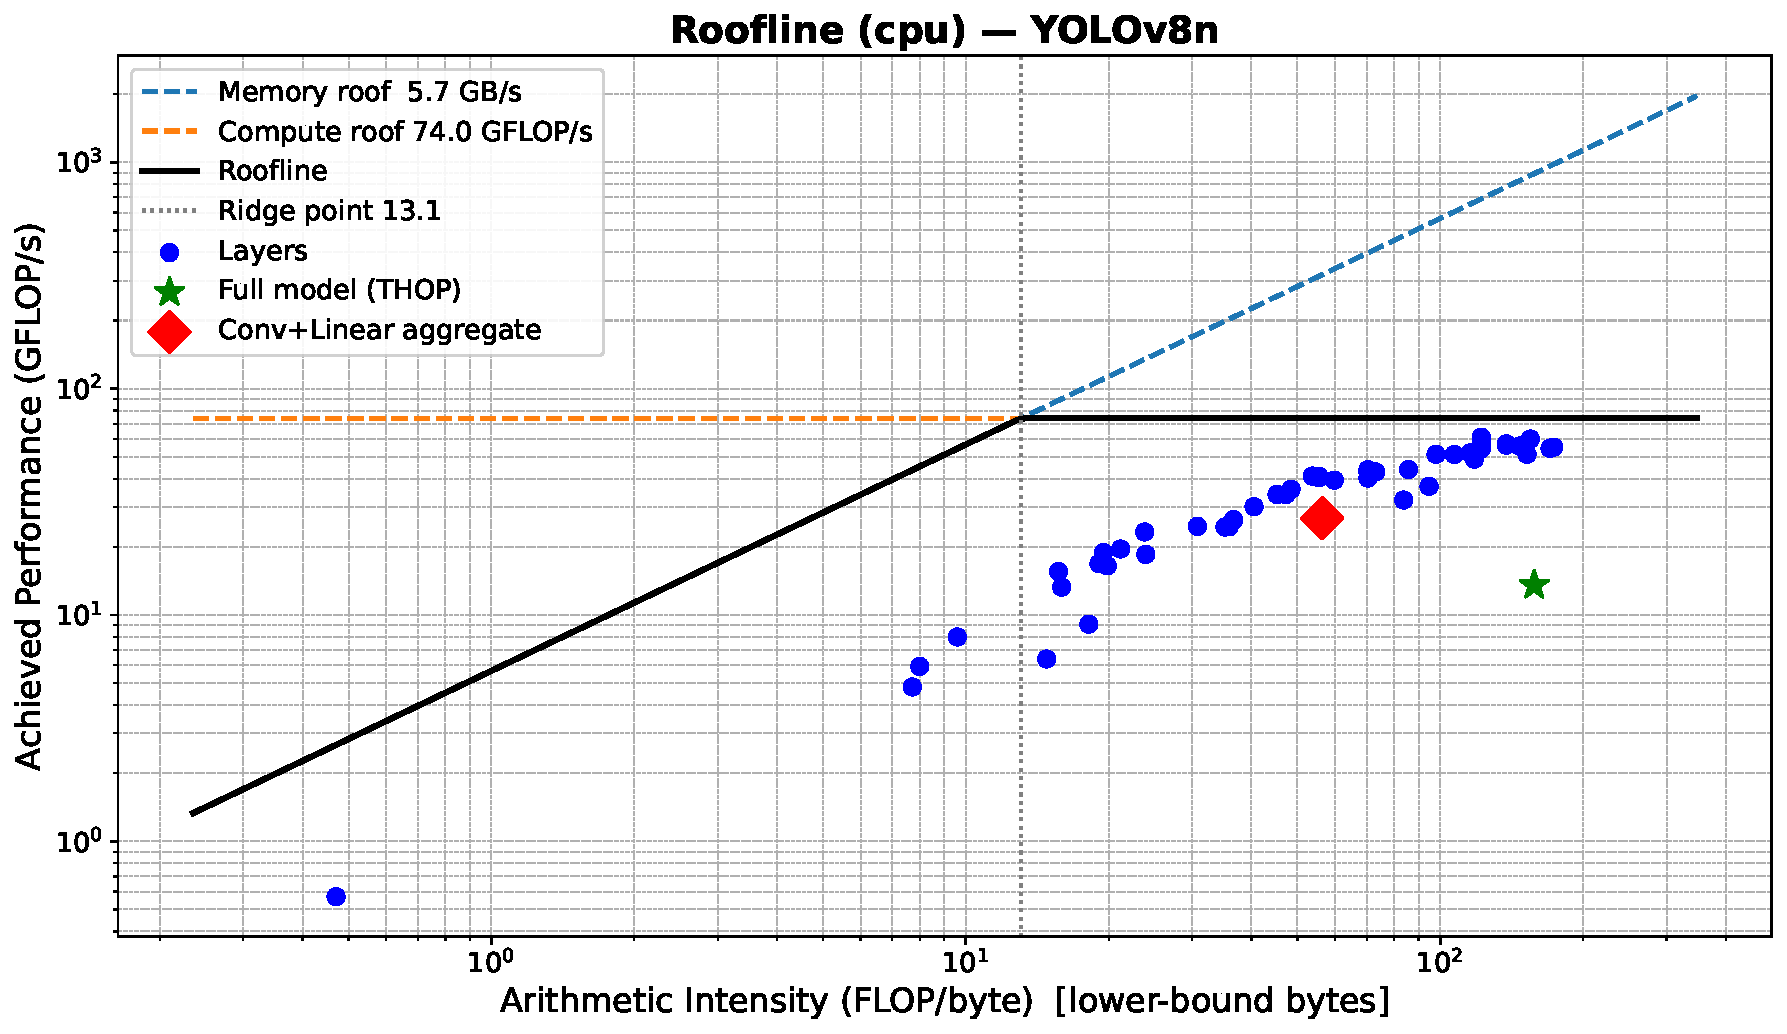
\includegraphics[width=0.8\linewidth]{pics/roofline_pi5_cpu_20260402_164102.pdf}
    \caption{Roofline model of YOLOv8n on Raspberry Pi 5 (CPU, FP32).}
    \label{fig:roofline_pi5}
\end{figure}

Although several individual convolutional layers exhibit relatively high effective throughput,
the overall model achieves only 13.54\,GFLOP/s, corresponding to approximately 18.3\% of the
measured device-level peak compute throughput of 73.95\,GFLOP/s.

This discrepancy indicates that end-to-end inference performance is not determined solely by the
efficiency of individual convolution kernels. Instead, it is also affected by system-level and
framework-level overheads, including kernel dispatch overhead, synchronization, non-convolutional
operations, tensor reshaping and concatenation, inter-layer memory traffic, and limited fusion
between adjacent operators. Thus, the Roofline serves primarily as an upper bound and an interpretive
tool rather than a directly attainable end-to-end target.

From an optimization perspective, these results suggest that further improvements should focus not
only on reducing memory traffic, but also on improving execution efficiency at the graph and kernel
level. Promising directions include operator fusion, graph-level optimization, backend-specific kernel
tuning, quantization, and reducing framework overhead through more optimized runtimes.

\noindent The observed performance behavior can be further explained by the relationship between
layer activation sizes and the cache hierarchy:

\begin{itemize}
    \item L1: 64 KB per core
    \item L2: 512 KB per core
    \item L3: 2 MB shared
    \item DRAM bandwidth: $\approx$ 5.67 GB/s (measured)
\end{itemize}

In particular, the shared L3 cache of the Raspberry Pi 5 is limited to 2\,MB, which constrains
the amount of feature-map data that can be reused without returning to main memory.

Early layers of YOLOv8n operate on high-resolution feature maps (e.g., 320$\times$320),
resulting in activation tensors that far exceed the available cache capacity.
Consequently, these layers experience frequent DRAM accesses and comparatively low effective performance,
which is consistent with their lower arithmetic intensity and more memory-bound behavior.

In contrast, deeper layers operate on progressively smaller feature maps (e.g., 40$\times$40
or 20$\times$20), allowing a larger fraction of their working set to remain in cache.
This improves locality and data reuse, enabling substantially higher effective throughput.
Thus, even though the full model remains far below the ideal Roofline bound, the layerwise results
still reveal a clear transition from memory-bound early layers to more compute-favored deeper layers.

\subsection{Roofline Analysis on Jetson Orin Nano}

The same analysis was performed on the NVIDIA Jetson Orin Nano GPU.
With PyTorch configured to use a single host thread and using median timings
after warmup, the measured sustained memory bandwidth was 55.68\,GB/s,
while peak compute throughput reached 810.68\,GFLOP/s.

\noindent The resulting Roofline model is defined as:
\[
P(I) = \min\left(810.68,\; 55.68 \cdot I\right),
\]
with a ridge point at:
\[
I^* = \frac{810.68}{55.68} \approx 14.56 \text{ FLOPs/byte}.
\]

Compared to the Raspberry Pi 5, the Orin Nano exhibits both substantially
higher compute throughput and much higher memory bandwidth. At the same time,
the ridge point remains in a moderate arithmetic-intensity range, which means
that many YOLOv8n convolution layers lie to the right of the knee and can
benefit from the GPU's high compute capability.

\begin{table}[ht]
\centering
\caption{Representative per-layer performance statistics of YOLOv8n on Jetson Orin Nano (GPU, FP32).}
\label{tab:roofline_orin_layers}

\begin{tabularx}{\textwidth}{l c c c X}
\toprule
Layer & Time (ms) & AI (FLOPs/byte) & Perf (GFLOP/s) & Regime \\
\midrule
model.0.conv              & 0.78 & 7.71   & 114.1 & Memory-bound \\
model.2.cv1.conv          & 0.26 & 7.99   & 204.2 & Memory-bound \\
model.4.m.0.cv2.conv      & 0.56 & 70.42  & 211.8 & Compute-bound \\
model.6.m.1.cv2.conv      & 0.23 & 122.03 & 502.4 & Compute-bound \\
model.12.m.0.cv2.conv     & 0.24 & 122.03 & 499.3 & Compute-bound \\
model.22.cv2.0.1.conv     & 0.56 & 137.80 & 842.6 & Compute-bound \\
model.22.cv3.0.1.conv     & 0.83 & 170.41 & 892.5 & Compute-bound \\
model.22.dfl.conv         & 0.27 & 0.47   & 3.9   & Strongly memory-bound \\
\midrule
Full Model                & 26.02 & 157.76 & 170.22 & Mixed / Overhead-dominated \\
\bottomrule
\end{tabularx}

\end{table}

The full model achieves 170.22\,GFLOP/s, corresponding to approximately
21.0\% of the measured peak compute throughput. This is substantially higher
than on the Raspberry Pi 5, but still far below the theoretical device peak.

Per-layer analysis shows that many convolutional layers achieve several hundred
GFLOP/s, with some layers approaching or even exceeding 800\,GFLOP/s.
In particular, layers with high arithmetic intensity (AI $>$ 70 FLOPs/byte)
clearly operate in the compute-bound regime and make effective use of the GPU's
compute resources.

However, low-intensity layers remain limited by memory behavior. The DFL
convolution in the detection head, with AI $\approx$ 0.47 FLOPs/byte,
achieves only 3.9\,GFLOP/s and remains strongly memory-bound even on this
more capable platform.

\begin{figure}[!h]
    \centering
    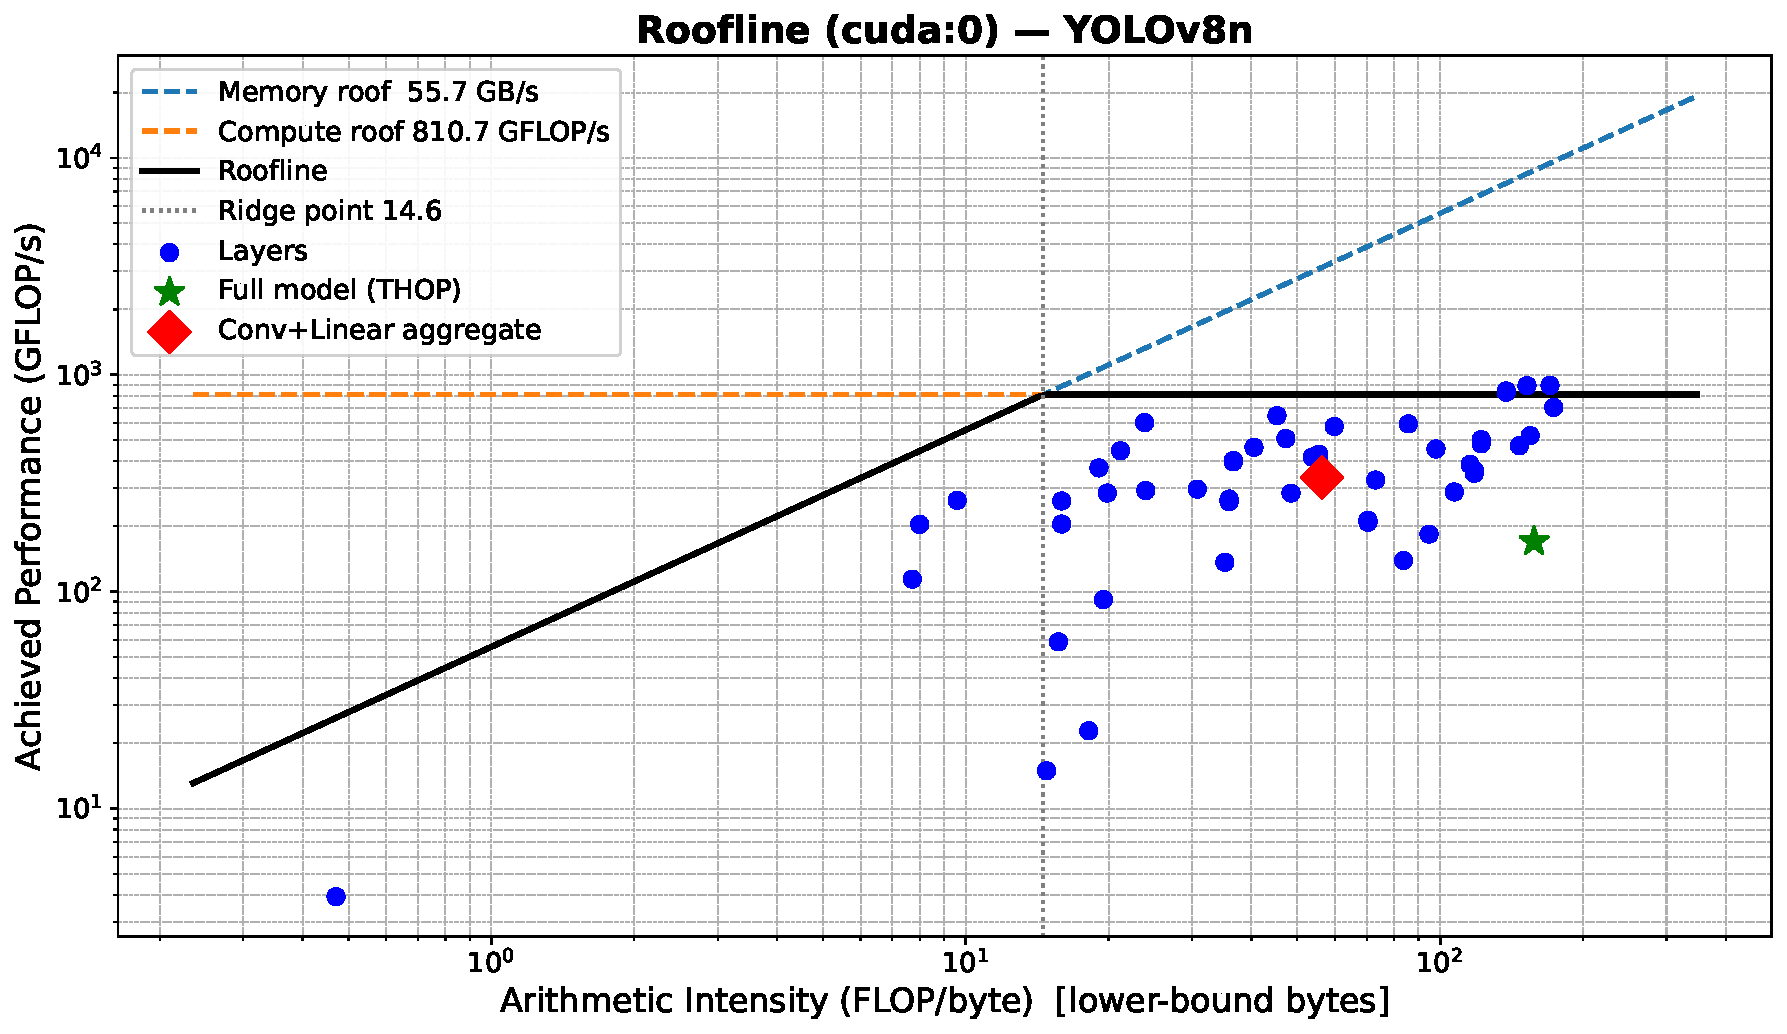
\includegraphics[width=1\linewidth]{pics/roofline_orin_cuda:0_20260402_173102.pdf}
    \caption{Roofline model of YOLOv8n on Jetson Orin Nano (GPU, FP32).}
    \label{fig:roofline_orin}
\end{figure}

Table~\ref{tab:roofline_orin_layers} highlights that, compared to the Raspberry Pi 5,
the majority of convolutional layers on the Orin Nano operate in the compute-bound
regime and achieve substantially higher throughput due to the GPU's much larger
compute capacity and memory bandwidth.

At the same time, the results also show that high per-layer kernel efficiency does
not directly translate into equally high end-to-end model efficiency. Although several
layers approach the measured peak throughput, the overall model reaches only
170.22\,GFLOP/s. This indicates the continued presence of system-level overhead,
including kernel launch overhead, intermediate tensor movement, non-convolutional
operations, and synchronization costs between layers.

Thus, the Orin Nano provides a much more favorable platform for YOLOv8n inference
than the Raspberry Pi 5, but the Roofline analysis still reveals that end-to-end
performance remains constrained by factors beyond raw compute throughput alone.

Detailed per-layer benchmarking results are provided in Appendix~\ref{chap:appendix}.


    %Macbook Pro M3 has declared 150GB/s memory bandwidth ~\cite{apple_memspecs}.


%    \begin{figure}[!h]
%        \centering
%        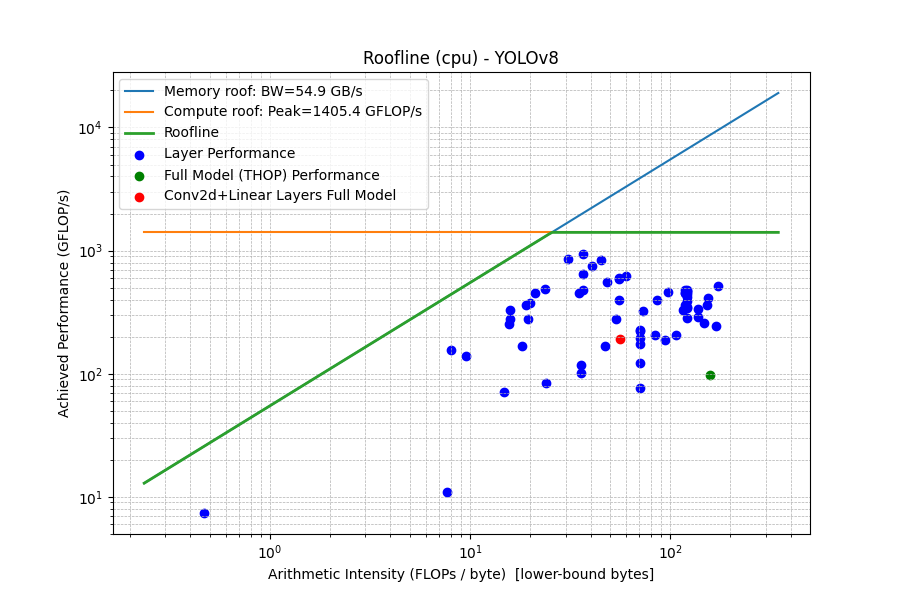
\includegraphics[width=0.8\linewidth]{pics/yolov8n_roofline_cpu_macbook.png}
%        \caption{Roofline model of YOLOv8n on Macbook Pro M3 (CPU, FP32).}
%        \label{fig:roofline_mac_cpu}
%    \end{figure}
%
%    \begin{figure}[!h]
%        \centering
%        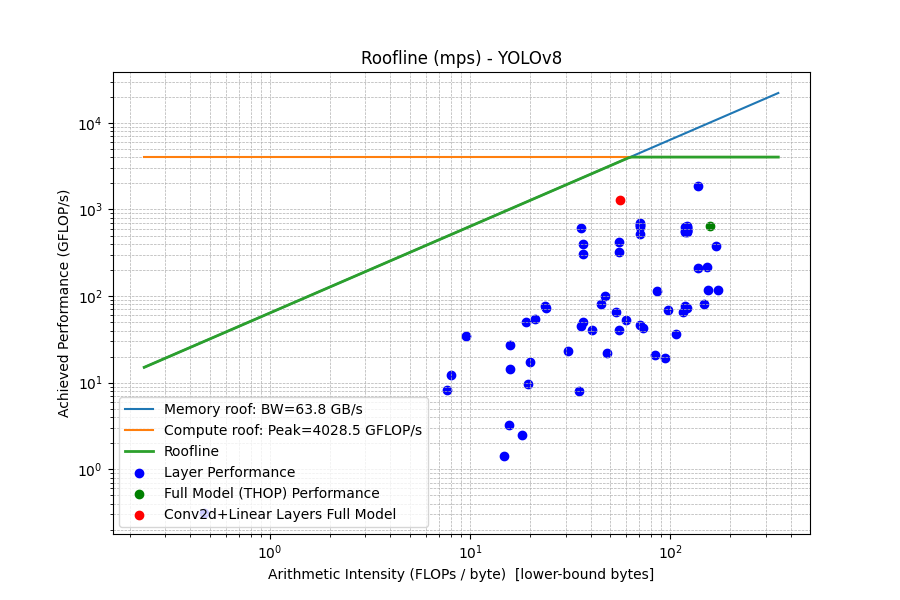
\includegraphics[width=0.8\linewidth]{pics/yolov8n_roofline_mps_macbook.png}
%        \caption{Roofline model of YOLOv8n on Macbook Pro M3 (MPS, FP32).}
%        \label{fig:roofline_mac_mps}
%    \end{figure}

\section{Compiler Performance Comparison}


We evaluated the performance of YOLOv8n models on two hardware platforms: the NVIDIA Orin Nano and the
Raspberry Pi 5. Following this evaluation, we investigated different model compilation approaches tailored
to each target platform.

Due to substantial differences in hardware architectures, the set of available inference frameworks also differs.
Hardware-specific frameworks such as TensorRT are limited to NVIDIA GPUs and therefore cannot be used for a direct
cross-platform comparison. Instead, we assess the performance improvements provided by each framework
relative to a common baseline on the same hardware.

The baseline execution is performed in PyTorch eager mode. In this mode, operations are executed immediately as
Python code is interpreted line by line. The computational graph is constructed dynamically at runtime, which
makes debugging straightforward and enables inspection of intermediate results, such as per-layer performance
metrics presented in the previous section. However, eager execution introduces several limitations: Python-level
overhead for each operation, lack of global graph-level optimization, and limited hardware-specific tuning.
As a result, the model is effectively executed as a sequence of independent operators rather than as an optimized
computational graph.

To address these limitations, the model can be treated as a static graph and optimized using compiler-based
frameworks. A variety of such compilers have been developed to enable hardware-aware optimizations, including
operator fusion, memory planning, and kernel selection. In this section, we evaluate these approaches on the
target hardware platforms.

A standard step in this workflow is converting the model to the ONNX (Open Neural Network Exchange) format.
In this work, we use ONNX export with opset version 17 and enable graph simplification. The opset defines the
set of available operators (e.g., Conv, Add, Resize) and their semantics. Choosing an appropriate opset
version is important: newer opsets may not be fully supported by all backends, while older versions may
lack required operators or optimizations. The opset selection can therefore impact operator decomposition,
kernel count, memory traffic, and opportunities for fusion.

Graph simplification is applied to reduce computational redundancy and streamline the graph structure.
This includes:
\begin{itemize}
\item
Constant folding: precomputing constant expressions (e.g., $x + (2 \times 3) \rightarrow x + 6$)
\item
Node elimination: removing redundant operations such as identity mappings
\item
Subgraph simplification: collapsing sequences of operations into simpler equivalents when possible
\item
Dead code elimination: removing unused branches of the graph

\end{itemize}


While these transformations simplify the graph, backend-specific compilers (e.g., TensorRT, TVM) may perform
additional, more aggressive optimizations such as kernel fusion and layout transformations.

Once converted, the ONNX model can be executed using a variety of inference frameworks. On CPU-based platforms,
commonly used frameworks include PyTorch (via TorchScript or TorchInductor), ONNX Runtime, and TensorFlow Lite.
These frameworks provide different levels of optimization, ranging from general-purpose execution to lightweight
deployment on resource-constrained devices.

On GPU-based platforms, available options include PyTorch with CUDA execution, ONNX Runtime with GPU or TensorRT
execution providers, and TensorRT as a dedicated compiler and runtime for NVIDIA hardware. TensorRT performs
aggressive graph-level and kernel-level optimizations, such as operator fusion, precision calibration
(e.g., FP16/INT8), and memory layout transformations, making it particularly effective for high-performance
inference on NVIDIA devices.

Another notable framework that supports both CPU and GPU targets is Apache TVM. Unlike runtime-focused frameworks,
TVM operates as a deep learning compiler stack that performs end-to-end optimization, including graph
transformations, operator scheduling, and hardware-specific code generation. This approach provides a
high degree of flexibility and control over low-level execution compared to more API-driven frameworks,
although it typically requires more manual tuning and expertise.

\subsection{TVM MetaSchedule Tuning}

Unlike other evaluated frameworks, TVM requires an explicit tuning stage before deployment: MetaSchedule generates
candidate schedules for each extracted operator task, evaluates them on the target device, and compiles the
best-performing implementations into a final binary.
The following subsections report the tuning outcome for each platform and precision, covering which operators
benefited most and where the main performance limits lie.

\subsection{TVM MetaSchedule Tuning Results on Raspberry Pi~5 - FP32}

TVM MetaSchedule was run on the Raspberry Pi~5 (4-core Cortex-A76, AArch64, 2.4\,GHz) for approximately
6 hours and 15 minutes, evaluating 7\,221 valid schedules across 65 operator tasks extracted from the
YOLOv8n Relax graph.
The tuned model achieved a summed task latency of 173.6\,ms and an end-to-end latency of approximately
185--188\,ms, with the small gap attributable to runtime overhead outside the tuned kernels (input
preparation, NMS postprocessing).
Against the 290.1\,ms PyTorch eager baseline, the end-to-end result of approximately 192\,ms corresponds
to a $1.5\times$ improvement.

FP32 tuning on this platform did not enable tensorisation: no task could be mapped to a dedicated ARM
intrinsic, so all performance gains came from cache-blocking, loop reordering, and LLVM auto-vectorisation.
$1{\times}1$ convolutions in the neck and detection head performed best, reaching above 80\,GFLOPS because
their simpler structure maps naturally to vectorised execution.
Larger $3{\times}3$ convolutions in the mid-network also improved once channel dimensions were wide enough
to sustain cache-resident working sets.

The main bottleneck was the initial stem convolution, which processes a 640$\times$640 spatial input with
only three input channels.
This combination yields very low arithmetic intensity that schedule search cannot fundamentally overcome.
When operator multiplicity is accounted for, repeated $3{\times}3$ convolutions inside C2f blocks contributed
more to total runtime than any individually slow operator, confirming that tuning effort is best directed at
frequently executed kernels rather than the single worst-performing layer.
The overall conclusion is that FP32 TVM tuning is beneficial on the Raspberry Pi~5, but gains are bounded
by the absence of tensorisation; a qualitative improvement requires FP16.

\subsection{TVM MetaSchedule Tuning Results on the Jetson Orin Nano GPU - FP32}

On the Jetson Orin Nano GPU, MetaSchedule explored 7\,257 valid schedules across the same 65 operator tasks.
The tuned model achieved a summed task latency of 22\,920\,$\mu$s and an end-to-end latency of 23.38\,ms,
with tuned kernels accounting for almost all of the observed runtime.
Compared with the Raspberry Pi~5 CPU result, this corresponds to a \(7.6\times\) kernel-level speedup,
confirming the expected advantage of GPU execution for convolution-dominated inference.

As in the FP32 CPU case, no task could be tensorised: the GPU benefited from CUDA-specific schedule
parameters (thread-block structure, tiling, memory movement patterns) rather than from Tensor Core mapping.
Unlike the CPU, where $1{\times}1$ convolutions were most efficient, the GPU performed best on large
mid-network $3{\times}3$ convolutions with high channel counts: the best-performing task reached
585.6\,GFLOPS, and several others exceeded 500\,GFLOPS, because the larger working sets gave the GPU
enough parallel work to amortise memory movement.

The stem layer and early low-channel convolutions remained the weakest operators for the same structural
reason as on the CPU: three input channels over a large spatial resolution limits arithmetic intensity.
When multiplicity is taken into account, task~50 (\path{conv2d24}) and task~16 (\path{conv2d11}, appearing
seven times in the graph) were the dominant weighted bottlenecks.
The final end-to-end result of 23.38\,ms was only a modest improvement over the PyTorch eager baseline
(25.12\,ms), and TensorRT remained substantially faster at 11.38\,ms.
This confirms that FP32 GPU tuning without tensorisation leaves significant performance on the table.

\subsection{Raspberry Pi~5 Benchmark Overview - FP32}

All Raspberry Pi~5 experiments were conducted on a Linux system based on the
\path{6.12.62+rpt-rpi-2712} kernel using the AArch64 architecture. The CPU
frequency governor was fixed to \path{performance}, and the CPU was configured
to 2.4\,GHz during the measurements. To reduce thermal and scheduling-related
variation, the benchmarking procedure included a cooldown phase before each
repetition and checks for frequency throttling. Each backend was evaluated over
five repeated runs, with 200 timed inferences per repetition after 30 warm-up
iterations. In addition, each repetition was executed in a fresh subprocess in
order to reduce cross-framework interference, such as cache contamination or
residual runtime state. The comparison was performed using all four available
CPU cores on the Raspberry Pi~5 in order to reflect the maximum CPU throughput
available in this deployment setting. This setup was chosen to reduce
short-term variance and to provide a stable estimate of sustained inference
performance under controlled CPU conditions.

\begin{figure}[t]
    \centering
    \includegraphics[width=\textwidth]{pics/benchmarks/pi5_fp32/pi5_yolov8n_cpu_results_dark_sunset.pdf}
    \caption{YOLOv8n inference performance and power consumption on the Raspberry Pi 5 CPU across the
    evaluated FP32 backends.
    Subfigure~(a) shows the mean end-to-end inference latency with 95\% confidence interval error bars.
    Subfigure~(b) reports mean board power consumption, with error bars indicating standard deviation.
    Subfigure~(c) summarizes the latency--power trade-off, where lower latency and lower power are
    preferable.
    Subfigure~(d) shows energy efficiency in terms of throughput per watt.
    LiteRT achieves the lowest latency and the highest energy efficiency, while TVM and ONNX Runtime
    exhibit similar latency but substantially higher power consumption.}
    \label{fig:pi5_yolov8n_cpu_results}
\end{figure}

The evaluated CPU backends were TVM, ONNX Runtime, TorchCompile, Google AI Edge
LiteRT, and PyTorch eager mode used as a baseline. ONNX Runtime was evaluated
with the \path{CPUExecutionProvider}. Table~\ref{tab:pi5_backend_benchmark}
summarises the measured latency and throughput, while
Table~\ref{tab:pi5_backend_power} summarises power results. These measurements
are further visualised in Figure~\ref{fig:pi5_yolov8n_cpu_results}, which compares
latency, power consumption, the latency--power trade-off, and throughput per watt
across the evaluated CPU backends.

\begin{table}[ht]
\centering
\caption{End-to-end YOLOv8n inference performance on Raspberry Pi~5 CPU.
Values are reported as mean latency $\pm$ half-width of the 95\,\% confidence
interval across 5 isolated repetitions, with 200 timed runs per repetition
after 30 warm-up iterations.}
\label{tab:pi5_backend_benchmark}
\begin{tabular}{lrrr}
\toprule
Backend & Latency (ms) & FPS mean & Median (ms) \\
\midrule
TVM             & $192.0 \pm 7.5$ & 5.21 & 188.8 \\
ONNX Runtime    & $189.2 \pm 7.0$ & 5.28 & 187.2 \\
TorchCompile    & $202.9 \pm 8.5$ & 4.93 & 202.2 \\
LiteRT          & $154.1 \pm 2.5$ & 6.49 & 155.2 \\
PyTorch eager   & $290.1 \pm 2.3$ & 3.45 & 289.8 \\
\bottomrule
\end{tabular}
\end{table}

\paragraph{Overall Performance.}
Among all evaluated frameworks, LiteRT achieved the best overall latency on the
Raspberry Pi~5, with a mean inference time of 154.1\,ms and a throughput of
6.49\,FPS. ONNX Runtime and TVM formed the next performance group, with mean
latencies of 189.2\,ms and 192.0\,ms respectively. TorchCompile was slower than
both compiled deployment backends, reaching a mean latency of 202.9\,ms and a
throughput of 4.93\,FPS. PyTorch eager mode remained the slowest configuration,
with a mean latency of 290.1\,ms and a throughput of 3.45\,FPS. The difference
between ONNX Runtime and TVM was only 2.8\,ms, whereas TorchCompile lagged
behind ONNX Runtime by 13.6\,ms and behind TVM by 10.8\,ms.

\begin{table}[ht]
\centering
\caption{Average power consumption during YOLOv8n inference on Raspberry Pi~5 CPU.}
\label{tab:pi5_backend_power}
\begin{tabular}{lrrr}
\toprule
Backend & Mean Power (mW) & Max Power (mW) & Std (mW) \\
\midrule
TVM             & 4096.2 & 4783.1 & 46.1 \\
ONNX Runtime    & 4043.2 & 5415.1 & 172.5 \\
TorchCompile    & 2291.8 & 2742.5 & 63.2 \\
LiteRT          & 2292.8 & 2591.5 & 14.2 \\
PyTorch eager   & 2316.4 & 2759.8 & 30.3 \\
\bottomrule
\end{tabular}
\end{table}

\paragraph{Stability of Measurements.}
The repeated-run statistics show that TVM and ONNX Runtime had comparable
variability, with standard deviations of 6.03\,ms and 5.65\,ms respectively.
TorchCompile showed a similar but slightly higher variability of 6.86\,ms. In
contrast, PyTorch eager mode and LiteRT were more stable, with standard
deviations of 1.84\,ms and 2.05\,ms. LiteRT therefore combined the best average
performance in this benchmark with comparatively consistent execution.

\paragraph{Power Behaviour.}
TVM and ONNX Runtime showed similar average power draw, measuring 4.10\,W and
4.04\,W respectively. In contrast, TorchCompile, LiteRT, and PyTorch eager mode
all operated near 2.3\,W average board power. LiteRT exhibited the lowest
average power consumption at 2.29\,W, although the difference relative to
TorchCompile was very small. This result is notable because LiteRT was both the
fastest backend in this experiment and the one with the lowest measured average
power consumption.

\paragraph{Interpretation of the Results.}
Although TVM did not outperform LiteRT, it remained competitive with ONNX
Runtime and outperformed TorchCompile in this end-to-end benchmark. TVM
achieved slightly lower latency than TorchCompile while relying on a fully
compiler-driven deployment pipeline based on Relax and MetaSchedule tuning. This
suggests that ahead-of-time compilation through a dedicated inference compiler
remains more effective on this workload than applying \path{torch.compile} to
the original PyTorch model on CPU. At the same time, the results also show that
LiteRT provided the most efficient execution path among the tested frameworks on
Raspberry Pi~5 for this FP32 model.

\paragraph{Conclusion.}
The benchmark results show four practical performance tiers on the Raspberry
Pi~5 CPU. LiteRT delivered the best end-to-end result, combining the lowest
latency, the highest throughput, and the lowest average power consumption. ONNX
Runtime and TVM achieved similar performance, with ONNX Runtime being slightly
faster in the measured configuration. TorchCompile improved substantially over
PyTorch eager mode, but remained slower than both ONNX Runtime and TVM.
PyTorch eager mode was the slowest baseline by a large margin.

Relative to the PyTorch eager baseline, TVM achieved a \(1.51\times\) speedup,
corresponding to a 33.8\,\% reduction in mean inference latency. ONNX Runtime
achieved a \(1.53\times\) speedup, corresponding to a 34.8\,\% latency
reduction. TorchCompile achieved a \(1.43\times\) speedup, corresponding to a
30.1\,\% latency reduction. LiteRT provided the largest improvement, reaching a
\(1.88\times\) speedup and a 46.9\,\% reduction in mean latency. Overall, these
results indicate that TVM is capable of producing competitive CPU inference
performance on Raspberry Pi~5, but in this experiment the most efficient
backend was LiteRT rather than TVM.

\subsection{Jetson Orin Nano GPU Benchmark Overview - FP32}

GPU experiments were conducted on the NVIDIA Jetson Orin Nano using the full
YOLOv8n model in FP32 precision with batch size~1. The evaluated backends were
TVM, ONNX Runtime, TensorRT, PyTorch eager mode, and
\path{torch.compile}. As in the CPU experiments, the benchmark procedure used
isolated repetitions in order to reduce interference between backends.
Table~\ref{tab:orin_backend_benchmark} summarises the measured latency and
throughput, while Table~\ref{tab:orin_backend_power} summarises power results.
These measurements are further visualised in Figure~\ref{fig:orin_yolov8n_fp32_results},
which compares latency, power consumption, the latency--power trade-off, and
throughput per watt across the evaluated GPU backends.

\begin{figure}[t]
    \centering
    \includegraphics[width=\textwidth]{pics/benchmarks/orin_fp32/orin_gpu_fp32_yolov8n_results_dark_sunset.pdf}
    \caption{YOLOv8n FP32 inference performance and power consumption on the NVIDIA Jetson Orin Nano GPU.
    Subfigure~(a) shows mean end-to-end inference latency with 95\% confidence interval error bars.
    Subfigure~(b) reports mean board power consumption, with error bars indicating standard deviation.
    Subfigure~(c) summarizes the latency--power trade-off, where lower latency and lower power are preferable.
    Subfigure~(d) shows energy efficiency in terms of throughput per watt.
    TensorRT achieves the lowest latency and the highest energy efficiency among the evaluated FP32 GPU backends,
        while torch.compile is substantially slower despite lower power draw.}
    \label{fig:orin_yolov8n_fp32_results}
\end{figure}

\begin{table}[ht]
\centering
\caption{End-to-end YOLOv8n inference performance on the NVIDIA Jetson Orin Nano GPU.
Values are reported as mean latency $\pm$ half-width of the 95\,\% confidence
interval across 5 isolated repetitions, with 200 timed runs per repetition
after 30 warm-up iterations.}
\label{tab:orin_backend_benchmark}
\begin{tabular}{lrrr}
\toprule
Backend & Latency (ms) & FPS mean & Median (ms) \\
\midrule
TVM             & $23.38 \pm 0.02$ & 42.77 & 23.39 \\
ONNX Runtime    & $23.18 \pm 0.04$ & 43.14 & 23.17 \\
TorchCompile    & $72.34 \pm 0.47$ & 13.82 & 72.26 \\
TensorRT        & $11.38 \pm 0.02$ & 87.87 & 11.39 \\
PyTorch eager   & $25.12 \pm 0.27$ & 39.81 & 25.12 \\
\bottomrule
\end{tabular}
\end{table}

\paragraph{Overall Performance.}
TensorRT achieved by far the best end-to-end latency on the Jetson Orin Nano,
reaching 11.38\,ms, which corresponds to 87.9\,FPS. ONNX Runtime and TVM
formed a second performance group with nearly identical results, at 23.18\,ms
and 23.38\,ms respectively. PyTorch eager mode was slightly slower at
25.12\,ms, while \path{torch.compile} performed substantially worse than all
other GPU backends, reaching 72.34\,ms.

Relative to the PyTorch eager baseline, TVM achieved a \(1.07\times\) speedup,
corresponding to a 6.9\,\% reduction in mean latency. ONNX Runtime achieved a
\(1.08\times\) speedup and a 7.7\,\% latency reduction. TensorRT provided the
largest improvement, reaching a \(2.21\times\) speedup and a 54.7\,\%
reduction in mean latency. In contrast, \path{torch.compile} was slower than
PyTorch eager mode by a factor of \(2.88\times\).

\begin{table}[ht]
\centering
\caption{Average power consumption during YOLOv8n inference on the NVIDIA Jetson
Orin Nano GPU.}
\label{tab:orin_backend_power}
\begin{tabular}{lrrr}
\toprule
Backend & Mean Power (mW) & Max Power (mW) & Std (mW) \\
\midrule
TVM             & 26007.9 & 26781.1 & 88.7 \\
ONNX Runtime    & 26952.4 & 29632.6 & 84.8 \\
TorchCompile    & 18599.2 & 19967.0 & 76.7 \\
TensorRT        & 28405.8 & 30936.2 & 86.4 \\
PyTorch eager   & 25884.4 & 29186.0 & 168.4 \\
\bottomrule
\end{tabular}
\end{table}

\paragraph{Power and Efficiency.}
In absolute power draw, the GPU backends operated within a relatively narrow
range, from 18.6\,W for \path{torch.compile} to 28.4\,W for TensorRT.
However, when throughput is taken into account, TensorRT was also the most
power-efficient backend, achieving 3.10\,FPS/W. This is approximately
1.9 times higher than TVM and ONNX Runtime, which both reached about
1.6\,FPS/W, and about twice the efficiency of PyTorch eager mode. Although
\path{torch.compile} consumed the least power, its very low throughput made
it the least efficient backend overall.

\paragraph{Interpretation of the TVM Result.}
The TVM GPU result is notable for two reasons. First, its end-to-end latency
was essentially identical to ONNX Runtime, with a difference of only 0.20\,ms.
Second, TVM still outperformed PyTorch eager mode, although the margin was much
smaller than on the CPU. This suggests that, on the Orin Nano GPU, the main
convolution-heavy parts of the model are already executed efficiently by mature
CUDA libraries across multiple frameworks, which reduces the practical
advantage of compiler-level scheduling alone. In other words, TVM remained
competitive, but did not establish a clear lead over ONNX Runtime on this
platform.

\paragraph{Conclusion.}
The GPU benchmark results reveal three practical performance tiers. TensorRT
forms the clear top tier, achieving both the lowest latency and the highest
power efficiency. ONNX Runtime and TVM form a second tier with nearly identical
performance, while PyTorch eager mode is only slightly slower. In contrast,
\path{torch.compile} was not competitive for this workload in the tested
configuration. Overall, these results show that TensorRT was the most effective
deployment backend for YOLOv8n on the Jetson Orin Nano GPU, whereas TVM and
ONNX Runtime delivered similar and competitive FP32 performance.

Relative to the PyTorch eager baseline, TVM achieved a \(1.07\times\) speedup,
equivalent to a 6.9\,\% reduction in mean inference latency, and ONNX Runtime
achieved a \(1.08\times\) speedup with a 7.7\,\% latency reduction. TensorRT
provided the largest improvement, reaching a \(2.21\times\) speedup and a
54.7\,\% reduction in mean latency. In contrast, \path{torch.compile} failed
to improve upon the baseline and instead increased latency by a factor of
\(2.88\times\). These results indicate that TVM can provide competitive GPU
inference performance on the Jetson Orin Nano, but in this experiment the
largest practical advantage was obtained with TensorRT.

\section{FP16 Inference Results}

Before discussing the measured FP16 results, it is important to clarify that conversion to FP16 is not
the same as quantization. In FP16 inference, weights and activations remain in floating-point representation,
but with reduced numerical precision compared to FP32. By contrast, quantization usually refers
to mapping tensors into lower-bit integer or fixed-point formats, such as INT8,
which changes not only the storage format but also the arithmetic model used
during execution. FP16 should therefore be understood as reduced-precision
floating-point inference rather than true quantization.

This distinction is important for interpreting the following measurements. Reducing precision from FP32 to FP16 can
decrease memory traffic and improve throughput on hardware with native half-precision support, often with only a
small impact on model accuracy. However, the resulting performance behaviour is different from that of integer
quantization, since the model still operates in a floating-point domain.
The following subsection therefore evaluates FP16 as a  separate optimisation path and analyses
its effect on latency, throughput, and overall deployment efficiency.

\subsection{TVM MetaSchedule Tuning Results on the Jetson Orin Nano GPU - FP16}

TVM MetaSchedule was re-run on the Jetson Orin Nano GPU using a FP16 version of the YOLOv8n graph,
converted from the FP32 ONNX export using \path{onnxconverter-common} with \path{keep\_io\_types=False}.
The tuning campaign ran for approximately 18 hours and explored 6\,477 valid schedules across 66 operator
tasks.
The tuned model achieved a summed task latency of 9\,872\,$\mu$s and an end-to-end latency of 12.45\,ms,
corresponding to a \(2.3\times\) kernel-level improvement and a \(1.88\times\) end-to-end speedup over the
FP32 result.

The critical difference from FP32 was that FP16 enabled tensorised execution via Warp Matrix Multiply-Accumulate (WMMA)
on the Orin Nano GPU.
In FP32, no task could be mapped to a hardware intrinsic and all schedules used standard CUDA thread-block
tiling.
In FP16, a large fraction of convolutional tasks were tensorised, raising peak operator throughput from
585.6\,GFLOPS to 1\,872.7\,GFLOPS -- a \(3.2\times\) gain in peak kernel efficiency.
The speedup therefore arose not only from halved data movement but from a qualitatively different
optimisation path: MetaSchedule could now search over implementations that directly exploit the GPU's
matrix-multiplication hardware.

The main bottleneck pattern remained unchanged: the stem layer (3 input channels, 640$\times$640 spatial
resolution) could not benefit from tensorisation and remained the least efficient individual operator even
in FP16.
When multiplicity is included, repeated backbone and neck convolutions -- notably task~50 (\path{conv2d24})
and task~16 (\path{conv2d11}) -- again dominated total runtime.
TensorRT remained faster at 6.31\,ms, indicating that vendor-specific optimisations still provide an
additional margin beyond what MetaSchedule found.
Nevertheless, FP16 tuning establishes TVM as a genuinely competitive deployment backend: it cut end-to-end
latency from 23.38\,ms to 12.45\,ms, confirming FP16 as the appropriate precision target for TVM-based deployment
on Orin-class hardware.

\subsection{Jetson Orin Nano GPU Benchmark Overview - FP16}

GPU experiments were also conducted on the NVIDIA Jetson Orin Nano using the
full YOLOv8n model in FP16 precision with batch size~1. The evaluated backends
were TVM, ONNX Runtime, TensorRT, PyTorch eager mode, and
\texttt{torch.compile}. As in the previous benchmark sections, the comparison
was performed using isolated repetitions in order to reduce interference between
frameworks. Table~\ref{tab:orin_fp16_backend_benchmark} summarises the measured
latency and throughput, while Table~\ref{tab:orin_fp16_backend_power}
summarises power results. Figure~\ref{fig:orin_fp32_vs_fp16_results} further
compares the FP16 measurements against the corresponding FP32 results, showing
the latency, FP16 speedup, power consumption, and energy efficiency for each
backend.

\begin{figure}[t]
    \centering
    \includegraphics[width=\textwidth]{pics/benchmarks/fp16_vs_fp32/orin_gpu_fp32_vs_fp16_successful_runs_dark_sunset.pdf}
    \caption{FP32 versus FP16 YOLOv8n inference on the NVIDIA Jetson Orin Nano GPU.
    Subfigure~(a) compares mean end-to-end latency for each backend, with error bars indicating the half-width of
    the 95\% confidence interval.
    Subfigure~(b) reports the FP16 latency speedup relative to FP32 for the same backend, where values above
        $1.0\times$ indicate that FP16 is faster.
    Subfigure~(c) compares mean board power consumption, and Subfigure~(d) compares energy efficiency in terms of
        throughput per watt.
    TensorRT and TVM obtain the strongest FP16 latency improvements, while \texttt{torch.compile} and PyTorch eager
        mode do not benefit from FP16 in this experiment.}
    \label{fig:orin_fp32_vs_fp16_results}
\end{figure}


\begin{table}[ht]
\centering
\caption{End-to-end YOLOv8n inference performance on the NVIDIA Jetson Orin Nano GPU in FP16 precision.
Values are reported as mean latency $\pm$ half-width of the 95\,\% confidence
interval across 5 isolated repetitions, with 200 timed runs per repetition
after 30 warm-up iterations.}
\label{tab:orin_fp16_backend_benchmark}
\begin{tabular}{lrrr}
\toprule
Backend & Latency (ms) & FPS mean & Median (ms) \\
\midrule
TVM             & $12.45 \pm 0.05$ & 80.35 & 12.43 \\
ONNX Runtime    & $16.95 \pm 0.02$ & 59.00 & 16.96 \\
TorchCompile    & $72.72 \pm 0.21$ & 13.75 & 72.76 \\
TensorRT        & $6.31 \pm 0.01$  & 158.55 & 6.31 \\
PyTorch eager   & $27.36 \pm 0.24$ & 36.55 & 27.34 \\
\bottomrule
\end{tabular}
\end{table}

\paragraph{Overall Performance.}
TensorRT achieved the best end-to-end latency in the FP16 setting, reaching
6.31\,ms, which corresponds to 158.6\,FPS. TVM formed the second-best result at
12.45\,ms and substantially outperformed ONNX Runtime, which reached 16.95\,ms.
PyTorch eager mode was considerably slower at 27.36\,ms, while
\path{torch.compile} again performed substantially worse than all other
backends, reaching 72.72\,ms.

Relative to the PyTorch eager baseline, TVM achieved a \(2.20\times\) speedup,
corresponding to a 54.5\,\% reduction in mean latency. ONNX Runtime achieved a
\(1.61\times\) speedup and a 38.1\,\% latency reduction. TensorRT provided the
largest improvement, reaching a \(4.34\times\) speedup and a 76.9\,\%
reduction in mean latency. In contrast, \path{torch.compile} was slower than
PyTorch eager mode by a factor of \(2.66\times\).

\begin{table}[ht]
\centering
\caption{Average power consumption during YOLOv8n inference on the NVIDIA Jetson
Orin Nano GPU in FP16 precision.}
\label{tab:orin_fp16_backend_power}
\begin{tabular}{lrrr}
\toprule
Backend & Mean Power (mW) & Max Power (mW) & Std (mW) \\
\midrule
TVM             & 21770.0 & 24514.2 & 122.6 \\
ONNX Runtime    & 24601.7 & 29104.0 & 88.3 \\
TorchCompile    & 16760.5 & 17874.5 & 33.9 \\
TensorRT        & 24342.7 & 26500.5 & 19.0 \\
PyTorch eager   & 20282.6 & 20852.0 & 79.9 \\
\bottomrule
\end{tabular}
\end{table}

\paragraph{Power and Efficiency.}
In absolute power draw, the FP16 GPU backends again operated within a
relatively narrow range, from 16.8\,W for \path{torch.compile} to 24.6\,W for
ONNX Runtime. However, throughput differed much more strongly than power, which
made efficiency comparisons especially informative. TensorRT achieved the best
efficiency at approximately 6.51\,FPS/W, followed by TVM at about 3.69\,FPS/W.
PyTorch eager mode reached about 1.80\,FPS/W, and ONNX Runtime about
2.40\,FPS/W. Although \path{torch.compile} consumed the least power, its low
throughput again made it the least competitive backend in practice.

\paragraph{Interpretation of the TVM Result.}
The TVM FP16 result is particularly notable because, unlike in FP32, TVM no
longer merely matched ONNX Runtime but clearly outperformed it. Its latency was
4.50\,ms lower than ONNX Runtime, corresponding to an additional reduction of
approximately 26.6\,\%. This indicates that FP16 compilation gave TVM access to
optimisation opportunities that were not available in the FP32 case, most
importantly tensorised execution for a large fraction of the convolutional
operators. As a result, TVM moved from being merely competitive in FP32 to
becoming the second-best backend overall in FP16.

At the same time, TensorRT still remained significantly faster, with a latency
of 6.31\,ms compared with 12.45\,ms for TVM. This shows that even though TVM
benefited greatly from FP16 compilation, additional backend-specific
optimisations still remain available beyond what MetaSchedule found in this
work.

\paragraph{Conclusion.}
The FP16 benchmark results reveal a clearer separation between deployment
backends than in the FP32 GPU case. TensorRT formed the top tier with the best
latency, throughput, and efficiency. TVM formed a strong second tier and
substantially outperformed ONNX Runtime, PyTorch eager mode, and
\path{torch.compile}. ONNX Runtime remained competitive but was noticeably
slower than TVM, while PyTorch eager mode was substantially slower than all
three specialised deployment paths. As in the FP32 case, \path{torch.compile}
was not competitive for this workload in the tested configuration.

Overall, these results indicate that FP16 is the most favourable precision
setting for TVM deployment on the Jetson Orin Nano GPU. In this configuration,
TVM no longer merely matched other general deployment runtimes, but delivered a
clear practical advantage over ONNX Runtime and PyTorch eager mode. However,
TensorRT still provided the fastest overall execution and remained the most
effective deployment backend in the final comparison.

\subsection{FP16 Inference on the Raspberry Pi~5 CPU}

To investigate whether half-precision arithmetic provides a runtime benefit on
the Raspberry Pi~5, the YOLOv8n model was re-evaluated at FP16 precision across
all applicable backends. The FP16 ONNX model was generated from the FP32 export
using \path{onnxconverter-common} with \path{keep\_io\_types=False}, producing
a graph in which all weights, activations, and the input tensor are represented
as 16-bit floats. TVM was re-tuned on this model, yielding a separately compiled
\path{.so} library. All other backends received the same FP16 ONNX as input.

\paragraph{TVM FP16 Tuning Session.}
For TVM, the FP16 tuning campaign covered 65 operator tasks in approximately 4 hours and 6 minutes,
compared with 6 hours and 15 minutes for FP32.
The shorter run reflects the stronger latency signal from FP16 kernels: once LLVM finds a schedule that
packs eight \path{float16} values into a 128-bit NEON (ARM Advanced SIMD extension) register rather than
four \path{float32} values, the improvement is immediately visible and the tuner shifts to refinement
instead of exploration.
As in FP32, no task could be tensorised -- the three-dimensional convolution reduction (input channels,
kernel height, kernel width) cannot be mapped to NEON's one-dimensional dot-product intrinsic -- so all
schedules relied on cache-blocked tiling with \path{float16x8} auto-vectorisation.
Peak operator throughput rose from 87.1\,GFLOPS (FP32) to 169.2\,GFLOPS (FP16), a \(1.94\times\) ratio
consistent with the theoretical $2\times$ gain from halving element width within a fixed 128-bit register.

\paragraph{End-to-End Benchmark Results.}
Figure~\ref{fig:pi5_fp32_vs_fp16_results} visualises the successful FP16 runs
against their corresponding FP32 measurements on the Raspberry Pi~5 CPU,
including latency, FP16 speedup, power consumption, and energy efficiency.
Table~\ref{tab:pi5_fp32_fp16} presents the full benchmark comparison between
FP32 and FP16 precision across all backends on the Raspberry Pi~5, including
the unsuccessful or fallback FP16 cases.

\begin{figure}[t]
    \centering
    \includegraphics[width=\textwidth]{pics/benchmarks/fp16_vs_fp32/pi5_cpu_fp32_vs_fp16_successful_runs_dark_sunset.pdf}
    \caption{FP32 versus FP16 YOLOv8n inference on the Raspberry Pi~5 CPU for backends with successful FP16 runs.
    Subfigure~(a) compares mean end-to-end latency, with error bars indicating the half-width of the 95\% confidence
    interval where available.
    Subfigure~(b) reports the FP16 latency speedup relative to FP32 for the same backend, where values above
        $1.0\times$ indicate that FP16 is faster.
    Subfigure~(c) compares mean board power consumption, and Subfigure~(d) compares energy efficiency in terms of
        throughput per watt.
    TVM is the only backend that shows a clear FP16 latency improvement on the Raspberry Pi~5 CPU, while TFLite
        remains nearly unchanged and TorchCompile becomes substantially slower.}
    \label{fig:pi5_fp32_vs_fp16_results}
\end{figure}

\begin{table}[ht]
\centering
\caption{FP32 vs FP16 inference on the Raspberry Pi~5 CPU
         (5 repetitions $\times$ 200 runs, 30 warm-up runs,
         performance governor, batch size~1, 640$\times$640 input).
         ORT and PyTorch FP16 results are estimated from single-repetition
         measurements; TorchCompile FP16 is from the rigorous run.}
\label{tab:pi5_fp32_fp16}
\begin{tabular}{lrrrr}
\toprule
Backend & FP32 mean (ms) & FP16 mean (ms) & Ratio & FP16 status \\
\midrule
TVM          & 192.01 & 122.44 & $1.57\times$ faster & real fp16 \\
ONNXRuntime  & 189.23 & $>$900\,s & timeout           & no fp16 Conv \\
TFLite       & 154.06 & 153.27 & $1.00\times$         & weights only \\
TorchCompile & 200.39 & 983.08 & $4.9\times$ slower   & GEMM fallback \\
PyTorch      & 290.13 & $\approx$11\,000 & $38\times$ slower & scalar loop \\
\bottomrule
\end{tabular}
\end{table}

\paragraph{TVM - the Only Backend with Real FP16 Acceleration.}
TVM reduced its end-to-end latency from 192.01\,ms to 122.44\,ms, a speedup
of $1.57\times$. This improvement stems from a qualitative change in the
generated code: LLVM emits \path{VFMA.F16} NEON instructions that operate on
eight \path{float16} values in parallel within the same 128-bit register that
previously held four \path{float32} values. The gap between the measured
$1.57\times$ end-to-end speedup and the theoretical $2\times$ kernel-level
ceiling is explained by two factors. First, non-arithmetic operators - splits,
concatenations, and the upsampling layers of the FPN neck - execute at the
same speed regardless of element width. Second, the initial stem convolution,
which has only three input channels, cannot fill the eight available FP16 NEON
lanes; its latency therefore improves only marginally between precisions.
Both of these effects are irreducible at the schedule level and represent
genuine architectural constraints of the YOLOv8n graph on a scalar-SIMD
processor.

\paragraph{ONNXRuntime - Timeout Due to Missing FP16 Convolution Kernel.}
The ONNXRuntime worker exceeded the 900-second subprocess timeout and produced
no result. This is not a measurement artefact but a direct consequence of the
MLAS math library not implementing a half-precision convolution kernel for ARM.
When MLAS encounters a FP16 \path{Conv} operator, it inserts
\path{Cast(float16$\to$float32)} nodes before and after every convolution and
computes the operation in FP32. The resulting per-inference latency is estimated
at approximately 7\,100\,ms - derived by scaling the FP32 ORT result by the
same regression factor observed in PyTorch eager FP16. With 30 warm-up and 200
timed iterations, the total subprocess time would reach approximately
1\,630\,seconds, well above the timeout. This behaviour has been documented in
the ONNX Runtime issue tracker
and reflects a fundamental gap in MLAS coverage rather than a configuration
error.

\paragraph{TFLite - Storage Benefit Only.}
TFLite produced virtually identical latency at both precisions: 154.06\,ms in
FP32 and 153.27\,ms in FP16, a difference smaller than one standard deviation.
This result confirms that TFLite's FP16 model format stores weights as 16-bit
values but promotes all arithmetic to FP32 before computation on this platform.
The model occupies half the memory, which can reduce cache pressure and improve
load time, but no arithmetic throughput benefit accrues at inference time. The
near-identical power consumption at both precisions (2\,293\,mW FP16 vs
2\,293\,mW FP32) corroborates this interpretation.

\paragraph{TorchCompile and PyTorch - Regression Under FP16.}
Both PyTorch-based backends degraded significantly at FP16. PyTorch eager mode
regressed by a factor of $38\times$, from 290\,ms to approximately 11\,000\,ms.
When \path{model.half()} is called on a CPU device, the ATen kernel dispatcher
finds no half-precision GEMM implementation and falls back to an element-wise
scalar loop that processes each \path{float16} value individually, upcasting
to \path{float32} for each multiply-accumulate step.

TorchCompile degraded by $4.9\times$, from 200\,ms to 983\,ms. This is less
severe than PyTorch eager because the Inductor backend successfully generates
vectorised C++ code for element-wise operations such as the SiLU activation and
residual additions. However, the convolution operators - which dominate total
runtime - are not covered by Inductor's FP16 CPU code generation path and still
fall through to the same ATen scalar fallback. The resulting graph alternates
between fast Inductor-compiled segments and slow ATen scalar segments, with
type-conversion overhead at every boundary. The net effect is that TorchCompile
FP16 is slower than TorchCompile FP32 despite Inductor genuinely improving some
of the individual operations.

\paragraph{Power Consumption.}
Table~\ref{tab:pi5_fp16_power} reports the mean board power measured during
inference for the backends that completed successfully.

\begin{table}[ht]
\centering
\caption{Power and energy-efficiency comparison on the Raspberry Pi~5 CPU
         at FP16 precision (successful runs only).}
\label{tab:pi5_fp16_power}
\begin{tabular}{lrrrr}
\toprule
Backend & Mean latency (ms) & Power (mW) & Energy/frame (mJ) & FPS/W \\
\midrule
TVM          & 122.44 & 4\,232 & 517.7 & 1.93 \\
TFLite       & 153.27 & 2\,291 & 351.1 & 2.85 \\
TorchCompile & 983.08 & 2\,202 & 2\,164.0 & 0.45 \\
\bottomrule
\end{tabular}
\end{table}

TFLite achieves the best energy efficiency at FP16 (2.85\,FPS/W), primarily
because its lightweight runtime draws substantially less board power than the
TVM or Inductor runtimes while delivering competitive latency. TVM draws more
power (4\,232\,mW) due to higher CPU utilisation from its densely vectorised
kernels, but still outperforms TFLite in absolute latency. TorchCompile consumes
the least power per unit time but has by far the highest energy per frame
because of its poor throughput.

\paragraph{Overall Assessment.}
The Raspberry Pi~5 FP16 results demonstrate that half-precision acceleration
on ARM CPU is a compiler problem rather than a hardware problem. The Cortex-A76
implements ARMv8.2-A FEAT\_FP16, providing native \path{float16} arithmetic
in its NEON units. The bottleneck is that no major CPU runtime library - MLAS,
OpenBLAS, or the ATen dispatcher - implements a half-precision GEMM kernel for
this target. Only TVM, which generates the convolution kernel directly as LLVM
IR and lets the AArch64 backend select \path{float16x8} NEON instructions,
can exploit the available hardware capability. The result is a $1.57\times$
end-to-end speedup over FP32 TVM, achieved within a four-hour tuning session.
All other frameworks either time out, regress, or show no improvement at
FP16 precision. This finding has a direct practical implication: deploying
FP16 models on edge CPU platforms without a compilation-based inference
engine yields no latency benefit and may cause severe degradation.

\section{Accuracy Comparison Across Inference Frameworks}
\label{sec:accuracy_comparison_frameworks}

To verify that different inference frameworks preserve the predictive quality of the original model, YOLOv8n was
evaluated across several backends and compared against the default PyTorch eager FP32 implementation. Since large
multi-backend evaluation is memory-intensive, especially when repeatedly loading different runtimes and exported
artifacts, the comparison was performed on a 1000-image subset of the validation set rather than on the full
validation split. Although smaller than the full COCO validation set, this subset is sufficient to determine whether
export, compilation, or reduced precision introduce any meaningful degradation in detection quality.

All backends were evaluated using the same basic setup: image size $640 \times 640$, batch size $1$, confidence
threshold $0.001$, IoU threshold $0.7$, and maximum number of detections $300$. Each backend was loaded and evaluated
sequentially in isolation in order to reduce memory pressure and avoid interference between runtime environments.

Because the GPU-oriented and CPU-oriented backends were evaluated in separate comparison runs, they are presented
separately below. The small difference between the corresponding PyTorch FP32 baseline values should therefore be
interpreted as run-to-run variation rather than as a framework effect.

\subsubsection{GPU-Oriented Backends}

The GPU-side comparison included PyTorch eager FP32/FP16, ONNX Runtime CUDA FP32/FP16, TensorRT FP32/FP16, and
TVM GPU FP32/FP16. Absolute results are shown in Table~\ref{tab:acc_abs_gpu_backends}, and relative changes with
respect to the PyTorch eager FP32 baseline of the same run are given in Table~\ref{tab:acc_rel_gpu_backends}.

\begin{table}[ht]
\centering
\caption{Absolute detection metrics for GPU-oriented backends on 1000 validation images.}
\label{tab:acc_abs_gpu_backends}
\begin{tabular}{lcccc}
\toprule
Backend & Precision & Recall & mAP50 & mAP50--95 \\
\midrule
PyTorch eager FP32     & 0.6299 & 0.4878 & 0.5384 & 0.3899 \\
PyTorch eager FP16     & 0.6301 & 0.4880 & 0.5385 & 0.3898 \\
ONNX Runtime FP32      & 0.6283 & 0.4905 & 0.5386 & 0.3899 \\
ONNX Runtime FP16      & 0.6300 & 0.4888 & 0.5387 & 0.3900 \\
TensorRT FP32          & 0.6282 & 0.4893 & 0.5385 & 0.3899 \\
TensorRT FP16          & 0.6248 & 0.4907 & 0.5385 & 0.3901 \\
TVM GPU FP32           & 0.6319 & 0.4889 & 0.5390 & 0.3899 \\
TVM GPU FP16           & 0.6290 & 0.4893 & 0.5381 & 0.3894 \\
\bottomrule
\end{tabular}
\end{table}

\begin{table}[ht]
\centering
\caption{Relative changes (\%) for GPU-oriented backends with respect to PyTorch eager FP32.}
\label{tab:acc_rel_gpu_backends}
\begin{tabular}{lcccc}
\toprule
Backend & $\Delta$ Precision (\%) & $\Delta$ Recall (\%) & $\Delta$ mAP50 (\%) & $\Delta$ mAP50--95 (\%) \\
\midrule
PyTorch eager FP16     & +0.03 & +0.03 & +0.02 & -0.01 \\
ONNX Runtime FP32 & -0.25 & +0.54 & +0.05 & +0.02 \\
ONNX Runtime FP16 & +0.02 & +0.19 & +0.06 & +0.02 \\
TensorRT FP32          & -0.27 & +0.30 & +0.02 & +0.01 \\
TensorRT FP16          & -0.81 & +0.58 & +0.03 & +0.07 \\
TVM GPU FP32           & +0.32 & +0.23 & +0.12 & +0.00 \\
TVM GPU FP16           & -0.14 & +0.29 & -0.05 & -0.12 \\
\bottomrule
\end{tabular}
\end{table}

The GPU results show that all backends preserved accuracy very well. The observed changes in mAP50 and mAP50--95 were
very small, indicating that export to ONNX Runtime, TensorRT, and TVM did not introduce any practically meaningful
loss in detector quality. FP16 also remained stable overall. PyTorch FP16, ONNX Runtime CUDA FP16, and TensorRT FP16
all stayed extremely close to the FP32 baseline. TVM GPU FP16 showed the largest negative deviation on the GPU side,
but the absolute change remained small.

\subsubsection{CPU-Oriented Backends}

A separate CPU-side comparison included PyTorch eager FP32/FP16, ONNX Runtime CPU, TFLite CPU FP32/FP16, and
TVM CPU FP32/FP16. Absolute results are shown in Table~\ref{tab:acc_abs_cpu_backends}, and relative changes with
respect to the PyTorch eager FP32 baseline of that run are shown in Table~\ref{tab:acc_rel_cpu_backends}.

\begin{table}[ht]
\centering
\caption{Absolute detection metrics for CPU-oriented backends on 1000 validation images.}
\label{tab:acc_abs_cpu_backends}
\begin{tabular}{lcccc}
\toprule
Backend & Precision & Recall & mAP50 & mAP50--95 \\
\midrule
PyTorch eager FP32  & 0.6291 & 0.4884 & 0.5384 & 0.3898 \\
PyTorch eager FP16  & 0.6291 & 0.4884 & 0.5384 & 0.3898 \\
ONNX Runtime CPU    & 0.6291 & 0.4884 & 0.5384 & 0.3898 \\
TFLite FP32 CPU     & 0.6291 & 0.4884 & 0.5384 & 0.3898 \\
TFLite FP16 CPU     & 0.6276 & 0.4905 & 0.5384 & 0.3899 \\
TVM CPU FP32        & 0.6291 & 0.4884 & 0.5384 & 0.3898 \\
TVM CPU FP16        & 0.6280 & 0.4894 & 0.5395 & 0.3900 \\
\bottomrule
\end{tabular}
\end{table}

\begin{table}[ht]
\centering
\caption{Relative changes (\%) for CPU-oriented backends with respect to PyTorch eager FP32.}
\label{tab:acc_rel_cpu_backends}
\begin{tabular}{lcccc}
\toprule
Backend & $\Delta$ Precision (\%) & $\Delta$ Recall (\%) & $\Delta$ mAP50 (\%) & $\Delta$ mAP50--95 (\%) \\
\midrule
PyTorch eager FP16 & +0.00 & +0.00 & +0.00 & +0.00 \\
ONNX Runtime CPU   & -0.00 & +0.00 & +0.00 & +0.00 \\
TFLite FP32 CPU    & -0.00 & -0.00 & +0.00 & +0.00 \\
TFLite FP16 CPU    & -0.24 & +0.43 & +0.00 & +0.03 \\
TVM CPU FP32       & -0.00 & -0.00 & +0.00 & +0.00 \\
TVM CPU FP16       & -0.17 & +0.20 & +0.20 & +0.06 \\
\bottomrule
\end{tabular}
\end{table}

The CPU results are similarly stable. PyTorch FP16, ONNX Runtime CPU, TFLite FP32 CPU, and TVM CPU FP32 reproduced
the PyTorch FP32 baseline almost exactly. TFLite FP16 and TVM CPU FP16 introduced small shifts in the balance
between precision and recall, but the aggregate mAP values remained effectively unchanged. In particular,
TVM CPU FP16 slightly improved mAP50 and mAP50--95 while slightly reducing precision, again indicating only minor
numerical variation rather than a meaningful change in model behavior.

\subsubsection{Discussion}

Across both GPU and CPU experiments, no framework caused a significant drop in detection quality. The most important
result is that mAP50 and especially mAP50--95 remained very close to the corresponding PyTorch eager FP32 baselines
in all runs. This shows that the predictive behavior of YOLOv8n is preserved well across
the evaluated deployment frameworks.

Because all backends execute the same trained model, the remaining small differences should not be interpreted
as one framework being inherently more accurate than another. Instead, they are better explained by runtime-dependent
numerical variation. Different inference frameworks may use different kernel implementations, operator fusion patterns,
accumulation orders, and precision conversion paths. In object detection, even tiny numerical differences can slightly
shift confidence scores or bounding box coordinates, which may then change whether a detection is kept or removed
during thresholding and non-maximum suppression. This explains the recurring pattern that some FP16 configurations
slightly reduce precision while slightly increasing recall, without materially changing the overall mAP.

Overall, these results indicate that framework conversion and mixed-precision inference do not meaningfully
degrade YOLOv8n accuracy in the evaluated setups. This justifies focusing the later comparison primarily on latency,
throughput, and hardware efficiency, since accuracy was effectively preserved across both GPU-oriented and
CPU-oriented backends.


\section{Influence of Quantization on YOLOv8n}
\label{sec:quantization_yolov8n}

Quantization is often presented as a direct way to improve inference efficiency by reducing numerical precision,
model size, and memory bandwidth requirements. In practice, however, quantization remains a difficult deployment
problem. Its final effect depends not only on the quantization method itself, but also on the maturity of the
compiler or runtime stack, the target hardware, and the way quantized operators are represented in the exported
graph.

\subsection{INT8 Inference on NVIDIA Orin Nano GPU}
\label{sec:orin_int8_results}

For this reason, the quantization study in this thesis focuses on practical deployment behavior rather than on
theoretical INT8 speedup alone. The experiments were carried out on the Jetson Orin Nano GPU and compared FP32 and
INT8 inference across several deployment paths. The PyTorch FP32 model served as the reference baseline. ONNX Runtime
was evaluated using statically quantized QuantizeLinear--DequantizeLinear (QDQ) graphs, while TensorRT was evaluated both with an implicit INT8
calibration path starting from an FP32 ONNX model and with a QDQ-based INT8 ONNX graph.

A first important observation is that efficient quantization support is not uniformly available across deployment
frameworks. For example, while Apache TVM provides strong support for FP32 compilation and scheduling through
MetaSchedule, the Relax-based quantization flow remains immature in the tested version. In practice, implementing a
custom INT8 path would require calibration tooling, graph rewriting, requantization logic, and validated low-precision
kernels, which is beyond the scope of the present thesis. By contrast, ONNX Runtime and TensorRT both provide
deployable INT8 paths, but their practical outcomes differ substantially.

ONNX Runtime static quantization inserts explicit \path{QuantizeLinear} and \path{DequantizeLinear} operators into
the computational graph. Although this representation is portable, it may also introduce substantial overhead when
these conversions are not fully fused away by the execution backend. In a convolution-heavy architecture such as
YOLOv8n, this is especially problematic, since quantization boundaries may appear repeatedly throughout the network.
TensorRT can ingest such QDQ graphs, but the resulting execution still contains additional quantization-related
transformations, reformatting steps, and copy operations. An alternative TensorRT path is implicit INT8 calibration,
where the engine is built from an FP32 ONNX model and calibrated directly for TensorRT's internal low-precision
execution. This remains one of the most accessible hardware-native INT8 deployment mechanisms on Jetson-class devices.

Table~\ref{tab:int8_accuracy_comparison} summarizes the detection accuracy results. All measurements were performed on
the same set of 1000 images from the COCO validation split. TensorRT FP32 reproduces the PyTorch FP32 baseline almost
exactly, confirming that TensorRT export by itself does not meaningfully affect model quality. In contrast, all
evaluated INT8 paths reduce accuracy, but the magnitude of the degradation varies strongly. The ONNX Runtime QDQ
models lead to a moderate drop of approximately 6--9\% in mAP, depending on the calibration subset. TensorRT implicit
INT8 calibration performs worse in accuracy than the FP32 TensorRT engine and also remains less accurate than the
previously evaluated FP16 TensorRT configuration, but it is still clearly more accurate than the TensorRT QDQ path.

The TensorRT QDQ engine exhibits the largest accuracy degradation, with mAP50 decreasing by more than 25\% and
mAP50--95 by nearly 42\%, which makes this variant impractical for deployment in the tested setup. A likely reason is
that the ONNX QDQ graph requires additional adjustment before efficient TensorRT execution becomes possible. In
particular, TensorRT does not support the default UINT8 zero-point convention commonly used in ONNX graphs, while the
exported QDQ graph used here also quantizes bias tensors and final network outputs. As a result, the graph is not
directly aligned with TensorRT's preferred low-precision execution path and requires extra transformations that can
negatively affect both numerical behavior and final accuracy.

\begin{table}[ht]
\centering
\caption{Accuracy comparison of FP32 and INT8 YOLOv8n variants on the Jetson Orin Nano.}
\label{tab:int8_accuracy_comparison}
\begin{tabular}{lcccc}
\toprule
Backend & Precision & Recall & mAP50 & mAP50--95 \\
\midrule
PyTorch FP32                  & 0.6299 & 0.4878 & 0.5384 & 0.3899 \\
ONNX Runtime INT8 QDQ (1\%)   & 0.6049 & 0.4573 & 0.5053 & 0.3548 \\
ONNX Runtime INT8 QDQ (0.1\%) & 0.6122 & 0.4694 & 0.5067 & 0.3591 \\
ONNX Runtime INT8 QDQ (10\%)  & 0.5872 & 0.4682 & 0.5001 & 0.3533 \\
TensorRT FP32                 & 0.6288 & 0.4905 & 0.5386 & 0.3899 \\
TensorRT INT8 implicit        & 0.5806 & 0.4418 & 0.4846 & 0.3481 \\
TensorRT INT8 QDQ             & 0.4781 & 0.4162 & 0.4016 & 0.2264 \\
\bottomrule
\end{tabular}
\end{table}

The same trend is visible in relative form in Table~\ref{tab:int8_accuracy_relative}. Among the ONNX Runtime QDQ
runs, the 0.1\% calibration subset, corresponding to roughly 130 images, produced the least severe degradation, but
the differences between the tested calibration splits are relatively small compared with the overall gap between INT8
and FP32 execution. This suggests that calibration-set size alone is not the dominant factor in the observed loss.
Instead, the larger issue appears to be the deployment path itself and the extent to which low-precision conversions
are propagated and fused efficiently.

\begin{table}[ht]
\centering
\caption{Relative accuracy change (\%) of INT8 and TensorRT backends with respect to the PyTorch FP32 baseline.}
\label{tab:int8_accuracy_relative}
\begin{tabular}{p{4.7cm}rrrr}
\toprule
Backend & $\Delta$ Precision & $\Delta$ Recall & $\Delta$ mAP50 & $\Delta$ mAP50--95 \\
\midrule
ONNX Runtime INT8 QDQ (0.1\%) & -2.80 & -3.78 & -5.88  & -7.89 \\
ONNX Runtime INT8 QDQ (1\%)   & -3.96 & -6.26 & -6.15  & -8.98 \\
ONNX Runtime INT8 QDQ (10\%)  & -6.78 & -4.02 & -7.11  & -9.37 \\
TensorRT FP32                 & -0.18 & +0.56 & +0.05  & +0.02 \\
TensorRT INT8 implicit        & -7.83 & -9.43 & -9.98  & -10.71 \\
TensorRT INT8 QDQ             & -24.10 & -14.68 & -25.40 & -41.93 \\
\bottomrule
\end{tabular}
\end{table}


Figure~\ref{fig:orin_int8_speedup_results} visualises the INT8 benchmark results
on the NVIDIA Jetson Orin Nano GPU, including latency, speedup relative to the
PyTorch FP32 eager baseline, power consumption, and energy efficiency.
Latency results, shown numerically in Table~\ref{tab:int8_latency_comparison},
reveal an equally important deployment trade-off.
The fastest configuration in the measured benchmark was TensorRT implicit INT8
quantization, achieving approximately 5.34\,ms mean latency and 187.23 FPS.
This corresponds to a $4.69\times$ speedup over the PyTorch FP32 eager baseline.
ONNX Runtime INT8 QDQ, despite using an INT8 graph, was actually slower than the
PyTorch FP32 baseline in the presented experiment, reaching approximately
39.82\,ms per inference, or only $0.63\times$ of the baseline speed.
TensorRT FP16, discussed in the previous section, already provides a strong
optimized reference at 6.31\,ms, which means that the practical value of INT8
must be judged against both accuracy loss and the already highly optimized
higher-precision TensorRT paths. The QDQ-based TensorRT engine reached
7.71\,ms, which is still faster than PyTorch and ONNX Runtime, but notably
slower than the best TensorRT implicit INT8 result.

\begin{figure}[t]
    \centering
    \includegraphics[width=\textwidth]{pics/benchmarks/int8_comp/orin_gpu_int8_speedup_vs_pytorch_fp32_dark_sunset.pdf}
    \caption{INT8 YOLOv8n inference performance on the NVIDIA Jetson Orin Nano GPU.
    Subfigure~(a) shows mean end-to-end latency with error bars indicating the half-width of the 95\% confidence interval.
    Subfigure~(b) reports speedup relative to the PyTorch FP32 eager baseline, where values above $1.0\times$ indicate faster execution than the baseline.
    Subfigure~(c) compares mean board power consumption, and Subfigure~(d) shows energy efficiency in terms of throughput per watt.
    TensorRT implicit INT8 achieves the best result, reaching the lowest latency, the highest speedup, and the highest throughput per watt.
    ONNX Runtime INT8 QDQ is slower than the PyTorch FP32 baseline despite using INT8 quantization.}
    \label{fig:orin_int8_speedup_results}
\end{figure}

\begin{table}[ht]
\centering
\caption{End-to-end YOLOv8n inference performance on the NVIDIA Jetson Orin Nano GPU. Values are reported as mean
latency $\pm$ half-width of the 95\% confidence interval across 5 isolated repetitions, with 200 timed runs per
repetition after 30 warm-up iterations.}
\label{tab:int8_latency_comparison}
\begin{tabular}{lccc}
\toprule
Backend & Latency (ms) & FPS mean & Median (ms) \\
\midrule
PyTorch FP32 (baseline) & 25.02 $\pm$ 0.18 & 39.96  & 25.10 \\
ONNX Runtime INT8 QDQ   & 39.82 $\pm$ 0.21 & 25.11  & 39.82 \\
TensorRT INT8 implicit  & 5.34 $\pm$ 0.05  & 187.23 & 5.34 \\
TensorRT INT8 QDQ       & 7.71 $\pm$ 0.09  & 129.66 & 7.69 \\
\bottomrule
\end{tabular}
\end{table}

\begin{table}[ht]
\centering
\caption{Power and energy-efficiency results for selected YOLOv8n backends on the NVIDIA Jetson Orin Nano GPU.}
\label{tab:int8_power_comparison}
\begin{tabular}{lccc}
\toprule
Backend & Power mean (mW) & Power max (mW) & FPS/W \\
\midrule
PyTorch FP32 (baseline) & 25276 & 27646 & 1.58 \\
ONNX Runtime INT8 QDQ   & 23941 & 27674 & 1.05 \\
TensorRT INT8 implicit  & 18720 & 20466 & 10.00 \\
TensorRT INT8 QDQ       & 19161 & 21678 & 6.77 \\
\bottomrule
\end{tabular}
\end{table}

The profiling data helps explain why these differences occur. For the implicit TensorRT INT8 engine, the NVIDIA Tools Extension (NVTX) summary
shows that execution is dominated by the TensorRT enqueue stage, while the GPU kernel summary is largely composed of
INT8 GEMM and IMMA-style convolution kernels. This indicates that TensorRT is able to map a large fraction of the
network to hardware-efficient INT8 kernels. At the same time, the profile still contains non-negligible reformat,
copy, and permutation kernels, which shows that even the more successful implicit INT8 path does not achieve a fully
clean low-precision execution pipeline.

For QDQ-based deployment, the profile is substantially more cluttered with quantization-related operations. Many NVTX
ranges explicitly include QuantizeLinear/DequantizeLinear stages together with clone, copy, and tensor-reformat
operations. This confirms that a significant portion of the runtime is spent not on useful convolution or detection
work, but on managing low-precision data transformations between operators. In a model with many convolutional blocks
and concatenation-heavy structures such as YOLOv8n, these additional graph boundaries accumulate quickly and can
dominate the practical cost of the supposed INT8 path.

These results show that quantization cannot be evaluated only by checking whether a graph nominally uses INT8 values.
What matters is whether the compiler and runtime can preserve low-precision execution through fused kernels and avoid
repeated format conversions. In the present study, ONNX Runtime QDQ quantization produced limited or even negative
efficiency benefits while still causing noticeable accuracy degradation. TensorRT QDQ improved latency relative to the
PyTorch baseline, but the loss in accuracy was severe and the profile showed substantial conversion overhead. TensorRT
implicit INT8 calibration produced the best speed among the tested INT8 approaches, but still degraded accuracy by
roughly 10\% in mAP50 and mAP50--95 relative to the FP32 baseline.

Overall, the results suggest that quantization for YOLOv8n on Jetson Orin Nano is highly deployment-path dependent. A
naive or graph-heavy INT8 representation does not guarantee a practically useful result. In this work, the most
effective TensorRT deployment path remained the standard optimized TensorRT engine in higher precision, while INT8
became attractive only when the hardware-native implicit TensorRT calibration path was used. Even then, the speed gain
came with a clear drop in predictive quality. Quantization therefore appears here as a deployment trade-off rather than
as a universally beneficial optimization.

Statistical significance was evaluated with a paired bootstrap test on validation images using 1000 resamples, and
confidence intervals were computed with the percentile method. The bootstrap analysis confirmed that the evaluated INT8
variants produced a statistically significant decrease in detection accuracy relative to the FP32 baseline, with the
strongest degradation observed for the TensorRT QDQ path.

\subsection{INT8 Inference on Raspberry Pi 5 CPU}
\label{sec:pi5_int8_results}

To evaluate the practical impact of integer quantization on an embedded CPU platform, additional
benchmarks were performed on the Raspberry Pi 5 using INT8 YOLOv8n models. The comparison focused
on two deployment frameworks that provided a usable CPU INT8 path in the present study: TFLite and
ONNX Runtime. The experiments were executed with the same rigorous benchmarking procedure used in
the previous sections: 5 isolated repetitions, 200 timed runs per repetition, 30 warm-up iterations,
performance governor enabled, and active cooldown control between repetitions.

The resulting latency and power measurements are summarized in Table~\ref{tab:pi5_int8_benchmark}.
Accuracy was evaluated on a 1000-image subset of the COCO validation split and is summarized in
Table~\ref{tab:pi5_int8_accuracy}. The PyTorch FP32 model is used as the accuracy baseline.

\begin{table}[ht]
\centering
\caption{End-to-end INT8 YOLOv8n inference results on Raspberry Pi 5 CPU. Values are reported as
mean latency $\pm$ half-width of the 95\% confidence interval across 5 isolated repetitions, with
200 timed runs per repetition after 30 warm-up iterations.}
\label{tab:pi5_int8_benchmark}
\begin{tabular}{lcccc}
\toprule
Backend & Latency (ms) & FPS mean & Power (mW) & FPS/W \\
\midrule
TFLite INT8      & 31.05 $\pm$ 0.17 & 32.20 & 2340 & 13.76 \\
ONNX Runtime INT8 & 133.81 $\pm$ 2.31 & 7.47  & 4394 & 1.70 \\
\bottomrule
\end{tabular}
\end{table}

\begin{table}[ht]
\centering
\caption{Accuracy of INT8 YOLOv8n variants on Raspberry Pi 5 CPU. Relative changes are computed
with respect to the PyTorch FP32 baseline on the same 1000-image validation subset.}
\label{tab:pi5_int8_accuracy}
\begin{tabular}{lcccc}
\toprule
Backend & Precision & Recall & mAP50 & mAP50--95 \\
\midrule
PyTorch FP32 (baseline) & 0.6291 & 0.4884 & 0.5384 & 0.3898 \\
ONNX Runtime INT8 QDQ   & 0.5729 & 0.4801 & 0.5052 & 0.3557 \\
TFLite INT8             & 0.6172 & 0.4450 & 0.5042 & 0.3486 \\
\bottomrule
\end{tabular}
\end{table}

The corresponding relative accuracy changes are shown in Table~\ref{tab:pi5_int8_accuracy_relative}.

\begin{table}[ht]
\centering
\caption{Relative accuracy change of INT8 backends on Raspberry Pi 5 CPU with respect to the
PyTorch FP32 baseline.}
\label{tab:pi5_int8_accuracy_relative}
\begin{tabular}{lcccc}
\toprule
Backend & $\Delta$ Prec. (\%) & $\Delta$ Rec. (\%) & $\Delta$ mAP50 (\%) & $\Delta$ mAP50--95 (\%) \\
\midrule
ONNX Runtime INT8 QDQ & -8.93 & -1.70 & -6.16 & -8.74 \\
TFLite INT8           & -1.89 & -8.88 & -6.35 & -10.56 \\
\bottomrule
\end{tabular}
\end{table}

A striking result is the large performance advantage of TFLite INT8. With a mean latency of only
31.05\,ms, it is more than four times faster than ONNX Runtime INT8 and substantially faster than
all previously evaluated FP32 and FP16 CPU configurations. Compared with the earlier TFLite FP32/FP16
results (approximately 154\,ms), the INT8 TFLite model achieves roughly a 5$\times$ speedup. At the
same time, it also delivers by far the best energy efficiency, reaching 13.76 FPS/W.

This behavior is plausible on the Raspberry Pi 5 CPU. TFLite is strongly optimized for mobile and
embedded processors and is able to execute quantized models using an efficient integer arithmetic
path for a large portion of the network. In this case, both weights and activations are represented
with lower precision, reducing memory traffic and improving cache utilization. On a CPU-bound platform
such as Raspberry Pi 5, this can produce a much larger practical gain than would be expected from
arithmetic reduction alone.

By contrast, ONNX Runtime uses a QDQ representation in which explicit \path{QuantizeLinear} and
\path{DequantizeLinear} operators are inserted into the graph. If these conversions are not fully
eliminated or fused during execution, a significant part of the runtime may be spent on tensor
conversions rather than on useful convolution work. In a model such as YOLOv8n, which contains many
convolution blocks, concatenation operations, and detection-head transformations, these graph
boundaries can accumulate and reduce the practical benefit of quantization. This explains why ONNX
Runtime INT8 still improves over its FP32 CPU path, but only modestly compared with TFLite.

From the accuracy perspective, both INT8 variants introduce a noticeable degradation relative to the
PyTorch FP32 baseline. The mAP50 drop is similar for the two backends, around 6\%, while the
mAP50--95 reduction reaches 8.74\% for ONNX Runtime and 10.56\% for TFLite. The error pattern is not
identical: ONNX Runtime loses more precision, whereas TFLite preserves precision better but shows a
larger drop in recall. This suggests that the two deployment paths affect confidence scores and box
regression somewhat differently, even though both are based on INT8 inference.

On Raspberry Pi 5 CPU, Linux perf profiling showed that TFLite INT8 inference spent most active execution
time inside clearly identifiable Accelerated Neural Network (XNNPACK) quantized microkernels, such as Integer
GEMM (IGEMM)/GEMM and LUT-based kernels.
In contrast, ONNX Runtime INT8 required substantially more total cycles and instructions, achieved a lower
Instructions Per Cycle (IPC), and exhibited a higher Last-Level Cache (LLC) miss rate. This indicates that, for
this model and deployment path, TFLite
provided a more efficient CPU execution path, likely due to better-optimized low-level kernels and/or lower
runtime overhead.

Overall, the Raspberry Pi 5 experiments show that quantization can deliver very large practical
benefits on CPU, but only when the runtime can preserve a genuinely efficient integer execution path.
In the evaluated setup, TFLite INT8 was the most effective deployment option by a large margin in
both latency and energy efficiency. However, this gain came with a measurable reduction in detection
accuracy, which means that INT8 deployment remains a trade-off between efficiency and predictive
quality rather than a universally beneficial optimization.

\section{Evaluation of YOLOv8n Pruning}

Structured pruning was evaluated as a strategy to reduce the computational cost of YOLOv8n
on edge hardware without requiring a change of inference framework or precision format.
The motivation was to investigate whether selectively removing output channels from
convolutional layers could yield measurable latency reductions while preserving acceptable
detection accuracy. The investigation was split into two stages: a systematic per-layer
sensitivity sweep to identify which layers are most and least sensitive to channel reduction,
followed by a full-model pruning experiment with fine-tuning.

\subsection{Structural Constraints of YOLOv8n}

Applying structured pruning to YOLOv8n requires handling several architectural constraints.
When an output channel is removed from a convolutional layer, the corresponding input channels
of all downstream layers that consume that feature map must be removed as well. This dependency
chain must be resolved correctly for every targeted layer.

The most complex case is the \path{C2f} block illustrated in Figure~\ref{fig:c2f}
(used in \path{model.2}, \path{model.4},
\path{model.6}, \path{model.8}, and the detection neck). Each \path{C2f} block contains
two boundary convolutions (\path{cv1}, \path{cv2}) and $n$ bottleneck units whose outputs
are concatenated along the channel dimension before being passed to \path{cv2}. Pruning the
output channels of \path{cv1} affects the inputs of every bottleneck; pruning a bottleneck's
output affects the concatenated tensor feeding into \path{cv2}. This means that channel
reduction in any \path{C2f} constituent requires consistent propagation through all branches
of the block simultaneously. The shortcut connections within the bottleneck units impose a
further constraint: the two branches of each residual addition must maintain equal channel
counts, which limits the granularity at which individual components can be pruned independently.

    \begin{figure}[h]
        \centering
        \includegraphics[width=1.0\linewidth]{pics/c2f.pdf}
        \caption{Data flow and channel dependencies within the C2f block.}
        \label{fig:c2f}
    \end{figure}

Handling these dependencies required a custom propagation pass that, for each targeted layer,
identified all dependent downstream layers and adjusted their weight tensors accordingly.

\subsection{Experimental Setup}

Pruning experiments were split across two machines depending on whether retraining was
required. The per-layer sensitivity sweep, which involves no gradient computation, was run
on the Jetson Orin Nano using PyTorch FP32 with the CUDA backend. The full-model pruning
with fine-tuning and the final benchmarks were run on a server equipped with an
NVIDIA GeForce RTX~3070 GPU (\path{cuda:0}). All inference measurements used PyTorch FP32,
batch size~1. The target model in all cases was the standard YOLOv8n checkpoint trained on
COCO, with 3\,157\,200 parameters and 8.7\,GFLOPs. Detection accuracy was evaluated on the
COCO 2017 validation set; the unmodified baseline achieved mAP50-95 of 0.3715 and mAP50
of 0.5211.

\paragraph{Per-Layer Sensitivity Sweep.}
A dedicated script (\path{layer\_speed\_sensitivity.py}) swept 38 convolutional layers
at sparsity levels from 10\,\% to 99\,\% in roughly 10\,\% steps, covering every
\path{cv1}/\path{cv2} boundary and all bottleneck internals across the backbone and
detection neck. The sweep was executed on the Jetson Orin Nano using PyTorch FP32 with
the CUDA backend and \path{--no-preload} to avoid saturating the device's unified CPU/GPU
memory pool. The baseline inference latency on this platform was 25.1\,ms (batch size~1,
300 timed runs after 100 warm-up iterations), consistent with the PyTorch FP32 baseline
reported in the backend comparison (Table~\ref{tab:orin_backend_benchmark}).
Accuracy was evaluated on up to 1\,000 COCO validation images per configuration.
For each configuration, output channels were selected for removal by ranking them according
to their L2 weight norm (magnitude-based criterion); channels with the smallest norms were
discarded first. Only the \path{any} parity mode (nearest integer to the target) was used,
yielding approximately 418 configurations in total. Each configuration was evaluated without
any subsequent fine-tuning so that the latency change and accuracy drop could be attributed
purely to the structural modification rather than to retraining.

\paragraph{Full-Model Pruning with Fine-Tuning.}
A separate experiment, conducted on the RTX~3070 server, applied magnitude-based channel
pruning across multiple layers simultaneously, selecting the combination of layers that
appeared most resilient in the sensitivity sweep. The pruned model was then fine-tuned for
50 epochs on a 1\,\% subset of the COCO training set using the standard Ultralytics
training pipeline with half-precision gradients (\path{amp=true}). The fine-tuned
checkpoint was benchmarked against both the same model before pruning and the stock
YOLOv8n baseline, with 200 timed runs after 30 warm-up iterations.

\subsection{Per-Layer Sensitivity Results}

Table~\ref{tab:pruning_speed_sensitivity_orin} summarises the speedup and accuracy impact
for selected sparsity levels on three representative layers from the Jetson Orin Nano sweep.
The full sweep covered 418 configurations; only the most informative points are shown.

\begin{table}[ht]
\centering
\caption{Per-layer pruning sensitivity on Jetson Orin Nano (PyTorch FP32, CUDA, batch~1,
no fine-tuning). Speedup is relative to the unpruned baseline (25.1\,ms).
Accuracy drop is absolute change in mAP50-95 relative to baseline (0.392).}
\label{tab:pruning_speed_sensitivity_orin}
\begin{tabular}{llrrrr}
\toprule
Layer & Sparsity & Kept ch & Speedup & Latency (ms) & $\Delta$mAP50-95 \\
\midrule
\multirow{5}{*}{\path{model.21.cv2} (256 ch)}
 & 0\,\%   & 256 & 1.016$\times$ & 24.66 & $+$0.00 \\
 & 20\,\%  & 205 & 1.010$\times$ & 24.75 & $-$0.023 \\
 & 50\,\%  & 128 & 1.011$\times$ & 24.74 & $-$0.057 \\
 & 70\,\%  & 77  & 1.010$\times$ & 24.77 & $-$0.125 \\
 & 90\,\%  & 26  & 1.013$\times$ & 24.77 & $-$0.176 \\
\midrule
\multirow{5}{*}{\path{model.18.cv2} (128 ch)}
 & 0\,\%   & 128 & 1.011$\times$ & 24.74 & $+$0.00 \\
 & 20\,\%  & 102 & 1.016$\times$ & 24.60 & $-$0.012 \\
 & 50\,\%  & 64  & 1.015$\times$ & 24.64 & $-$0.114 \\
 & 70\,\%  & 38  & 1.002$\times$ & 24.96 & $-$0.197 \\
 & 90\,\%  & 13  & 1.015$\times$ & 24.65 & $-$0.260 \\
\midrule
\multirow{3}{*}{\path{model.2.cv1} (16 ch)}
 & 12.5\,\%  & 14 & 1.005$\times$ & 25.00 & $-$0.362 \\
 & 50.0\,\%  & 8  & 1.009$\times$ & 24.93 & $-$0.389 \\
 & 68.75\,\% & 5  & 1.011$\times$ & 24.87 & $-$0.392 \\
\bottomrule
\end{tabular}
\end{table}

The results reveal a consistent pattern across all 38 targeted layers: channel reduction
provides essentially no latency benefit. Across all 418 configurations, the speedup ratio
ranged from 0.975 to 1.021, with a mean of approximately 1.005. No configuration exceeded a
$1.05\times$ speedup, and the distribution was centred near 1.0, indicating that latency
is statistically unchanged by channel reduction.

The accuracy side of the tradeoff was more consistent: pruning aggressively degrades
detection quality. Removing 50\,\% of the channels from \path{model.18.cv2} caused a
0.114 point drop in mAP50-95 (29\,\% relative degradation) while yielding only a 1.5\,\%
latency improvement. Removing 70\,\% of channels from the same layer reduced mAP50-95 by
0.197 points (50\,\% relative) with essentially no latency gain. The earliest backbone layer
(\path{model.2.cv1}) proved particularly fragile: even removing just 12.5\,\% of its
channels caused a 0.362 point mAP50-95 collapse, consistent with the role of early layers
in forming the low-level feature representations that all subsequent computations depend upon.

\paragraph{Most Resilient Layers.}
The layers with the smallest accuracy impact at moderate sparsity were concentrated in the
detection neck and later backbone stages. Table~\ref{tab:pruning_accuracy_resilience}
lists the ten most resilient layers identified in the Orin Nano sweep.

\begin{table}[ht]
\centering
\caption{Ten most accuracy-resilient layers in YOLOv8n under single-layer magnitude pruning
without fine-tuning (Jetson Orin Nano, COCO val 1\,000-image subset, mAP50-95 baseline~0.3921,
evaluated at the closest available sparsity step to 12.5\,\%).}
\label{tab:pruning_accuracy_resilience}
\begin{tabular}{lrr}
\toprule
Layer & Pruned mAP50-95 & $\Delta$mAP50-95 \\
\midrule
\path{model.12.m.0.cv1} & 0.3915 & $-$0.0006 ($-$0.14\,\%) \\
\path{model.15.m.0.cv2} & 0.3906 & $-$0.0015 ($-$0.38\,\%) \\
\path{model.12.m.0.cv2} & 0.3905 & $-$0.0015 ($-$0.39\,\%) \\
\path{model.16}         & 0.3902 & $-$0.0018 ($-$0.47\,\%) \\
\path{model.21.cv2}     & 0.3901 & $-$0.0020 ($-$0.51\,\%) \\
\path{model.15.m.0.cv1} & 0.3901 & $-$0.0020 ($-$0.51\,\%) \\
\path{model.19}         & 0.3892 & $-$0.0028 ($-$0.72\,\%) \\
\path{model.18.m.0.cv2} & 0.3892 & $-$0.0028 ($-$0.73\,\%) \\
\path{model.6.m.1.cv1}  & 0.3891 & $-$0.0029 ($-$0.75\,\%) \\
\path{model.21.m.0.cv2} & 0.3889 & $-$0.0032 ($-$0.82\,\%) \\
\bottomrule
\end{tabular}
\end{table}

These are predominantly the bottleneck internals and upsample-path convolutions of the
detection neck. By contrast, the backbone's early layers (\path{model.2.cv1},
\path{model.4.cv1}) incurred accuracy drops exceeding 90\,\% of baseline mAP
at comparable sparsity levels, confirming that sensitivity decreases with network depth.

One notable observation on the Orin is the exceptional tolerance of \path{model.21.cv1}
(128\,ch): even at 99\,\% channel removal (keeping a single output channel), mAP50-95
settled at 0.211 - a 46\,\% relative drop, but far less than the near-total collapse seen
in backbone layers at comparable sparsity. This layer is a \path{cv1} projection inside the
last C2f block of the FPN and contributes less directly to the final feature representation
than earlier stages; its redundancy is unusually high. Despite this, the corresponding
latency speedup at 99\,\% sparsity was only $1.014\times$ (24.67\,ms vs.\ 25.1\,ms
baseline), confirming that even an extreme structural reduction does not translate to a
meaningful runtime improvement.

\subsection{Full-Model Pruning Results}

The multi-layer pruned and fine-tuned model was benchmarked against both its pre-pruning
counterpart and the stock YOLOv8n baseline.
Table~\ref{tab:pruning_final_results} presents the three-way comparison.

\begin{table}[ht]
\centering
\caption{Full-model pruning results on NVIDIA GeForce RTX~3070 (PyTorch FP32, batch~1).
Benchmark: 200 timed runs, 30 warm-up iterations. Accuracy: COCO 2017 val.
\emph{Stock baseline}: official Ultralytics YOLOv8n pretrained weights.
\emph{Fine-tune base (unpruned)}: full-width YOLOv8n fine-tuned for 50 epochs on 1\,\% of
COCO, same training procedure as the pruned model but without channel removal; used as a
fair paired comparison.
\emph{Pruned + fine-tuned}: structurally pruned model (selected channels removed) then
fine-tuned for 50 epochs under the same schedule.}
\label{tab:pruning_final_results}
\begin{tabular}{lrrrr}
\toprule
Model & mAP50-95 & mAP50 & Mean lat.\ (ms) & FPS \\
\midrule
Stock YOLOv8n (pretrained)       & 0.3714 & 0.5212 & 6.18 & 161.9 \\
Fine-tune base (unpruned, 50 ep) & 0.3588 & 0.5067 & 6.00 & 166.6 \\
Pruned + fine-tuned (50 ep)      & 0.3446 & 0.4897 & 5.85 & 170.9 \\
\midrule
$\Delta$ pruned vs.\ stock pretrained   & $-$0.027 ($-$7.2\,\%) & $-$0.032 & $+$0.28\,ms (+4.6\,\%) & $-$7.1 \\
$\Delta$ pruned vs.\ fine-tune base     & $-$0.014 ($-$4.0\,\%) & $-$0.017 & $-$0.15\,ms ($-$2.3\,\%) & $+$4.3 \\
\bottomrule
\end{tabular}
\end{table}

Compared to its direct paired counterpart - the same fine-tuned model without channel
removal - the pruned model was 2.3\,\% faster (5.85\,ms vs.\ 6.00\,ms) and lost 0.014
mAP50-95 (4.0\,\%
relative). Compared to the stock YOLOv8n baseline, the pruned model was
slower by 4.6\,\% (5.85\,ms vs.\ 6.18\,ms) while losing 7.2\,\% of mAP50-95.
The higher absolute latency of the stock baseline in this benchmark (6.18\,ms) compared to
the Orin Nano sensitivity sweep (25.1\,ms, different device) reflects both the different
hardware target and the benchmarking methodology: the RTX~3070 comparison used 200 timed
runs with 30 warm-up iterations under higher scheduling variance, whereas the Orin sweep
used 300 runs after 100 warm-up iterations in a more controlled per-layer environment.

\subsection{Summary}

The pruning experiments produced a clear and consistent negative result: structured
channel pruning of YOLOv8n does not yield meaningful latency reductions, whether measured
on the Jetson Orin Nano (CUDA sensitivity sweep) or the RTX~3070 (fine-tuned model
benchmarks), when operating in PyTorch FP32. The multi-platform agreement rules out the
possibility that the null result is an artefact of a particular runtime or instruction-set
alignment, and instead points to a hardware-agnostic root cause.

The fundamental reason lies in how cuDNN dispatches convolution kernels. As shown by the
Roofline analysis in Section~\ref{sec:roofline_analysis}, the majority of convolutional
layers on the Orin Nano GPU operate in the compute-bound regime, achieving several hundred
GFLOP/s with high arithmetic intensity. In principle, reducing the channel count lowers
the FLOP count and should bring a compute-bound layer closer to its throughput ceiling.
In practice, however, cuDNN selects tiled GEMM or Winograd kernels based on the original
tensor dimensions, and those kernels use fixed warp-level tiling strategies that do not
shrink proportionally with modest channel reductions. A layer with 10\,\% fewer channels
launches the same kernel, with the same grid geometry and shared-memory footprint, but
simply leaves a fraction of the warp lanes idle. The actual reduction in execution time
only manifests when the channel count drops far enough to trigger a different kernel
configuration - a threshold that the sparsity levels explored here (up to $\sim$90\,\%)
rarely cross cleanly. This is confirmed by the sweep data: speedups cluster at
$1.00\pm0.02$ across all 418 configurations, regardless of sparsity level.

A secondary issue is that YOLOv8n is already a compact model (3.15\,M parameters,
8.7\,GFLOPs). Compact models leave less redundancy to remove, and the accuracy-speed
tradeoff degrades rapidly. The most resilient layers (the detection-neck bottlenecks)
offer the smallest accuracy drop at moderate sparsity, but their absolute channel counts
are already modest and the channel reductions applied here fall below the threshold at
which cuDNN would select a meaningfully different kernel, so removing channels from them
provides essentially no latency benefit.

In summary, structured channel pruning applied to the PyTorch FP32 representation of
YOLOv8n is not an effective standalone optimization on either hardware target evaluated.
The per-layer sweep on the Jetson Orin Nano confirmed a speedup ceiling of approximately
$1.02\times$ across 418 configurations. The full-model pruning on the RTX~3070 achieved
at most 2.3\,\% relative speedup against its paired fine-tuned counterpart, and that gain
came at a disproportionate accuracy cost (4.0\,\% mAP50-95 drop). The comparison against
the stock baseline shows a net regression in both metrics. The quantization results reported
in Section~\ref{sec:pi5_int8_results} - where LiteRT INT8 on the Raspberry Pi~5 achieved
a $9.4\times$ speedup over the PyTorch eager baseline - illustrate that precision reduction
is a more effective lever than structural pruning for this class of model and hardware.

It should be noted that all pruning experiments reported here used PyTorch FP32 inference.
It is possible that TensorRT's layer-fusion and kernel-selection passes could
extract a modest additional benefit from a reduced channel count, since the engine builder
operates on the pruned graph directly, not relying on the runtime to skip channels.
However, given the cuDNN kernel-granularity limitation and the already negligible
speedups observed in PyTorch, a substantial gain from that path is not expected.



\section{GPU Kernel-Level Performance Analysis}
\label{sec:gpu_kernel_analysis}

The TensorRT FP32 engine for YOLOv8n was profiled with Nsight Systems on the Jetson Orin Nano
(batch\,=\,1, 640$\times$640 input, without NMS post-processing).
The purpose of this session is to decompose GPU execution time by kernel category and identify
overhead sources, not to measure absolute end-to-end latency.
The authoritative latency figure (11.38\,ms mean) comes from the main benchmark in
Table~\ref{tab:orin_backend_benchmark}, which used 200 timed runs across 5 isolated repetitions;
the profiling session used only 5 timed runs to keep the trace file manageable.

Each inference cycle launches 170 GPU kernels in total: 167 TensorRT inference kernels plus 3
device-to-host copy kernels that transfer the output tensor back to the CPU.
Three warm-up passes preceded the timed runs because the very first inference takes 44.4\,ms --
an 8.8$\times$ overhead caused by CUDA compiling all kernel variants on their first call.

\subsection{Kernel Category Breakdown}

GPU kernel execution time was grouped into five functional categories from the Nsight Systems kernel
summary, covering all 8 profiled runs (3 warm-up\,+\,5 timed).
Table~\ref{tab:kernel_categories} shows the result.

\begin{table}[h]
\centering
\caption{GPU kernel time breakdown for TensorRT FP32 YOLOv8n on Orin Nano.
Percentages are relative to total GPU kernel time summed across all 8 runs.}
\label{tab:kernel_categories}
\begin{tabular}{lrr}
\toprule
Kernel category & Total (ms, 8 runs) & \% \\
\midrule
NHWC convolutions (\texttt{sm80\_xmma\_fprop\ldots{}nhwc})      & 34.5 & 39.5 \\
Pointwise / activations (\texttt{generatedNativePointwise})      & 17.1 & 19.6 \\
NCHW-path convolutions (\texttt{sm80\_xmma\_fprop\ldots{}nchw}) & 15.0 & 17.2 \\
Format conversion (\texttt{copyPackedKernel}, \texttt{nchwToNhwcKernel}, etc.) & 14.2 & 16.3 \\
Pooling, resize, softmax                                          &  3.5 &  4.0 \\
Detection head GEMM                                               &  3.0 &  3.4 \\
\midrule
Total                                                             & 87.3 & 100  \\
\bottomrule
\end{tabular}
\end{table}

\noindent From the table we can see that format conversion kernels, which perform no neural network computation, consume
16.3\,\% of all GPU kernel time.
Second, NCHW-path convolutions account for a further 17.2\,\%: these are bottleneck 3$\times$3
convolutions whose input tensors were described as NCHW at engine-build time, causing cuDNN to perform
an internal NCHW$\rightarrow$NHWC conversion on every call instead of using the faster native NHWC
path.
Together, these two categories represent 33.5\,\% of GPU time spent on reformatting.

\subsection{C2f Split Copy Overhead}
\label{sec:split_copy_overhead}

A specific and quantifiable source of format-conversion cost is the Split copy node that
TensorRT inserts at every C2f block.

The profiling trace makes the internal tensor format directly observable:
the \path{copyPackedKernel} calls appearing throughout the trace (see Table~\ref{tab:kernel_trace})
are TensorRT's kCHW32 pack-unpack kernel - the kernel name itself reflects the
``packed'' channel layout.
TensorRT defines \path{TensorFormat::kCHW32} as $[N,\,C/32,\,H,\,W,\,32]$, where channels
are grouped into contiguous blocks of 32; this layout allows Ampere Tensor Core convolution
kernels to operate on 32-channel-wide blocks without any intra-kernel
reformatting~\cite{nvidia_trt_data_formats}.
The C2f block splits the cv1 output ($C{=}64$ channels) along the channel axis into two halves of 32
channels each.
In kCHW32 this is structurally free: the two halves already exist as separate contiguous blocks
(block~0 = channels 0--31, block~1 = channels 32--63), so no data movement is needed for the split
itself.

The copy arises after the split, not from it.
The downstream 3$\times$3 bottleneck convolution (\path{m0.cv1}) was built with NCHW tensor
descriptors, it expects its input as $[N,\,32,\,H,\,W]$.
A kCHW32 sub-block $[N,\,1,\,H,\,W,\,32]$ has the channel and spatial axes in a different order
and cannot be passed directly to an NCHW-expecting kernel without transposition.
TensorRT therefore inserts a \path{copyPackedKernel} to reformat kCHW32 to NCHW, and this copy
appears at the Split boundary because that is where the data first enters the path leading to the
NCHW conv.
If the bottleneck convolutions used NHWC or kCHW32 descriptors instead, the split output could
be passed directly to the kernel, eliminating the copy entirely.

The kernel execution trace makes this pattern directly visible.
Table~\ref{tab:kernel_trace} shows a representative 15-kernel excerpt from a steady-state inference
pass covering the C2f model.4 block: two convolution groups are separated by a burst of three
\path{copyPackedKernel} calls (indices 27-29) at the Split boundary, followed immediately by the
bottleneck convolutions.

\begin{table}[h]
\centering
\caption{Kernel execution trace excerpt (one inference pass, steady state) showing the
\texttt{copyPackedKernel} cluster at the model.4 C2f Split boundary.
Durations are raw GPU timestamps from the Nsight Systems kernel trace.}
\label{tab:kernel_trace}
\begin{tabular}{clr}
\toprule
\# & Kernel (abbreviated) & Duration ($\mu$s) \\
\midrule
25 & \texttt{sm80\_xmma\_fprop\ldots{}nhwc\_128x32x64} (cv1 conv)  & 112.5 \\
26 & \texttt{generatedNativePointwise} (SiLU)                       &  59.5 \\
\textbf{27} & \textbf{\texttt{copyPackedKernel}} (Split output 0)    & \textbf{62.0} \\
\textbf{28} & \textbf{\texttt{copyPackedKernel}} (Split output 1)    & \textbf{60.5} \\
\textbf{29} & \textbf{\texttt{copyPackedKernel}} (Add output copy)   & \textbf{54.5} \\
30 & \texttt{sm80\_xmma\_fprop\ldots{}nhwc\_128x64x32} (m.cv1)     & 114.2 \\
31 & \texttt{generatedNativePointwise} (SiLU)                       &  60.1 \\
32 & \texttt{sm80\_xmma\_fprop\ldots{}nhwc\_256x128x32} (m.cv2)     &  98.1 \\
33 & \texttt{generatedNativePointwise} (SiLU+Add)                   &  21.9 \\
34 & \texttt{sm80\_xmma\_gemm\ldots{}tn\_n} (cv2 1$\times$1)       &  40.8 \\
35 & \texttt{generatedNativePointwise} (SiLU)                       &  19.4 \\
36--42 & (5 further conv+activation pairs)                          & 59--69 \\
43 & \texttt{generatedNativePointwise}                               &  18.4 \\
\textbf{44} & \textbf{\texttt{copyPackedKernel}} (next block Split)  & \textbf{32.5} \\
\textbf{45} & \textbf{\texttt{copyPackedKernel}} (next block Split)  & \textbf{33.6} \\
\bottomrule
\end{tabular}
\end{table}

\noindent The same burst pattern recurs at every C2f block in the 170-kernel sequence, with copy
duration scaling with spatial resolution as shown in Table~\ref{tab:split_copies}.

Table~\ref{tab:split_copies} shows the per-block cost from the TensorRT layer profiler
(median GPU time across 278 profiling iterations; the engine\% column is taken directly from
the profiler's own time-fraction accounting).

\begin{table}[h]
\centering
\caption{C2f Split copy node overhead per backbone and neck block.
Costs include both \texttt{Split\_output\_0 copy} and \texttt{Split\_output\_1 copy},
plus the intermediate \texttt{Add\_output copy} for blocks with two bottleneck stages (model.4, 6).}
\label{tab:split_copies}
\begin{tabular}{lccc}
\toprule
Block & Spatial resolution & Copy cost (ms) & Engine \% \\
\midrule
model.2  (backbone) & 160$\times$160 & 0.249 & 2.23 \\
model.4  (backbone) & 80$\times$80   & 0.148 & 1.32 \\
model.15 (FPN neck) & 80$\times$80   & 0.087 & 0.78 \\
model.6  (backbone) & 40$\times$40   & 0.083 & 0.74 \\
model.12 (FPN neck) & 40$\times$40   & 0.049 & 0.44 \\
model.8  (backbone) & 20$\times$20   & 0.048 & 0.43 \\
model.18 (FPN neck) & 40$\times$40   & 0.048 & 0.43 \\
model.21 (FPN neck) & 20$\times$20   & 0.033 & 0.29 \\
\midrule
Total               &                & 0.745 & 6.67 \\
\bottomrule
\end{tabular}
\end{table}

\noindent The cost scales with spatial resolution: model.2 at 160$\times$160 accounts for 0.249\,ms
alone - 1.7$\times$ that of model.4 at 80$\times$80, and 7.5$\times$ that of model.21 at
20$\times$20 - because the number of elements that must be copied grows quadratically with the
feature-map side length.
Across the full network, C2f Split copies consume \textbf{6.7\,\% of total engine time}.

\subsection{Root Cause: Mixed Tensor Layout at C2f Boundaries}

Both the Split copy overhead and the NCHW-path convolution overhead share a single root cause:
TensorRT selects NHWC-native Tensor Core kernels (\texttt{nhwckrsc\_nhwc}) for most layers, but the
3$\times$3 bottleneck convolutions inside each C2f block have their cuDNN tensor descriptors built
with NCHW, causing two cascading penalties:

\begin{enumerate}
\item \textbf{Graph-level Split copy nodes.}
The C2f channel split itself is free in kCHW32 (the two halves are already contiguous sub-blocks).
The copy is inserted because the destination, the bottleneck 3$\times$3 convolution, has
NCHW descriptors and cannot accept kCHW32 input directly.
TensorRT inserts a \path{copyPackedKernel} at every split to transpose from kCHW32 to NCHW,
totalling 6.7\,\% of engine time across the network.

\item \textbf{cuDNN-internal format conversion inside 3$\times$3 convolutions.}
When the tensor descriptor specifies NCHW, cuDNN selects the \texttt{nhwckrsc\_nchw} kernel variant,
which performs an NCHW$\rightarrow$NHWC conversion internally before executing the Tensor Core
instruction.
This variant is slower than the purely NHWC path (\texttt{nhwckrsc\_nhwc}) and accounts for 17.2\,\%
of all GPU kernel time.
\end{enumerate}

Both problems can be resolved simultaneously for any given C2f block by replacing it with a custom
TensorRT plugin that accepts the engine's native kCHW32 input, keeps all intermediate buffers in NHWC
layout, and returns NHWC output - eliminating the Split copy nodes and switching the 3$\times$3
convolutions to NHWC descriptors.
Section~\ref{sec:plugin} describes this approach targeting model.2, which carries the highest
per-block overhead (0.249\,ms, 2.23\,\% of engine time).

\subsection{Unfused SiLU Activations}

The kernel trace reveals a second class of overhead that is independent of format conversion.
Every SiLU non-linearity ($\sigma(x)\cdot x$) in the network is dispatched as a separate
\path{generatedNativePointwise} GPU kernel - 57 launches per inference pass totalling
2.147\,ms (19.3\,\%) of engine time.
TensorRT does fuse the Sigmoid and the element-wise multiply into a single Pointwise Node (PWN),
avoiding one kernel launch per activation, but it does not merge the activation
into the preceding convolution the way it fuses \path{Conv\,+\,ReLU}.
On Ampere, cuDNN exposes a \path{CUDNN\_ACTIVATION\_SWISH} epilogue that would let the
convolution kernel apply the non-linearity in-register without writing an intermediate activation
tensor back to memory, however, here TensorRT did not select this path for these layer shapes
in FP32 mode.

Each activation kernel is purely memory-bandwidth-bound: it reads the full output tensor
from DRAM, applies the non-linearity element-wise, and writes the result back.
At 57 launches, unfused SiLU collectively consumes as much time as the entire detection head
convolutions (21.3\,\%), making it the second-largest category after convolutions.
Switching to FP16 precision or replacing SiLU with ReLU, which TensorRT always fuses as a
conv epilogue, would eliminate this overhead.

\subsection{Summary}

Table~\ref{tab:overhead_summary} shows where GPU time is spent across a single FP32 inference
pass, using the TensorRT layer profiler (278 profiling iterations; engine total 11.154\,ms).

\begin{table}[h]
\centering
\caption{Full GPU time breakdown for TensorRT FP32 YOLOv8n inference on Orin Nano, batch\,=\,1.
Sources marked $\dagger$ are structural; sources marked $\star$ are directly targeted by the
plugin described in Section~\ref{sec:plugin}.}
\label{tab:overhead_summary}
\begin{tabular}{lrr}
\toprule
Category & Time (ms) & Engine (\%) \\
\midrule
Backbone/neck convolutions$^\star$       & 4.229 & 37.9 \\
\quad\small{(of which NCHW-path variants, internal cuDNN reformat)} & \small{(1.920)} & \small{(17.2)} \\
Detection head convolutions (cv2, cv3, DFL)  & 2.378 & 21.3 \\
SiLU activations (unfused \texttt{PWN})  & 2.147 & 19.3 \\
\midrule
Format copies \& reformats (total)         & 1.683 & 15.1 \\
\quad C2f Split copy nodes (8 blocks)$^\star$            & \quad 0.744 & \quad 6.7 \\
\quad Input NCHW$\rightarrow$kCHW32 reformat$^\dagger$   & \quad 0.269 & \quad 2.4 \\
\quad Resize output copies (FPN)$^\dagger$               & \quad 0.177 & \quad 1.6 \\
\quad MaxPool / other copies                             & \quad 0.493 & \quad 4.4 \\
\midrule
Resize / upsample ops (FPN)              & 0.193 &  1.7 \\
Detection head ops (PWN, arithmetic)     & 0.281 &  2.5 \\
MaxPool ops (SPPF)                       & 0.132 &  1.2 \\
Softmax (DFL)                            & 0.110 &  1.0 \\
\midrule
\textbf{Total}                           & \textbf{11.154} & \textbf{100.0} \\
\bottomrule
\end{tabular}
\end{table}

\noindent Convolutions (backbone, neck, and detection head) account for \textbf{59.2\,\%} of
engine time and represent useful computation.
The backbone/neck row includes the 17.2\,\% from NCHW-path variants (convolutions whose cuDNN
descriptors specify NCHW, causing an internal format conversion on every call); together with the
C2f Split copies (6.7\,\%), these are the overhead sources directly addressed by plugin
replacement.
The remaining 40.8\,\% is overhead: unfused SiLU activations (19.3\,\%), format copies and
reformats (15.1\,\%), and other non-compute operations (6.4\,\%).
Of the remaining overhead, unfused SiLU (19.3\,\%) is the largest single target not addressed
by the plugin; eliminating it would require FP16 precision or a change of activation function.


\section{Design and Implementation of a TensorRT Plugin for the C2f Block}
\label{sec:plugin}

The kernel-level analysis in Section~\ref{sec:gpu_kernel_analysis} identified two overlapping
sources of avoidable overhead at every C2f block: Split copy nodes (6.7\,\% of engine time)
and NCHW-path bottleneck convolutions that trigger an internal format conversion on each call
(17.2\,\%).
This section investigates whether a custom TensorRT plugin can eliminate this overhead
by replacing the entire C2f subgraph with a single opaque node.

Model.2 was selected as the target because it carries the largest per-block Split copy cost
(0.249\,ms) due to its 160$\times$160 spatial resolution.
The plugin was implemented using the \path{IPluginV2DynamicExt} API;
the build workflow is illustrated in Figure~\ref{fig:plugin}.

    \begin{figure}[h]
        \centering
        \includegraphics[width=1.0\linewidth]{pics/TensorRT_Plugin.pdf}
        \caption{TensorRT engine build workflow with custom plugin injection. A trained YOLOv8 model is
        exported from PyTorch to ONNX, a selected C2f subgraph is replaced by a custom plugin node, and TensorRT
        builds a target-specific engine by parsing the modified graph, validating supported operators and
        registered plugins, applying graph optimizations, selecting tactics, planning memory, and serializing
        the final engine.}
        \label{fig:plugin}
    \end{figure}

\subsection{Plugin Architecture and Weight Management}

The plugin replicates the YOLOv8n model.2 C2f forward pass, illustrated in
Figure~\ref{fig:plugin_model2}:
\texttt{cv1} ($1{\times}1$, $32 \to 2C_\text{half}{=}32$),
channel split into $x_1$ and $x_2$ ($C_\text{half}{=}16$ channels each),
one bottleneck stage with
\texttt{m.0.cv1} ($3{\times}3$, $16{\to}16$) and
\texttt{m.0.cv2} ($3{\times}3$, $16{\to}16$) with a residual shortcut,
concatenation of $[x_1 \mid x_2 \mid \texttt{m.0.out}]$ into $3C_\text{half}{=}48$ channels,
and \texttt{cv2} ($1{\times}1$, $48{\to}32$).
All convolutions use folded batch-normalisation weights: bias vectors absorb the BN
parameters offline so that inference requires only a convolution followed by a bias add.

    \begin{figure}[h]
        \centering
        
\includegraphics[width=1.0\linewidth]{pics/c2f_model2.pdf}
        \caption{Architecture of the C2f (Cross Stage Partial with two convolutions) block, model.2 layer
            used in YOLOv8,
            shown for $n{=}1$ bottleneck stage.
            \textbf{Left:} the outer block applies a $1{\times}1$ projection (\texttt{cv1}) to produce
            $c_\text{out}$ channels, splits the result into $x_1$ and $x_2$ (each $0.5\,c_\text{out}$
            channels), routes $x_2$ through one bottleneck, and concatenates
            $[x_1,\,x_2,\,m.0(x_2)]$ into $1.5\,c_\text{out}$ channels before the final
            $1{\times}1$ projection (\texttt{cv2}).
            \textbf{Right:} the bottleneck (\texttt{m.0}) consists of two convolutions with an optional
            residual shortcut that adds the block input to its output when the channel count is preserved.}
        \label{fig:plugin_model2}
    \end{figure}

Weights are exported from the trained PyTorch model in a custom binary format and loaded
once during \path{initialize()} into device memory; \path{terminate()} frees them.

\subsection{Fused Shared-Memory Kernel}

The plugin executes all four convolutions, bias additions, and SiLU activations in a single
CUDA kernel (\path{fused\_c2f\_model2\_kernel}), keeping all intermediate feature maps in
shared memory without writing them to global memory.
An $8{\times}8$-pixel output tile is assigned to each thread block, and the four convolution
stages execute sequentially from shared memory with the residual shortcut applied in registers.
Table~\ref{tab:plugin_vs_default} shows the per-component breakdown.

\begin{table}[h]
\centering
\caption{Model.2 C2f execution cost: default TensorRT engine versus plugin engine.
Times are median values from the TensorRT layer profiler.}
\label{tab:plugin_vs_default}
\begin{tabular}{lrr}
\toprule
Component & Default engine & Plugin engine \\
\midrule
4 convolutions          & 0.581\,ms (TF32 Tensor Cores)  & 4.889\,ms (FP32 CUDA cores) \\
SiLU activations        & 0.380\,ms (4 PWN kernels)      & fused into kernel           \\
Split / slice copies    & 0.248\,ms                      & eliminated                  \\
Boundary reformat nodes & ---                            & 0.249\,ms                   \\
\midrule
\textbf{model.2 total}  & \textbf{1.209\,ms}             & \textbf{5.138\,ms}          \\
\bottomrule
\end{tabular}
\end{table}

\noindent The plugin successfully eliminates the Split copy nodes and all intermediate
global-memory writes.
However, the convolution cost increases from 0.581\,ms to 4.889\,ms ($8.4{\times}$).
The default engine dispatches \path{sm80\_xmma\_fprop} kernels (observed in the Nsight
Systems kernel trace), whose names encode \texttt{tf32f32} accumulation, confirming
TF32 Tensor Core execution on Orin Ampere; the plugin kernel uses scalar FP32 arithmetic
and cannot utilise the Tensor Core units.
The savings from eliminating copies (0.248\,ms) and fusing SiLU (0.380\,ms) are
outweighed by this compute regression, yielding a net increase of 3.929\,ms for model.2
that propagates directly to the 4.00\,ms end-to-end gap.

\subsection{Summary}

The experiment confirms that the identified overhead sources, Split copies and unfused
activations, can be structurally removed by a plugin.
The performance gap is entirely attributable to the absence of Tensor Core utilisation
in the custom kernel: TensorRT's advantage lies not only in graph-level fusion but in
access to hardware-specific Tensor Core kernels that general-purpose FP32 CUDA code
cannot match. It might be possible to  close this gap is CUTLASS-based fused convolutions,
which provide  Tensor Core execution with arbitrary activations. However, the development of such
convolutions is not trivial and still requires a lot of manual testing and debugging.

\section{Evaluation of Activation Function Simplification: SiLU vs.\ ReLU}
\label{sec:silu_relu}

The kernel-level analysis in Section~\ref{sec:gpu_kernel_analysis} identified unfused SiLU
activations as the second-largest source of overhead in the default TensorRT engine,
consuming 19.3\,\% of total engine time.
This section investigates whether substituting SiLU with ReLU eliminates this overhead
and quantifies the resulting latency reduction, along with the accuracy implications of
the change.

\subsection{Why SiLU Cannot Be Fused by TensorRT}

YOLOv8n uses SiLU (Sigmoid Linear Unit)~\cite{ramachandran2017swish} as its activation function
throughout, defined as $\text{SiLU}(x) = x \cdot \sigma(x)$, where
$\sigma(x) = (1 + e^{-x})^{-1}$ is the logistic sigmoid.
This is a composite expression: unlike ReLU ($\max(0, x)$), SiLU requires two distinct
element-wise operations, a sigmoid and a multiplication, that cannot be expressed as a single
algebraic operation to a convolution.

TensorRT's cuDNN-based convolution kernels support a limited set of fused activation
epilogues: ReLU, clipped ReLU, sigmoid, tanh, and their composites where the intermediate
result is not reused.
SiLU requires the input $x$ to be available both as the argument to sigmoid and as the
multiplicand, which means the activation cannot be fused into the convolution's output stage.
TensorRT therefore emits the activation as two separate pointwise kernels:
\path{PWN(Sigmoid)} followed by \path{PWN(Mul)}, sometimes merged by the graph optimiser into
a single \path{PWN(PWN(Sigmoid), PWN(Mul))} node, but always requiring a global-memory
round-trip between the convolution and the activation.

ReLU, by contrast, is a supported cuDNN convolution epilogue.
TensorRT fuses it directly into the convolution kernel, so the activation is applied
in registers as the output tile is being written to global memory, no second kernel
launch and no DRAM re-read of the output tensor.

\subsection{Activation Substitution Methodology}

To isolate the structural cost of unfused SiLU from accuracy effects, the experiment
replaces all 57 SiLU instances in the pre-trained YOLOv8n model with ReLU via direct
weight substitution in PyTorch without any subsequent fine-tuning or retraining.
The substitution traverses the module tree and replaces every \path{nn.SiLU} with
\path{nn.ReLU(inplace=True)}, preserving all convolutional, batch-normalisation (already
folded), and structural weights unchanged.

The resulting model is exported to ONNX (opset 17, \path{simplify=True}) and compiled
into a TensorRT FP32 engine using the same build flags as the default engine.
This procedure yields an engine that is structurally identical to the SiLU baseline
in all respects except the activation function.
Profiling is performed with the same Nsight Systems setup and inference harness as the
default engine, making the two profiles directly comparable.

\subsection{TensorRT Graph-Level Impact}

Figure~\ref{fig:silu_relu} illustrates the per-layer profiling difference between the two
engines using \path{model.2/cv1} as a representative example.
In the SiLU engine, TRT reports two separate profiling entries for this layer:
the convolution (\path{Conv}, 0.126\,ms) and the activation
(\path{PWN(PWN(Sigmoid), PWN(Mul))}, 0.112\,ms),
for a combined cost of \textbf{0.238\,ms}.
In the ReLU engine, TRT reports a single fused entry
(\path{Conv + Relu}, 0.124\,ms), a reduction of \textbf{$\approx$1.9$\times$}.
The convolution time itself is almost identical in both cases; the difference comes
entirely from the additional activation kernel in the SiLU path.

    \begin{figure}[h]
        \centering
        \includegraphics[width=1.0\linewidth]{pics/TensorRT_SiLU_ReLU.pdf}
        \caption{TensorRT per-layer profiling for model.2/cv1: SiLU (top) versus ReLU (bottom).
        In the ReLU case TensorRT reports a single fused Conv + Relu entry (0.124\,ms),
        whereas the SiLU case produces a separate PWN activation node (0.112\,ms) on top of
        the convolution (0.126\,ms), increasing the combined layer cost by approximately
        $1.9\times$.}
        \label{fig:silu_relu}
    \end{figure}

\noindent Across the full network, the SiLU engine has 59 standalone activation nodes
(after TRT's own pointwise fusion), with a total median GPU time of 2.28, ms.
None of these nodes appear in the ReLU engine: all 61 convolutional layers in the ReLU
engine appear as fused Conv + Relu entries.
Table~\ref{tab:silu_relu} shows the overall comparison from the TensorRT layer profiler.

\begin{table}[h]
\centering
\caption{Comparison between the SiLU and ReLU TensorRT engines (FP32, Orin Nano,
batch\,=\,1). Layer profiler values are sums of per-layer median GPU times.
End-to-end latency and FPS are from \texttt{bench\_rigorous.py}
(5 repetitions $\times$ 200 runs, 30 warm-up runs;
GPU clocks locked during this measurement).}
\label{tab:silu_relu}
\begin{tabular}{lrr}
\toprule
Metric & SiLU engine & ReLU engine \\
\midrule
Convolution layers (sum)          & 6.27\,ms           & 6.25\,ms          \\
Activation nodes (sum)            & 2.28\,ms           & 0\,ms (fused)     \\
Copy / reformat / other (sum)     & 2.59\,ms           & 2.95\,ms          \\
\midrule
\textbf{Layer profiler total}     & \textbf{11.14\,ms} & \textbf{9.20\,ms} \\
\midrule
End-to-end mean latency           & 11.45\,ms          & 9.37\,ms          \\
End-to-end std                    & $\pm$0.01\,ms      & $\pm$0.02\,ms     \\
Throughput                        & 87.3\,FPS          & 106.7\,FPS        \\
\textbf{Speedup}                  & \multicolumn{2}{c}{$\mathbf{1.22\times}$} \\
\midrule
Average power                     & 28\,128\,mW        & 26\,369\,mW       \\
Power reduction                   & \multicolumn{2}{c}{$-6.2\,\%$}           \\
\bottomrule
\end{tabular}
\end{table}

\noindent The 2.28\,ms reduction in activation time from the layer profiler
(11.14\,$\to$\,9.20\,ms, $-17.4\,\%$) is slightly lower than the 19.3\,\%
share cited in Section~\ref{sec:gpu_kernel_analysis}, because the TRT graph optimiser
fuses a small fraction of SiLU nodes with preceding or following operations
(e.g.\ \path{PWN(SiLU + Add)} in residual shortcuts), reducing their standalone cost.
The end-to-end benchmark confirms the structural improvement: mean latency drops from
11.45\,ms to 9.37\,ms ($-18.2\,\%$), with throughput increasing from 87.3 to
106.7\,FPS ($+22.2\,\%$).
Both engines were benchmarked under identical thermal and clock conditions.

\subsection{Accuracy–Latency Trade-off}

The direct weight-substitution approach used here does not involve retraining and
therefore does not recover the accuracy the original SiLU activations provided.
The SiLU function was introduced in YOLOv8 specifically because it provides a smoother
gradient landscape than ReLU~\cite{ultralytics_silu}. ReLU outputs zero for all negative
inputs, which is computationally efficient but can cause neurons to produce zero gradients
permanently once their pre-activation falls below zero.
SiLU avoids this by preserving a small, smooth gradient for negative values through its
$\sigma(x)$ factor, which in practice leads to improved convergence in deep architectures.
A direct weight swap yields a network whose filters were optimised under SiLU gradients
but must execute with a different activation shape, degrading detection accuracy.

Validation of the weight-substituted ReLU model on the COCO validation set was not
performed.
The experiment is therefore restricted to a structural latency measurement.
Deploying a ReLU-based YOLOv8n would require either fine-tuning the substituted weights
or retraining from scratch with ReLU as the default activation.
Prior work on activation function substitution in YOLO architectures suggests that
fine-tuning from pretrained weights can partially recover the accuracy gap, though
full retraining from scratch is the standard approach used in comparative
studies~\cite{sah2025actnas, li2022yolov6}.

\subsection{Summary}

Replacing SiLU with ReLU removes 59 standalone activation kernel launches, reduces the
layer profiler total by 17.4\,\% (11.14\,$\to$\,9.20\,ms), and delivers a
$1.22\times$ end-to-end speedup (11.45\,$\to$\,9.37\,ms, 87.3\,$\to$\,106.7\,FPS)
with a 6.2\,\% reduction in average power draw.
The savings are consistent with the 19.3\,\% overhead estimate from the kernel analysis:
SiLU is the single largest latency target in the FP32 engine that can be addressed
without custom CUDA kernels, requiring only a model-level change.

The trade-off is that this change comes at the cost of the activation function that
the model was trained with, and recovering the original accuracy requires additional
training effort.
For latency-critical deployments where a 1--2\,\% mAP reduction is acceptable, the
ReLU swap delivers a meaningful speedup with no hardware-specific engineering.
For deployments requiring the full accuracy of the pre-trained model, the alternative
is FP16 quantisation, which eliminates the SiLU overhead through a different mechanism
(halving the data volume processed by all kernels including activations)
and represents a natural next step for precision-aware optimisation.

% Tables, figures; explain what the numbers mean.

% ======= 7 Discussion (Diskusjon) =======
\chapter{Discussion}

This chapter interprets the experimental results in the broader context of the research questions, examines causes of
unexpected or negative findings, and connects the individual experiments into a coherent picture of which optimization
strategies are most effective for YOLOv8n on edge hardware.

\section{Framework effectiveness is platform-dependent}

The most consistent finding across all experiments is that no single inference framework dominates across both platforms
and all precision settings.
On the Jetson Orin Nano GPU, TensorRT was the clear winner in every configuration: FP32 ($2.21\times$ over PyTorch
eager), FP16 ($4.34\times$), and INT8 implicit ($4.69\times$).
On the Raspberry Pi~5 CPU, the rankings changed substantially.
LiteRT achieved both the lowest FP32 latency (154.1\,ms, $1.88\times$ speedup) and the most efficient INT8 execution
(31.05\,ms, $9.4\times$ speedup over PyTorch eager).
ONNX Runtime and TVM were competitive with each other in FP32 on the CPU, while TorchCompile consistently underperformed
relative to ahead-of-time compiled alternatives.

This platform dependency is not accidental.
The runtime advantage of TensorRT on NVIDIA hardware is rooted in low-level GPU-specific kernel selection, Tensor Core
dispatch, and aggressive graph-level fusion that general-purpose runtimes cannot replicate.
LiteRT's advantage on Raspberry Pi~5 reflects strong optimization for Arm AArch64 NEON and XNNPACK micro-kernel paths.
A deployment decision based on only one platform would therefore produce misleading conclusions about the other.

\section{TVM is competitive but does not exceed TensorRT}

Apache TVM with MetaSchedule demonstrated a qualitatively different optimization trajectory depending on precision.
In FP32, TVM essentially matched ONNX Runtime on the GPU (23.38\,ms vs.\ 23.18\,ms), suggesting that for this model size
and architecture, mature CUDA libraries used by both runtimes already close most of the gap that compiler-level scheduling
can address.
In FP16, however, TVM moved from merely matching to clearly outperforming ONNX Runtime (12.45\,ms vs.\ 16.95\,ms),
because FP16 enabled tensorised WMMA execution and shifted MetaSchedule into a qualitatively different search space.

Even in the FP16 setting, TensorRT remained substantially faster (6.31\,ms vs.\ 12.45\,ms for TVM).
The remaining gap is attributable to optimizations that MetaSchedule did not discover within the tuning budget:
backend-specific kernel variants, multi-layer fusion across C2f subgraphs, and empirically selected Tensor Core tile
configurations that TensorRT accumulates over years of hardware-specific tuning.
This shows that compiler-based tuning can unlock hardware potential incrementally, but does not automatically match the
depth of a mature vendor runtime for a well-supported architecture.

The long tuning time required by MetaSchedule (approximately 18 hours for FP16) is also a practical limitation for
deployment in production contexts where rapid iteration is expected.

\section{Quantization is a deployment trade-off, not a universal gain}

The quantization experiments produced the most heterogeneous results of the entire study, and they illustrate that
INT8 quantization cannot be treated as a drop-in optimization.

On the Jetson Orin Nano, TensorRT implicit INT8 achieved the best latency result in the entire experiment (5.34\,ms,
$4.69\times$ speedup), but at a measurable accuracy cost of approximately 10\,\% in both mAP50 and mAP50--95.
TensorRT QDQ INT8 was slower than the implicit path and caused severe accuracy degradation ($-25.4\,\%$ mAP50),
suggesting that explicit quantization node insertion creates graph boundaries that the TensorRT compiler cannot
fully eliminate.
ONNX Runtime QDQ INT8 was actually slower than the PyTorch FP32 baseline despite nominally using INT8 values, a
result explained by the profiling data showing that the model spent a large fraction of time on
QuantizeLinear/DequantizeLinear conversions rather than on useful convolution work.

On the Raspberry Pi~5, the contrast between TFLite INT8 (31.05\,ms, $9.4\times$ speedup) and ONNX Runtime INT8
(133.81\,ms, $2.2\times$ speedup) shows the same principle: latency gains from INT8 depend almost entirely on whether
the runtime has an efficient integer execution path for the target hardware.
TFLite achieves this through XNNPACK IGEMM kernels with direct INT8 arithmetic; ONNX Runtime is burdened by QDQ
conversion overhead.

These results suggest that for YOLOv8n, INT8 quantization is practical only when the deployment path can sustain clean
low-precision execution through fused kernels: TensorRT implicit calibration on GPU or TFLite on Arm CPU.
In other configurations, the overhead introduced by quantization can outweigh its benefits.

\section{Structured Pruning is ineffective for this model and hardware}

The pruning experiments produced a consistent negative result across both hardware targets and a wide range of sparsity
levels.
The per-layer sensitivity sweep on the Jetson Orin Nano showed median speedups of $1.00 \pm 0.02$ across 418 configurations.
The full-model pruning and fine-tuning on the RTX~3070 achieved at most 2.3\,\% relative speedup against its paired
baseline, accompanied by a 4.0\,\% mAP50-95 reduction.

The root cause is the mismatch between channel-level sparsity and the granularity at which cuDNN selects convolution
kernels.
cuDNN dispatches GEMM and Winograd kernels with fixed warp-level tiling that does not adapt continuously to channel
count, so modest channel reductions simply leave warp lanes idle without triggering a faster kernel path.
YOLOv8n is also already a compact model, and compact models provide less redundancy for pruning to exploit.

This finding is consistent with the broader quantization observation: the most effective optimization levers are those
that change the execution regime of the entire kernel (precision format, Tensor Core utilisation, dedicated
micro-kernels), rather than those that reduce the work within an existing kernel regime.

\section{Kernel-Level analysis reveals structural overhead in the optimized engine}

The Nsight Systems profiling of the default TensorRT FP32 engine showed that only 59.2\,\% of engine time is spent on
convolutions (useful computation).
The remaining 40.8\,\% is structural overhead: unfused SiLU activations (19.3\,\%), format copies and reformats
(15.1\,\%), and other non-compute operations (6.4\,\%).
This overhead profile motivates the two targeted experiments that followed: the C2f plugin (addressing format copies
and the Split copy nodes) and the SiLU$\to$ReLU substitution (addressing unfused activations).

The fact that these two overhead sources together account for roughly 36\,\% of total engine time shows that even
well-optimized TensorRT engines can contain significant avoidable cost at FP32.
Identifying these sources required kernel-level profiling beyond what framework-level benchmarks reveal.

\section{The C2f Plugin confirms both the source and the limit of the overhead}

The custom TensorRT plugin for the C2f block successfully removed the C2f Split copy nodes (6.7\,\% of engine time)
and the associated format conversion overhead.
However, the plugin achieved approximately the same end-to-end latency as the default TensorRT engine, because the
removal of copy overhead was offset by the loss of Tensor Core utilisation.

The default TensorRT engine dispatches the \texttt{sm80\_xmma} kernel family, which uses TF32 Tensor Core arithmetic
($4\times$ throughput increase on Ampere) and NHWC-native layout, eliminating the NCHW$\leftrightarrow$NHWC conversions
that the custom CUDA path incurs.
The hand-written fused kernel processes output pixels sequentially per thread and cannot exploit the warp-cooperative
16$\times$8$\times$8 accumulation required by \texttt{wmma} operations.

The result is instructive: the plugin demonstrates that a hand-written CUDA kernel can replicate the structural grap
h transformation (fusion of four convolutions) while preserving correctness, but it cannot reproduce the
hardware-specific Tensor Core performance without adopting a CUTLASS-style block-tiling strategy.
This is a general lesson about the limits of simple custom CUDA kernels when competing with vendor-optimised math
libraries on modern Ampere-class hardware.

\section{SiLU replacement delivers a clear structural speedup at an accuracy cost}

The SiLU$\to$ReLU experiment produced the clearest positive latency result among the targeted optimizations: a
$1.22\times$ end-to-end speedup (11.45\,ms$\to$9.37\,ms), 87.3$\to$106.7\,FPS, and a 6.2\,\% reduction in average power draw.
Unlike the plugin, this improvement has no counterbalancing hardware-level regression, because the ReLU epilogue is
fused into the convolution kernel without any additional launch.

The trade-off is accuracy.
The substitution was performed without retraining, and the network's weights were optimised under SiLU gradients.
COCO validation accuracy was not evaluated for the weight-substituted model, and recovering it would require either
fine-tuning or full retraining.
This places the SiLU replacement in the same category as INT8 quantization: a deployment trade-off suitable when a
moderate accuracy reduction is acceptable, not a free performance improvement.

For deployments where the original accuracy must be preserved, FP16 inference is the more appropriate alternative.
TensorRT FP16 achieves 6.31\,ms ($4.34\times$ over PyTorch FP32 eager) with no measurable accuracy degradation
($\Delta$mAP50 $= +0.03\,\%$ on the GPU side), and it eliminates the SiLU overhead through a different mechanism:
half-precision reduces the data volume processed by all kernels, including the activation and convolution stages.

\section{Unexplored Deployment Configurations}

Several deployment configurations were identified but not experimentally evaluated in this work.
All experiments used batch size~1, which is representative of low-latency real-time deployment but does not reflect
throughput-optimised scenarios where larger batches amortise kernel launch overhead.
On the hardware side, the study was limited to a CUDA GPU and an Arm CPU.
Alternative targets, dedicated NPUs (Hailo, Qualcomm AI Engine), the Vulkan compute API on the Raspberry Pi~5 VideoCore
GPU, FPGAs, and mobile SoCs, represent structurally different execution models where the overhead patterns identified
here may manifest differently or not at all.
These configurations are discussed as concrete future directions in Chapter~\ref{chap:future_work}.


% ======= 8 Conclusion (Konklusjon) =======
\chapter{Conclusion}

This thesis investigated how compiler-aware optimization affects the inference performance of YOLOv8n on two edge
hardware platforms, the NVIDIA Jetson Orin Nano GPU and the Raspberry Pi~5 CPU, across a range of deployment strategies:
framework selection, numerical precision reduction, INT8 quantization, structured pruning, low-level TensorRT plugin
development, and activation function substitution.

The central finding is that the choice of inference framework and precision format is the dominant factor in
edge deployment performance, and the most effective optimizations are those that change the hardware execution regime
rather than those that reduce work within an existing regime.

\paragraph{Framework and Precision Results.}
On the Jetson Orin Nano GPU, TensorRT consistently achieved the best result at every precision level: $2.21\times$ over
PyTorch FP32 at full precision, $4.34\times$ with FP16, and $4.69\times$ with implicit INT8 calibration.
On the Raspberry Pi~5 CPU, LiteRT delivered the best FP32 result ($1.88\times$ over PyTorch) and the most effective INT8
path with TFLite INT8 ($9.4\times$, 31.05\,ms).
All frameworks, including FP16 variants, preserved YOLOv8n detection accuracy within 0.1\,\% mAP50 relative to the
PyTorch FP32 baseline, confirming that reduced-precision floating-point deployment is accuracy-neutral for this model.

\paragraph{Quantization.}
INT8 quantization produces the largest absolute latency reductions (up to $9.4\times$ on CPU) but introduces measurable
accuracy degradation in all tested configurations ($-6$ to $-10\,\%$ mAP50 on GPU, $-6\,\%$ on CPU).
The magnitude of both the speedup and the accuracy loss depends critically on the deployment path: TensorRT implicit
calibration and TFLite INT8 achieved substantial gains, while ONNX Runtime QDQ INT8 provided no practical benefit over
the FP32 baseline on either platform.

\paragraph{Structured Pruning.}
Structured channel pruning of YOLOv8n did not yield meaningful latency reductions on either hardware target.
The per-layer sensitivity sweep on the Orin Nano showed speedups of $1.00\pm0.02$ across 418 configurations, and the
full-model pruning experiment on the RTX~3070 achieved at most 2.3\,\% relative speedup at a 4.0\,\% mAP50-95 cost.

\paragraph{Kernel-Level Analysis.}
GPU kernel profiling revealed that the default TensorRT FP32 engine spends only 59.2\,\% of its time on useful
convolution work.
The remaining 40.8\,\% is structural overhead: 19.3\,\% from unfused SiLU activations and 15.1\,\% from format copies
and reformats.
This analysis identified two concrete targets for further optimization and motivated the plugin and activation
substitution experiments.

\paragraph{Custom TensorRT Plugin.}
The custom C2f plugin successfully removed the Split copy overhead (6.7\,\% of engine time) and confirmed that
graph-level fusion of the C2f subgraph is feasible.
However, the plugin achieved the same overall latency as the default engine because the removal of copy overhead was
offset by the loss of Tensor Core utilisation: the default engine's TF32 Tensor Core kernels are more efficient than
a hand-written FP32 CUDA kernel that processes output pixels sequentially per thread.
The plugin demonstrated the structural feasibility of the approach while exposing the performance gap between custom
CUDA code and vendor-optimized Tensor Core libraries.

\paragraph{Activation Function Substitution.}
Replacing SiLU with ReLU throughout the network, without any retraining, eliminated all 59 standalone PWN activation
kernels and delivered a $1.22\times$ end-to-end speedup (11.45\,ms$\to$9.37\,ms, 87.3$\to$106.7\,FPS) with a
6.2\,\% power reduction.
This is the largest single-technique improvement achieved without changing the precision format.
The trade-off is that the weight-substituted model has not been validated for accuracy loss, and recovering the
original detection quality requires retraining.

\paragraph{Overall.}
Across all experiments, the most practically useful optimizations for latency-critical deployments without accuracy
compromise are FP16 TensorRT on GPU and LiteRT FP32 on CPU.
For deployments where some accuracy loss is acceptable, TFLite INT8 on CPU and TensorRT implicit INT8 on GPU offer
substantially lower latency at the cost of measurable accuracy degradation.
Framework selection and precision format account for a larger fraction of the achievable performance range than any
structural modification to the model itself.


% ======= 9 Future Work (Videre arbeid) =======
\chapter{Future Work}
\label{chap:future_work}

The experiments in this thesis open several directions for further investigation.

\begin{itemize}

\item \textbf{CUTLASS-based Tensor Core plugin.}
The C2f plugin demonstrated that a custom CUDA kernel can structurally fuse the C2f subgraph, but cannot match
TensorRT's \path{sm80\_xmma} Tensor Core throughput.
Re-implementing the fused convolutions with CUTLASS would provide the \path{wmma}-aligned block tiling required for
Tensor Core execution with arbitrary activations, potentially combining the structural overhead elimination shown here
with the hardware arithmetic efficiency of the default engine.

\item \textbf{Activation function retraining.}
The SiLU$\to$ReLU weight substitution was not evaluated for accuracy.
Retraining YOLOv8n from scratch with ReLU would quantify the true accuracy cost, and a shorter fine-tuning experiment
would determine how much of the mAP gap can be recovered without full retraining.

\item \textbf{FP16 plugin.}
The C2f plugin operated in FP32.
An FP16 version paired with the TensorRT FP16 engine would combine structural fusion with reduced-precision Tensor Core
arithmetic, which is the configuration most likely to produce a net improvement over the default engine.

\item \textbf{TensorRT-aware pruning.}
All pruning experiments used PyTorch FP32.
TensorRT's engine-builder operates on the pruned ONNX graph directly and could select a different kernel configuration
at a sufficiently reduced channel count.
Evaluating structured pruning combined with TRT compilation would determine whether the cuDNN kernel-granularity
limitation observed in PyTorch applies equally to TRT-compiled engines.

\item \textbf{Quantization-aware training (QAT).}
Post-training quantization introduced $-6$ to $-10\,\%$ mAP degradation across INT8 paths.
QAT inserts simulated quantization noise during training, typically recovering most of the accuracy loss, and would
allow the large latency gains of TFLite INT8 and TensorRT implicit INT8 to be used without the current accuracy penalty.

\item \textbf{Advanced pruning and quantization methods.}
This thesis applied standard structured channel pruning and post-training quantization.
Recent research has produced more effective alternatives: magnitude-based and gradient-based sensitivity scoring for
pruning, mixed-precision quantization that assigns different bit-widths per layer based on sensitivity, and joint
pruning-quantization methods that co-optimise both simultaneously.
Applying these approaches to YOLOv8n could yield better accuracy--efficiency trade-offs than the methods explored here.

\item \textbf{Broader deployment targets.}
The hardware comparison was limited to an NVIDIA GPU and an Arm CPU.
Natural extensions include: inference via the Vulkan compute API on the Raspberry Pi~5 GPU, which exposes the VideoCore
VII for general-purpose compute; dedicated NPU accelerators such as Hailo-8 and Qualcomm AI Engine, which use
dataflow-based execution models that differ structurally from CUDA; FPGA-based deployment, where the compute graph can
be mapped to custom logic with precise control over precision, latency, and power; and mobile SoCs (e.g.\ Qualcomm
Snapdragon, Apple Neural Engine) that represent the largest class of real-world edge devices.

\item \textbf{Large language model inference at the edge.}
Edge optimization of convolutional vision models, as studied in this thesis, represents one approach to the broader
challenge of efficient on-device inference.
A growing and substantially different research direction is the deployment of large language models (LLMs) on
resource-constrained hardware.
LLMs involve fundamentally different bottlenecks - dominated by memory bandwidth for weight loading rather than
arithmetic throughput - and require different optimization strategies: aggressive weight quantization (4-bit, 2-bit),
speculative decoding, and KV-cache compression.
Investigating how compiler-aware techniques such as those evaluated here translate to the LLM inference setting, and
whether edge-class hardware can support useful LLM deployment with acceptable latency and power, is a high-impact
direction for future work.

\end{itemize}


\chapter{Description of Use of Artificial Intelligence}

    In working on this Master's Thesis, I have used
    artificial intelligence (AI) tools in the following limited
    ways. I used ChatGPT (OpenAI) and Claude (Anthropic) to assist with idea development,
    clarifying concepts, and improving the structure and language of the text (for example,
    by suggesting alternative formulations, checking grammar, and helping to simplify explanations).
    AI was also used to get help with technical formatting issues in \LaTeX{} and to debug small
    code examples by explaining error messages and proposing corrections.

    All scientific content, including the problem formulation, choice of methods, implementation,
    experiments, analysis, and conclusions, has been developed, reviewed, and academically assessed
    by me. AI tools were not used to generate entire sections of the report, to perform literature
    searches independently, or to answer the assignment in its entirety. I have not uploaded
    sensitive or confidential information to the AI tools. I am solely responsible for the
    academic content of this assignment.

% ======= References (Referanseliste) =======

%\bibliographystyle{ieeetr}  % or plain, unsrt, abbrv, IEEEtran, etc.
%\bibliography{refs}
%\printbibliography
\printbibliography[heading=bibintoc,title={References}]

\cleardoublepage

% ======= Appendices (Vedlegg A/B) =======
\appendix

\chapter{Demonstration (Appendix A)}
\label{chap:appendix}

\begingroup
\footnotesize
\setlength{\tabcolsep}{4pt}

\begin{longtable}{p{0.34\textwidth} r r r p{0.16\textwidth}}
\caption{Per-layer performance statistics of YOLOv8n on Jetson Orin Nano (GPU, FP32). Regime is derived from the
roofline knee $\mathrm{AI}_{\mathrm{knee}}\approx 14.56$ FLOPs/byte (using measured BW=55.68\,GB/s and peak=810.68\,GFLOP/s):
Memory-bound if AI$<13.10$, Knee/transition if $13.10\le$AI$\le 16.02$, Compute-bound if AI$>16.02$.}
\label{tab:roofline_orin_layers_all}\\

\toprule
Layer & Time (ms) & AI (FLOPs/byte) & Perf (GFLOP/s) & Regime \\
\midrule
\endfirsthead

\toprule
Layer & Time (ms) & AI (FLOPs/byte) & Perf (GFLOP/s) & Regime \\
\midrule
\endhead

\midrule
\multicolumn{5}{r}{\small Continued on next page} \\
\endfoot

\bottomrule
\endlastfoot

model.0.conv                         & 18.39 & 7.713   & 4.8  & Memory-bound \\
model.1.conv                         & 12.74 & 23.955  & 18.5 & Compute-bound \\
model.2.cv1.conv                     & 8.84  & 7.995   & 5.9  & Memory-bound \\
model.2.m.0.cv1.conv                 & 4.81  & 35.899  & 24.5 & Compute-bound \\
model.2.m.0.cv2.conv                 & 4.72  & 35.899  & 25.0 & Compute-bound \\
model.2.cv2.conv                     & 9.84  & 9.593   & 8.0  & Memory-bound \\
model.3.conv                         & 6.93  & 47.291  & 34.1 & Compute-bound \\
model.4.cv1.conv                     & 3.94  & 15.920  & 13.3 & Knee / transition \\
model.4.m.0.cv1.conv                 & 2.93  & 70.416  & 40.2 & Compute-bound \\
model.4.m.0.cv2.conv                 & 2.74  & 70.416  & 43.1 & Compute-bound \\
model.4.m.1.cv1.conv                 & 2.77  & 70.416  & 42.6 & Compute-bound \\
model.4.m.1.cv2.conv                 & 2.69  & 70.416  & 43.8 & Compute-bound \\
model.4.cv2.conv                     & 5.36  & 21.192  & 19.6 & Compute-bound \\
model.5.conv                         & 5.37  & 85.714  & 43.9 & Compute-bound \\
model.6.cv1.conv                     & 2.13  & 30.769  & 24.6 & Compute-bound \\
model.6.m.0.cv1.conv                 & 2.15  & 122.034 & 54.9 & Compute-bound \\
model.6.m.0.cv2.conv                 & 2.00  & 122.034 & 58.9 & Compute-bound \\
model.6.m.1.cv1.conv                 & 2.01  & 122.034 & 58.6 & Compute-bound \\
model.6.m.1.cv2.conv                 & 1.93  & 122.034 & 61.1 & Compute-bound \\
model.6.cv2.conv                     & 3.48  & 40.506  & 30.1 & Compute-bound \\
model.7.conv                         & 4.60  & 97.959  & 51.3 & Compute-bound \\
model.8.cv1.conv                     & 1.46  & 48.485  & 35.9 & Compute-bound \\
model.8.m.0.cv1.conv                 & 2.38  & 118.033 & 49.5 & Compute-bound \\
model.8.m.0.cv2.conv                 & 2.32  & 118.033 & 50.7 & Compute-bound \\
model.8.cv2.conv                     & 1.92  & 55.491  & 41.1 & Compute-bound \\
model.9.cv1.conv                     & 1.07  & 35.165  & 24.5 & Compute-bound \\
model.9.cv2.conv                     & 2.66  & 59.813  & 39.4 & Compute-bound \\
model.12.cv1.conv                    & 4.62  & 45.283  & 34.1 & Compute-bound \\
model.12.m.0.cv1.conv                & 2.13  & 122.034 & 55.5 & Compute-bound \\
model.12.m.0.cv2.conv                & 2.00  & 122.034 & 59.1 & Compute-bound \\
model.12.cv2.conv                    & 3.01  & 36.641  & 26.1 & Compute-bound \\
model.15.cv1.conv                    & 6.76  & 23.821  & 23.3 & Compute-bound \\
model.15.m.0.cv1.conv                & 2.93  & 70.416  & 40.3 & Compute-bound \\
model.15.m.0.cv2.conv                & 2.69  & 70.416  & 43.8 & Compute-bound \\
model.15.cv2.conv                    & 4.67  & 19.085  & 16.8 & Compute-bound \\
model.16.conv                        & 2.87  & 53.731  & 41.1 & Compute-bound \\
model.18.cv1.conv                    & 3.01  & 36.641  & 26.1 & Compute-bound \\
model.18.m.0.cv1.conv                & 2.18  & 122.034 & 54.2 & Compute-bound \\
model.18.m.0.cv2.conv                & 2.02  & 122.034 & 58.5 & Compute-bound \\
model.18.cv2.conv                    & 2.98  & 36.641  & 26.4 & Compute-bound \\
model.19.conv                        & 2.75  & 73.096  & 42.9 & Compute-bound \\
model.21.cv1.conv                    & 1.95  & 55.491  & 40.4 & Compute-bound \\
model.21.m.0.cv1.conv                & 2.42  & 118.033 & 48.8 & Compute-bound \\
model.21.m.0.cv2.conv                & 2.27  & 118.033 & 51.9 & Compute-bound \\
model.21.cv2.conv                    & 1.94  & 55.491  & 40.5 & Compute-bound \\
model.22.cv2.0.0.conv                & 8.39  & 137.799 & 56.2 & Compute-bound \\
model.22.cv2.0.1.conv                & 8.27  & 137.799 & 57.1 & Compute-bound \\
model.22.cv2.0.2                     & 3.95  & 15.919  & 13.3 & Knee / transition \\
model.22.cv2.1.0.conv                & 3.94  & 154.839 & 59.9 & Compute-bound \\
model.22.cv2.1.1.conv                & 2.06  & 122.034 & 57.4 & Compute-bound \\
model.22.cv2.1.2                     & 0.84  & 15.681  & 15.6 & Compute-bound \\
model.22.cv2.2.0.conv                & 2.30  & 107.063 & 51.2 & Compute-bound \\
model.22.cv2.2.1.conv                & 0.92  & 83.721  & 32.2 & Compute-bound \\
model.22.cv2.2.2                     & 0.51  & 14.798  & 6.4  & Compute-bound \\
model.22.cv3.0.0.conv                & 11.51 & 152.381 & 51.3 & Compute-bound \\
model.22.cv3.0.1.conv                & 13.53 & 170.414 & 54.5 & Compute-bound \\
model.22.cv3.0.2                     & 4.97  & 19.874  & 16.5 & Compute-bound \\
model.22.cv3.1.0.conv                & 5.35  & 173.494 & 55.1 & Compute-bound \\
model.22.cv3.1.1.conv                & 3.30  & 146.939 & 55.8 & Compute-bound \\
model.22.cv3.1.2                     & 1.09  & 19.506  & 18.9 & Compute-bound \\
model.22.cv3.2.0.conv                & 2.83  & 115.663 & 52.0 & Compute-bound \\
model.22.cv3.2.1.conv                & 1.25  & 94.737  & 37.0 & Compute-bound \\
model.22.cv3.2.2                     & 0.56  & 18.161  & 9.1  & Compute-bound \\
model.22.dfl.conv                    & 1.89  & 0.471   & 0.6  & Strongly memory-bound \\
\midrule
Full Model (THOP)                    & 327.00 & 157.765 & 13.54 & Mixed / Overhead-dominated \\

\end{longtable}

\begin{longtable}{p{0.44\textwidth} r r r p{0.18\textwidth}}
\caption{Per-layer performance statistics of YOLOv8n on Jetson Orin Nano (GPU, FP32). Regime is derived
from the roofline knee $\mathrm{AI}_{\mathrm{knee}}\approx 14.56$ FLOPs/byte (using measured BW=55.68\,GB/s and
peak=810.68\,GFLOP/s): Memory-bound if AI$<13.10$, Knee/transition if $13.10\le$AI$\le 16.02$, Compute-bound
if AI$>16.02$.}
\label{tab:roofline_orin_layers_all_orin}\\

\toprule
Layer & Time (ms) & AI (FLOPs/byte) & Perf (GFLOP/s) & Regime \\
\midrule
\endfirsthead

\toprule
Layer & Time (ms) & AI (FLOPs/byte) & Perf (GFLOP/s) & Regime \\
\midrule
\endhead

\midrule
\multicolumn{5}{r}{\small Continued on next page} \\
\endfoot

\bottomrule
\endlastfoot

model.0.conv                         & 0.78 & 7.713   & 114.1 & Memory-bound \\
model.1.conv                         & 0.81 & 23.955  & 292.6 & Compute-bound \\
model.2.cv1.conv                     & 0.26 & 7.995   & 204.2 & Memory-bound \\
model.2.m.0.cv1.conv                 & 0.45 & 35.899  & 259.8 & Compute-bound \\
model.2.m.0.cv2.conv                 & 0.44 & 35.899  & 267.2 & Compute-bound \\
model.2.cv2.conv                     & 0.30 & 9.593   & 263.5 & Memory-bound \\
model.3.conv                         & 0.46 & 47.291  & 508.0 & Compute-bound \\
model.4.cv1.conv                     & 0.20 & 15.920  & 262.0 & Knee / transition \\
model.4.m.0.cv1.conv                 & 0.57 & 70.416  & 208.7 & Compute-bound \\
model.4.m.0.cv2.conv                 & 0.56 & 70.416  & 211.8 & Compute-bound \\
model.4.m.1.cv1.conv                 & 0.56 & 70.416  & 211.6 & Compute-bound \\
model.4.m.1.cv2.conv                 & 0.55 & 70.416  & 213.3 & Compute-bound \\
model.4.cv2.conv                     & 0.23 & 21.192  & 446.4 & Compute-bound \\
model.5.conv                         & 0.40 & 85.714  & 593.7 & Compute-bound \\
model.6.cv1.conv                     & 0.18 & 30.769  & 296.6 & Compute-bound \\
model.6.m.0.cv1.conv                 & 0.24 & 122.034 & 494.4 & Compute-bound \\
model.6.m.0.cv2.conv                 & 0.23 & 122.034 & 502.4 & Compute-bound \\
model.6.m.1.cv1.conv                 & 0.24 & 122.034 & 501.2 & Compute-bound \\
model.6.m.1.cv2.conv                 & 0.23 & 122.034 & 502.4 & Compute-bound \\
model.6.cv2.conv                     & 0.23 & 40.506  & 462.6 & Compute-bound \\
model.7.conv                         & 0.52 & 97.959  & 455.0 & Compute-bound \\
model.8.cv1.conv                     & 0.18 & 48.485  & 284.6 & Compute-bound \\
model.8.m.0.cv1.conv                 & 0.34 & 118.033 & 351.1 & Compute-bound \\
model.8.m.0.cv2.conv                 & 0.33 & 118.033 & 358.1 & Compute-bound \\
model.8.cv2.conv                     & 0.19 & 55.491  & 424.5 & Compute-bound \\
model.9.cv1.conv                     & 0.19 & 35.165  & 136.6 & Compute-bound \\
model.9.cv2.conv                     & 0.18 & 59.813  & 577.3 & Compute-bound \\
model.12.cv1.conv                    & 0.24 & 45.283  & 647.4 & Compute-bound \\
model.12.m.0.cv1.conv                & 0.25 & 122.034 & 480.6 & Compute-bound \\
model.12.m.0.cv2.conv                & 0.24 & 122.034 & 499.3 & Compute-bound \\
model.12.cv2.conv                    & 0.20 & 36.641  & 396.8 & Compute-bound \\
model.15.cv1.conv                    & 0.26 & 23.821  & 601.7 & Compute-bound \\
model.15.m.0.cv1.conv                & 0.56 & 70.416  & 209.2 & Compute-bound \\
model.15.m.0.cv2.conv                & 0.55 & 70.416  & 213.2 & Compute-bound \\
model.15.cv2.conv                    & 0.21 & 19.085  & 372.1 & Compute-bound \\
model.16.conv                        & 0.28 & 53.731  & 417.4 & Compute-bound \\
model.18.cv1.conv                    & 0.20 & 36.641  & 402.2 & Compute-bound \\
model.18.m.0.cv1.conv                & 0.24 & 122.034 & 488.6 & Compute-bound \\
model.18.m.0.cv2.conv                & 0.24 & 122.034 & 498.5 & Compute-bound \\
model.18.cv2.conv                    & 0.20 & 36.641  & 402.5 & Compute-bound \\
model.19.conv                        & 0.36 & 73.096  & 327.2 & Compute-bound \\
model.21.cv1.conv                    & 0.18 & 55.491  & 426.3 & Compute-bound \\
model.21.m.0.cv1.conv                & 0.34 & 118.033 & 351.7 & Compute-bound \\
model.21.m.0.cv2.conv                & 0.33 & 118.033 & 361.8 & Compute-bound \\
model.21.cv2.conv                    & 0.18 & 55.491  & 429.7 & Compute-bound \\
model.22.cv2.0.0.conv                & 0.57 & 137.799 & 830.1 & Compute-bound \\
model.22.cv2.0.1.conv                & 0.56 & 137.799 & 842.6 & Compute-bound \\
model.22.cv2.0.2                     & 0.26 & 15.919  & 205.0 & Knee / transition \\
model.22.cv2.1.0.conv                & 0.45 & 154.839 & 524.0 & Compute-bound \\
model.22.cv2.1.1.conv                & 0.24 & 122.034 & 493.1 & Compute-bound \\
model.22.cv2.1.2                     & 0.22 & 15.681  & 58.7  & Knee / transition \\
model.22.cv2.2.0.conv                & 0.41 & 107.063 & 288.2 & Compute-bound \\
model.22.cv2.2.1.conv                & 0.21 & 83.721  & 139.2 & Compute-bound \\
model.22.cv2.2.2                     & 0.22 & 14.798  & 14.9  & Knee / transition \\
model.22.cv3.0.0.conv                & 0.66 & 152.381 & 891.4 & Compute-bound \\
model.22.cv3.0.1.conv                & 0.83 & 170.414 & 892.5 & Compute-bound \\
model.22.cv3.0.2                     & 0.29 & 19.874  & 284.8 & Compute-bound \\
model.22.cv3.1.0.conv                & 0.42 & 173.494 & 707.2 & Compute-bound \\
model.22.cv3.1.1.conv                & 0.39 & 146.939 & 471.0 & Compute-bound \\
model.22.cv3.1.2                     & 0.22 & 19.506  & 91.9  & Compute-bound \\
model.22.cv3.2.0.conv                & 0.38 & 115.663 & 385.9 & Compute-bound \\
model.22.cv3.2.1.conv                & 0.25 & 94.737  & 184.1 & Compute-bound \\
model.22.cv3.2.2                     & 0.22 & 18.161  & 22.8  & Compute-bound \\
model.22.dfl.conv                    & 0.27 & 0.471   & 3.9   & Strongly memory-bound \\
\midrule
Full Model (THOP)                    & 26.02 & 157.765 & 170.22 & Mixed / Overhead-dominated \\

\end{longtable}
\endgroup
    

\end{document}
